
\chapter[Applications of Kronecker's Limit...]{Applications of Kronecker's Limit Formulas to Algebraic
  Number Theory}\label{chap2}

\setcounter{section}{0}
\section{Kronecker's solution of Pell's
  equation}\label{chap2:sec1} 


Let\pageoriginale $K$ be an algebraic number field of degree $n$ over
$\bQ$, the 
field of rational numbers. Let, for any ideal $\mathfrak{a}$ in $K$,
$N(\mathfrak{a})$ denote its norm. Further let $s=\sigma+it$ be a
complex variable. Then for $\sigma>1$, we define after Dedekind, the
zeta function
$$
\zeta_{K}(s)=\sum_{\mathfrak{a}}(N(\mathfrak{a}))^{-s},
$$
where the summation is over all non-zero integral ideals of $K$.

More generally, with a character $\chi$ of the ideal class group of
$K$, we associate the $L$-series
$$
L_{K}(s,\chi)=\sum_{\mathfrak{a}}\chi(\mathfrak{a})(N(\mathfrak{a}))^{-s}=\prod_{\mathfrak{p}}(1-\chi(\mathfrak{p})(N(\mathfrak{p}))^{-s})^{-1}, 
$$
for $\sigma>1$. The product on the right runs over all prime ideals
$\mathfrak{p}$ of $K$.

We have $h$ such series associated with all the $h$ characters of the
ideal class group of $K$. It has been proved by Hecke that these
functions $L_{K}(s,\chi)$ can be continued analytically into the whole
plane and they satisfy a functional equation for $s\to 1-s$.

Now, $\chi$ being an ideal class character, we may write
$$
L_{K}(s,\chi)=\sum_{A}\chi(A)\sum_{\mathfrak{a}\in
  A}(N(\mathfrak{a}))^{-s},
$$
$A$ running over all the ideal classes of $K$. If we define
$\zeta(s,A)=\break\sum\limits_{\mathfrak{a}\in A}(N(\mathfrak{a}))^{-s}$,
then it can be shown that $\lim\limits_{s\to
  1}(s-1)\zeta(s,A)=\kappa$, a positive\pageoriginale constant
depending only upon the field $K$ and {\em not} upon the ideal class
$A$. (For example, in the case of an imaginary quadratic field of
discriminant $d$, $\kappa=2/w\sqrt{-d}$, $w$ being the number of roots
of unity in $K$ and $\kappa=2\log \epsilon/\sqrt{d}$ in the case of a
real quadratic field of discriminant $d$, where $\epsilon$ is the
fundamental unit and $\epsilon>1$). Since
$\zeta_{K}(s)=\sum\limits_{A}\zeta(s,A)$, we have
$$
\lim\limits_{s\to 1}(s-1)\zeta_{K}(s)=\sum_{A}\lim\limits_{s\to
  1}(s-1)\zeta(s,A)=\kappa\cdot h
$$
where $h$ denotes the class number of $K$.

From now on, we shall be concerned only with quadratic fields of
discriminant $d$.

We have then, on direct computation,
\begin{equation*}
\zeta_{K}(s)=\zeta(s)L_{d}(s),\tag{63}\label{63}
\end{equation*}
where $\zeta(s)$ is the Riemann zeta-function and $L_{d}(s)$ is
defined as follows:
$$
L_{d}(s)=\sum^{\infty}_{n=1}\left(\frac{d}{n}\right)n^{-s},\quad
(\sigma >1)
$$
$\left(\dfrac{d}{n}\right)$ being the Legendre-Jacobi-Kronecker
symbol. 

Then
$$
\lim\limits_{s\to 1}(s-1)\zeta_{K}(s)=\lim\limits_{s\to
  1}(s-1)\zeta(s)L_{d}(s)=\lim\limits_{s\to 1}L_{d}(s)=L_{d}(1),
$$
since $L_{d}(s)$ converges in the half-plane $\sigma>0$ and
$\lim\limits_{s\to 1}(s-1)\zeta(s)=1$.

We obtain therefore,
\begin{equation*}
L_{d}(1)=\sum^{\infty}_{n=1}\left(\frac{d}{n}\right)\frac{1}{n}=\kappa\cdot
h.\tag{64}\label{64} 
\end{equation*}

For the determination of the left-hand side, we consider more
generally, for any character $\chi(\neq 1)$ of the ideal class group
of $K$,
$$
\lim\limits_{s\to
  1}L_{K}(s,\chi)=L_{K}(1,\chi)=\sum_{\mathfrak{a}}\frac{\chi(\mathfrak{a})}{N(\mathfrak{a})}. 
$$
Now,\pageoriginale
$$
\zeta(s,A)=\frac{\kappa}{s-1}+\rho(A)+\cdots,
$$
and so
\begin{align*}
L_{K}(s,\chi) &= \sum_{A}\chi(A)\zeta(s,A)\\
&= \sum_{A}\chi(A)\left(\frac{\kappa}{s-1}+\rho(A)+\cdots\right)\\
&= \sum_{A}\chi(A)\rho(A)+\text{ terms involving higher powers of } (s-1),
\end{align*}
since, $\chi$ being $\neq 1$, $\sum\limits_{A}\chi(A)=0$. On taking
the limit as $s\to 1$, we have
\begin{equation*}
L_{K}(1,\chi)=\sum_{A}\chi(A)\rho(A).\tag{65}\label{65}
\end{equation*}
Therefore, the problem of determination of $L_{K}(1,\chi)$ has been
reduced to that of $\rho(A)$.

We now study $L_{K}(s,\chi)$ for a special class of characters, the
so-called {\bf genus characters} (due to Gauss) to be defined below.

We call a discriminant, a {\em prime discriminant}, if it is divisible
by only one prime. In that case, $d=\pm p$ if $d$ is odd, or if $d$ is
even, $d=-4$ or $\pm 8$.

\begin{proposition}\label{prop9}
Every discriminant $d$ can be written uniquely as a product of prime
discriminants. 
\end{proposition}

\begin{proof}
It is known that if $d$ is odd, then $d=\pm p_{1}\ldots p_{k}$ where
$p_{1},\ldots,p_{k}$ are mutually distinct odd primes. Let $P_{1}=\pm
p_{1}$ according as $p_{1}\equiv \pm 1(\rm{mod} \; 4)$; then $P_{1}$ is a
prime discriminant and $d/P_{1}$ is again an odd discriminant. Using
induction on the number $k$ of prime factors of $d$ (odd!) it can be
shown that $d/P_{1}=P_{2},\ldots,P_{k}$ where $P_{i}$ are odd prime
discriminants. 
\end{proof}

If $d$ is even, then we know that
\begin{itemize}
\item[(a)] $d=\pm 8p_{2},\ldots,p_{k}$, if $d/4\equiv 2(\rm{mod} \; 4)$,

\item[(b)] $d=\pm 4 p_{2},\ldots,p_{k}$, if $d/4\equiv 3(\rm{mod} \; 4)$,
\end{itemize}
$p_{2},\ldots,p_{k}$ being odd primes. Now we may write $d=P_{1}d_{1}$
where $P_{1}$ is chosen to be $-4$, $+8$ or $-8$ such that $d_{1}$ is
an odd discriminant. From the above\pageoriginale it is clear that
$d=P_{1}P_{2}\ldots P_{k}$ where $P_{1},\ldots,P_{k}$ are all prime
discriminants.

This decomposition is seen to be unique.

We may now introduce the genus characters.

Let $d_{1}$ be the product of any of the factors $P_{1},\ldots,P_{k}$
of $d$. Then $d_{1}$ is again a discriminant and $d_{1}|d$. Let
$d=d_{1}d_{2}$; $d_{2}$ is also a discriminant. Identifying the
decompositions $d=d_{1}d_{2}$ and $d=d_{2}d_{1}$, we note that the
number of such decompositions (including the trivial one, $d=1\cdot
d$) is $2^{k-1}$ where $k$ is the number of different prime factors of
$d$.

For any such decomposition $d=d_{1}d_{2}$ of $d$ and for any prime
ideal $\mathfrak{p}$ not dividing $d$, we define
$$
\chi_(\mathfrak{p})= \chi_{d_{1}}(\mathfrak{p})=\left(\frac{d_{1}}{N(\mathfrak{p})}\right),
$$
where $\left(\dfrac{d_{1}}{N(\mathfrak{p})}\right)$ is the
Legendre-Jacobi-Kronecker symbol. We shall show that
$$
\chi_{d_2} (\mathfrak{p})
\left(=\left(\frac{d_{2}}{N(\mathfrak{p})}\right) \right)
=\left(\frac{d_{1}}{N(\mathfrak{p})}\right).  
$$
In face, since $\mathfrak{p} \nmid d$, $\mathfrak{p}$ belongs to one
of the following types. (a) $\mathfrak{p}\mathfrak{p}'=(p)$,
$N(\mathfrak{p})=p$ or (b) $\mathfrak{p}=(p)$,
$N(\mathfrak{p})=p^{2}$. If $\mathfrak{p}\mathfrak{p}'=(p)$,
$N(\mathfrak{p})=p$ then 
$$
\left(\frac{d}{p}\right)=1=\left(\frac{d_{1}}{N(\mathfrak{p})}\right)\left(\dfrac{d_{2}}{N(\mathfrak{p})}\right) 
$$
which means that either both are $+1$ or both are $-1$. \ie
$\left(\dfrac{d_{1}}{N(\mathfrak{p})}\right) = 
\left(\dfrac{d_{2}}{N(\mathfrak{p})}\right)$. If
$\mathfrak{p}=(p)$, $N(\mathfrak{p})=p^{2}$ then
$\left(\frac{d}{p}\right)=-1$; but
$$
\left(\frac{d_{1}}{N(\mathfrak{p})}\right)\left(\frac{d_{2}}{N(\mathfrak{p})}\right)=\left(\frac{d}{p^{2}}\right)=1,
$$
so that we have again
$\left(\dfrac{d_{1}}{N(\mathfrak{p})}\right)=\left(\dfrac{d_{2}}{N(\mathfrak{p})}\right)$. 

When $\mathfrak{p}|d$, one of the symbols
$\left(\dfrac{d_{1}}{N(\mathfrak{p})}\right)$,
$\left(\dfrac{d_{2}}{N(\mathfrak{p})}\right)$ is zero, and the other
non-zero, we take $\chi(\mathfrak{p})$ to be the non-zero value. In
any case, $\chi(\mathfrak{p})=\pm 1$. This definition can then be
extended to all ideals $\mathfrak{a}$ of $K$ as follows: If 
$\mathfrak{a}=\mathfrak{p}^{k}\mathfrak{q}^{l},\ldots$,\pageoriginale we define
$\chi(\mathfrak{a})=(\chi(\mathfrak{p}))^{k}(\chi(\mathfrak{q}))^{l},\ldots,$
so that
$$
\chi(\mathfrak{a}\mathfrak{b})=\chi(\mathfrak{a})\chi(\mathfrak{b})
$$
for any two ideals $\mathfrak{a}$, $\mathfrak{b}$ of $K$.

By a {\em genus character}, we mean a character $\chi$ defined as
above, corresponding to any one of the $2^{k-1}$ different
decompositions of $d$ as product of two mutually coprime
discriminants.

We shall see later that the genus characters form an abelian group of
order $2^{k-1}$.

Now we shall obtain an interesting consequence of our definition of
the character $\chi$, with regard to the associated $L$-series.

Consider the $L$-series, for $s=\sigma+it$, $\sigma>1$
\begin{align*}
L_{K}(s,\chi) &=
\sum_{\mathfrak{a}}\chi(\mathfrak{a})(N(\mathfrak{a}))^{-s}=\prod_{\mathfrak{p}}(1-\chi(\mathfrak{p})(N(\mathfrak{p}))^{-s})^{-1}\\
&=
\prod_{p}\prod_{\mathfrak{p}|(p)}(1-\chi(\mathfrak{p})(N(\mathfrak{p}))^{-s})^{-1}. 
\end{align*}
The prime ideals $\mathfrak{p}$ of $K$ are distributed as follows:
\begin{itemize}
\item[(a)] $\mathfrak{p}=(p)$, $\left(\dfrac{d}{p}\right)=-1$,
  $N(\mathfrak{p})=p^{2}$, 

\item[(b)] $\mathfrak{p}\mathfrak{p}'=(p)$,
  $\left(\dfrac{d}{p}\right)=+1$, $N(\mathfrak{p})=p$,

\item[(c)] $\mathfrak{p}^{2}=(p)$, $\left(\dfrac{d}{p}\right)=0$,
  $N(\mathfrak{p})=p$. 
\end{itemize}
In case (a),
$\left(\dfrac{d}{p}\right)=-1=\left(\dfrac{d_{1}}{p}\right)\left(\dfrac{d_{2}}{p}\right)$
implies that one of $\left(\dfrac{d_{1}}{p}\right)$,
$\left(\dfrac{d_{2}}{p}\right)$ is $+1$ and the other $-1$. So
\begin{align*}
\prod_{\mathfrak{p}|(p)}(1-\chi(\mathfrak{p})(N(\mathfrak{p}))^{-s})^{-1}
&= (1-p^{-2s})^{-1}\\
&= (1-p^{-s})^{-1}(1+p^{-s})^{-1}\\
&= \left(1-\left(\dfrac{d_{1}}{p}\right)\cdot
p^{-s}\right)^{-1}\left(1-\left(\dfrac{d_{2}}{p}\right)\cdot
p^{-s}\right)^{-1} 
\end{align*}
In\pageoriginale case (b),
\begin{align*}
\prod_{\mathfrak{p}|(p)}(1-\chi(\mathfrak{p})(N(\mathfrak{p}))^{-s})^{-1}
&= \left(1-\left(\dfrac{d_{1}}{p}\right)\cdot
p^{-s}\right)^{-1}\left(1-\left(\dfrac{d_{1}}{p}\right)\cdot
p^{-s}\right)^{-1}\\
&= \left(1-\left(\frac{d_{1}}{p}\right)\cdot
p^{-s}\right)^{-1}\left(1-\left(\dfrac{d_{2}}{p}\right)\cdot
p^{-s}\right)^{-1}, 
\end{align*}
since
$1=\left(\dfrac{d}{p}\right)=\left(\dfrac{d_{1}}{p}\right)\left(\dfrac{d_{2}}{p}\right)$
implies that
$\left(\dfrac{d_{1}}{p}\right)=\left(\dfrac{d_{2}}{p}\right)$. In case
(c) $p|d$ implies that $p|d_{1}$ or $p|d_{2}$. We shall assume without
loss of generality that $p|d_{2}$. Then
$\left(\dfrac{d_{2}}{p}\right)=0$ and 
$$
\prod_{\mathfrak{p}|(p)}(1-\chi(\mathfrak{p})(N(\mathfrak{p}))^{-s})^{-1}=\left(1-\left(\dfrac{d_{1}}{p}\right)\cdot
p^{-s}\right)^{-1}\times \left(1-\left(\dfrac{d_{2}}{p}\right)\cdot
p^{-s}\right)^{-1}. 
$$

From all cases, we obtain
\begin{align*}
L_{K}(s,\chi) &=
\prod_{p}\prod_{\mathfrak{p}|(p)}(1-\chi(\mathfrak{p})(N(\mathfrak{p}))^{-s})^{-1}\\ 
&= \prod_{p}\left(1-\left(\dfrac{d_{1}}{p}\right)\cdot
p^{-s}\right)^{-1}\left(1-\left(\dfrac{d_{2}}{p}\right)\cdot
p^{-s}\right)^{-1}\\
&= L_{d_{1}}(s)L_{d_{2}}(s).
\end{align*}
We have therefore,

\begin{thm}[{\bf Kronecker}]\label{thm4}
For a genus character $\chi$ of a $K$ corresponding to the
decomposition $d=d_{1}d_{2}$, we have,
\begin{equation*}
L_{K}(s,\chi)=L_{d_{1}}(s)L_{d_{2}}(s).\tag{66}\label{66}
\end{equation*}
\end{thm}

Let us consider the trivial decomposition $d=1\cdot d$ or $d_{1}=1$
and $d_{2}=d$. Then $L_{d_{1}}(s)=\zeta(s)$ and
$L_{d_{2}}(s)=L_{d}(s)$. In other words, \eqref{66} reduces to
\eqref{63}. If $d_{1}\neq 1$,
$\zeta_{Q(\sqrt{d_{1}})}(s)=\zeta(s)L_{d_{1}}(s)$, from
\eqref{63}. But $L_{d_{1}}(s)$ can then be continued analytically into
the whole plane and it is an entire function.

Two ideals $\mathfrak{a}$ and $\mathfrak{b}$ are said to be {\em
  equivalent in the ``narrow sense''} if
$\mathfrak{a}=\mathfrak{b}(\gamma)$ with $N(\gamma)>0$. (For
$\alpha\in K,N(\alpha)$ denotes its norm over $\bQ$.)

This\pageoriginale definition coincides with the usual definition of
equivalence in the case of an imaginary quadratic field since the norm
of every element is positive. In the case of a real quadratic field,
if there exists a unit $\epsilon$ in the field with $N(\epsilon)=-1$,
then both the equivalence concepts are the same, as can easily be
seen. Otherwise, if $h_{0}$ denotes the number of classes under the
narrow equivalence and $h$, the number of classes under the usual
equivalence, we have $h_{0}=2h$.

\begin{proposition}\label{prop10}
For a genus character $\chi$, $\chi(\mathfrak{a})=\chi(\mathfrak{b})$,
if $\mathfrak{a}$ and $\mathfrak{b}$ are equivalent in the narrow sense.
\end{proposition}

\begin{proof}
We need only to prove that $\chi((\alpha))=1$ for $\alpha$ integral
and $N(\alpha)>0$.
\begin{enumerate}
\renewcommand{\theenumi}{\alph{enumi}}
\renewcommand{\labelenumi}{(\theenumi)}
\item Let $(\alpha,d_{1})=(1)$. We have to show that
  $\left(\dfrac{d_{1}}{N((\alpha))}\right)=1$. Since $N(\alpha)>0$,
  this is the same as proving that
  $\left(\dfrac{d_{1}}{N(\alpha)}\right)=1$. 
\begin{enumerate}
\renewcommand{\theenumii}{\arabic{enumii}}
\renewcommand{\labelenumii}{(\theenumii)}
\item Suppose $d_{1}$ is odd. Then
  $\left(\dfrac{d_{1}}{4}\right)=1$. If $d$ is even, $d=4m$
  (say). Then $\alpha=x+y\sqrt{m}$ with $x$, $y$ rational integers. If
  not, $2\alpha=x'+y'\sqrt{m}$ with $x'$ and $y'$ rational
  integers. In any case, since $(d_{1}/4)=1$, it is sufficient to
  prove that $\left(\dfrac{d_{1}}{N(2\alpha)}\right)=1$. \ie
  $\left(\dfrac{d_{1}}{a^{2}-mb^{2}}\right)=1$ for two rational
  integers $a$, $b$ with $a^{2}-mb^{2}>0$ and
  $(a^{2}-mb^{2},d_{1})=1$, in both cases. Now $d_{1}|d$ implies that
  $d_{1}|m$ so that from the periodicity of the Jacobi symbol, this is
  the same as $\left(\dfrac{d_{1}}{a^{2}}\right)=1$ for $(a,d_{1})=1$,
  which is obvious.

\item Suppose $d_{1}$ is even. Then $d_{1}=$ (even discriminant)
  $\times$ (odd discriminant) and we need consider only the even part,
  since we have already disposed of the odd part in $1$). We have then
  three possibilities $d_{1}=-4$, $+8$ and $-8$.
\begin{enumerate}
\renewcommand{\theenumiii}{\roman{enumiii}}
\renewcommand{\labelenumiii}{(\theenumiii)}
\item $d_{1}=-4$. Then $d=(-4)(-m)$ so that $-m$ is again a
  discriminant and $\equiv 1(\rm{mod} \; 4)$.

Consider now
$$
\left(\dfrac{d_{1}}{N(\alpha)}\right)=\left(\dfrac{-4}{x^{2}-my^{2}}\right); 
$$
$(x^{2}-my^{2})\equiv 1(\rm{mod} \; 4)$ since both $x$, $y$ cannot be even or
odd, for $(\alpha,d_{1})=(1)$.\pageoriginale From the periodicity of
the Jacobi symbol, follows then that
$$
\left(\frac{-4}{x^{2}-my^{2}}\right)=\left(\frac{-4}{1}\right)=1.
$$

\item $d_{1}=+8$. Here $d=8\times m/2$; $m/2$ is then an odd
  discriminant and $\equiv 1(\rm{mod} \; 4)$ or equivalently, $m\equiv 2(\rm{mod} \;
  8)$. 

Now,
$$
\left(\dfrac{d_{1}}{N(\alpha)}\right)=\left(\dfrac{8}{x^{2}-my^{2}}\right);
$$
$(x^{2}-my^{2})\equiv \pm 1(\rm{mod} \; 8)$ so that
$$
\left(\frac{8}{x^{2}-my^{2}}\right)=\left(\frac{8}{1}\right)=1\text{
  \ or \ } =\left(\frac{8}{7}\right)=\left(\frac{1}{7}\right)=1. 
$$

If $d_{1}=-8$, $m\equiv -2(\rm{mod} \; 8)$ and $x^{2}-my^{2}\equiv 1$,
$3(\rm{mod} \; 8)$ and
$\left(\dfrac{d_{1}}{N(\alpha)}\right)=\left(\dfrac{-8}{3}\right)=\left(\dfrac{1}{3}\right)=1$. So,
if $(\alpha,d_{1})=(1)$, $\chi((\alpha))=1$. If $(\alpha,d_{1})\neq
(1)$ and $(\alpha,d_{2})=(1)$, we can apply the same arguments for
$d_{2}$ instead of $d_{1}$ and prove $\chi((\alpha))=1$.
\end{enumerate}
\end{enumerate}

\item If $(\alpha,d_{1})\neq (1)$ and $(\alpha,d_{2})\neq (1)$, we decompose $(\alpha)$ as follows: $(\alpha)=\mathfrak{p}_{1}\mathfrak{p}_{2}\ldots \mathfrak{p}_{l}\mathfrak{q}$ where $\mathfrak{p}_{i}|d$ and $(\mathfrak{q},d)=(1)$. We choose in the narrow class of $\mathfrak{p}^{-1}_{1}$, an integral ideal $\mathfrak{q}_{1}$ with $(d,\mathfrak{q}_{1})=(1)$. Then for the element $\alpha_{1}$ with $(\alpha_{1})=\mathfrak{p}_{1}\cdot\mathfrak{q}_{1}$, $N(\alpha_{1})>0$, $\chi((\alpha_{1}))=1$, since $(\alpha_{1},d_{1})$ or $(\alpha_{1},d_{2})=(1)$. Similarly for $\mathfrak{p}_{2}$, construct $\mathfrak{q}_{2}$ with $(d,\mathfrak{q}_{2})=1$ and for $\alpha_{2}$ with $(\alpha_{2})=\mathfrak{p}_{2}\mathfrak{q}_{2}$ and $N(\alpha_{2})>0$, $\chi((\alpha_{2}))=1$ and so on.
\end{enumerate}

Finally, we obtain
$$
(\alpha\alpha_{1}\alpha_{2}\ldots) = \mathfrak{p}^{2}_{1}
\mathfrak{p}^{2}_{2} \ldots\mathfrak{p}^{2}_{l} b
$$
where $(\mathfrak{b},d)=(1)$. But $\mathfrak{p}_{i}|d$ imply that
$\mathfrak{p}^{2}_{i}=(p_{i})$ with $p_{i}|d$. Therefore
$(\alpha\alpha_{1}\alpha_{2}\ldots)=(p_{1}p_{2}\ldots)\mathfrak{b}$ so
that $\mathfrak{b}$ is a principal ideal $=(\rho)$ (say). Now
$N(\alpha\alpha_{1}\alpha_{2}\ldots)=p^{2}_{1}p^{2}_{2}\ldots
p^{2}_{1}N(\rho)$ and
$\chi((\alpha\alpha_{1}\ldots\alpha_{l}))=\chi((\rho))=1$ since
$N(\rho)>0$ and $(\rho,d)=(1)$. But $\chi((\alpha_{1}))=1,\ldots
\chi((\alpha_{l}))=1$  so\pageoriginale that $\chi((\alpha))=1$. The
proof is now complete. 
\end{proof}

We have just proved that $\chi(\mathfrak{a})$ depends only on the
narrow class of $\mathfrak{a}$, say $A\cdot \chi$ is therefore a
character of the ideal class group in the ``narrow sense''. Then,
\begin{equation*}
L_{K}(s,\chi)=\sum_{A}\chi(A)\sum_{\mathfrak{a}\in
  A}(N(\mathfrak{a}))^{-s}=\sum_{A}\chi(A)\zeta(s,A)\tag{67}\label{67} 
\end{equation*}
where $A$ runs over all the ideal classes in the `narrow sense'.

Using a method of Hecke, we shall now give an {\em alternative} proof
of the fact that $\chi((\alpha))=1$ for principal ideals $(\alpha)$
with $N(\alpha)>0$ and $(\alpha,d)\neq (1)$.

Denote by $\chi_{0}$ that character of the ideal class group in the
narrow sense, such that $\chi_{0}(\mathfrak{a})=\chi(\mathfrak{a})$
for all ideals $\mathfrak{a}$ in whose prime factor decomposition,
only prime ideals $\mathfrak{p}$ which do not divide $d$, occur. We
need only to prove that $\chi(\mathfrak{a})=\chi_{0}(\mathfrak{a})$
for all ideals $\mathfrak{a}$.

Let
$f_{\chi_{0}}(s)=\sum\limits_{\mathfrak{a}}\chi_{0}(\mathfrak{a})(N(\mathfrak{a}))^{-s}$
and
$f_{\chi}(s)=\sum\limits_{\mathfrak{a}}\chi(\mathfrak{a})(N(\mathfrak{a}))^{-s}$. Then
$$
\frac{f_{\chi_{0}}(s)}{f_{\chi}(s)}=\prod_{\mathfrak{p}|d}\frac{(1-\chi(\mathfrak{p})(N(\mathfrak{p}))^{-s})}{(1-\chi_{0}(\mathfrak{p})(N(\mathfrak{p}))^{-s})}, 
$$
since the remaining factors cancel out. We shall show that the product
on the right is $=1$, or $f_{\chi_{0}}(s)=f_{\chi}(s)$.

We know that $f_{\chi}(s)=L_{d_{1}}(s)=L_{d_{2}}(s)$ from \eqref{66}
and $f_{\chi_{0}}(s)=\sum\limits_{A}\chi_{0}(A)$. $\zeta(s,A)$ from
\eqref{67}. Both have functional equations of the same type, so that
if we denote by $R(s)$, the quotient, the functional equation is
simply $R(s)=R(1-s)$. We shall now arrive at a contradiction, by
supposing that $\chi\neq \chi_{0}$. For, then, there exists a prime
ideal $\mathfrak{p}$ with $\mathfrak{p}|d$ and $\chi(\mathfrak{p})=\pm
1$, $\chi_{0}(\mathfrak{p})=\mp 1$.

Choose $-s=\dfrac{\log(\mp 1)+2k\pi i}{\log p}$ ($k$, such that $s\neq
0$). This means that $p^{-s}=\mp 1$. Consider the product
$$
R(s)=\prod_{\mathfrak{p}|d}\frac{(1-\chi(\mathfrak{p})(N(\mathfrak{p}))^{-s})}{(1-\chi_{0}(\mathfrak{p})(N(\mathfrak{p}))^{-s})}. 
$$
The above value of $s$ is a zero of the denominator and it cannot be
cancelled by any factor in the numerator, for that would mean 
$$
\frac{\log (\mp 1)+2k\pi i}{\log p}=\frac{\log(\pm 1)+2l\pi i}{\log
  q},
$$\pageoriginale
or in other words, $\lambda=\log p/\log q$ is rational; \ie
$q^{\lambda}=p$ holds for $p$, $q$ primes and $\lambda$ rational. This
is not possible since $p\neq q$. By the same argument, the zeros and
poles of $R(s)$ cannot cancel with those on the other side of the
equation $R(s)=R(1-s)$. But this is a contradiction. In other words,
$\chi(\mathfrak{a})=\chi_{0}(\mathfrak{a})$ for all ideals
$\mathfrak{a}$ of $K$.

Two ideals $\mathfrak{a}$ and $\mathfrak{b}$ are {\em in the same
  genus}, if $\chi(\mathfrak{a})=\chi(\mathfrak{b})$ for all genus
characters $\chi$ defined as above, associated with the decompositions
of $d$.

The ideals $\mathfrak{a}$ for which $\chi(\mathfrak{a})=1$ for all
genus characters $\chi$, constitute the {\em principal genus}. Then
the narrow classes $A$ for which $\chi(A)=1$ are the classes in the
principal genus. If $H$ denotes the group of narrow classes and $G$,
the subgroup of classes lying in the principal genus, the quotient
group $\mathfrak{G}=H/G$ gives the group of different genera. We claim
that the order of $\mathfrak{G}$ is $2^{k-1}$, $k$ being the number of
different prime factors of $d$. For, suppose we have proved that the
genus characters form a group of order $2^{k-1}$. From the definition
of a genus and from the theory of character groups of abelian groups,
we know that this group is the character group of $\mathfrak{G}$. By
means of the isomorphism between $\mathfrak{G}$ and its character
group, it would then follow that the order of $\mathfrak{G}$ is also
$2^{k-1}$.

If now remains for us to prove

\begin{proposition}\label{prop11}
The genus characters form an abelian group of order $2^{k-1}$, where
$k$ is the number of distinct prime factors of $d$.
\end{proposition}

\begin{proof}
Now, $\chi(\mathfrak{a})=\pm 1$ implies that $\chi^{2}=1$ for all
genus characters $\chi$. So, the character $\chi^{-1}$ exists and
$=\chi$. We shall prove that the genus characters and closed under
multiplication and that they are all different for different
decompositions of $d$.

Let $d=d_{1}d_{2}=d^{\ast}_{1}d^{\ast}_{2}$. Set $d_{1}=qu_{1}$ and
$d^{\ast}_{1}=qu^{\ast}_{1}$ so that $q=(d_{1},d^{\ast}_{1})$ and
$(u_{1},u^{\ast}_{1})=1$.
\end{proof}

If $d_{3}=u_{1}u^{\ast}_{1}$ then $d_{1}d^{\ast}_{1}=q^{2}d_{3}$. Also
for the characters $\chi_{d_{1}}$ and $\chi_{d^{\ast}_{1}}$ associated
with the two decompositions $d_{1}d_{2}$ and
$d^{\ast}_{1}d^{\ast}_{2}$ of $d$, we have
$\chi_{d_{1}}\chi_{d^{\ast}_{1}}=\chi_{d_{3}}$ and $d_{3}|d$, since
both $d_{1}|d$ and $u^{\ast}_{1}|d$ and they are coprime. Hence
$\chi_{d_{3}}$ is again a genus character. Now, if $d_{1}\neq
d^{\ast}_{1}$, we have to show that $\chi_{d_{1}}\neq
\chi_{d^{\ast}_{1}}$ or $\chi_{d_{1}}\chi_{d^{\ast}_{1}}\neq \chi_{1}$
(the identity character); or in other words, we\pageoriginale need
only to prove that for a proper decomposition $d=d_{3}d^{\ast}_{3}$,
the associated character $\chi$ is not equal to $\chi_{1}$.

We have, from \eqref{66}, for $\sigma>1$,
$$
L_{K}(s,\chi)=L_{d_{3}}(s)L_{d^{\ast}_{3}}(s)=\sum_{A}\chi(A)\zeta(s,A).
$$
Comparing the residue at $s=1$ in the two forms for $L_{K}(s,\chi)$,
we have $\sum\limits_{A}\chi(A)=0$, which implies that $\chi\neq
\chi_{1}$.

Thus the genus characters are different for different decompositions
of $d$ and they form a group. Since there are $2^{k-1}$ different
decompositions of $d$, this group of genus characters is of order
$2^{k-1}$.

A genus character is a narrow class character of order
$2$. Conversely, we can show that every narrow class character of
order $2$ is a genus character. For this, we need the notion of an
ambiguous (narrow) ideal class.

A narrow ideal class $A$ satisfying $A=A'$ (the conjugate class of $A$
in $K$) or equivalently $A^{2}=E$ (the principal narrow class) is
called an {\em ambiguous} ideal class. The ambiguous classes clearly
form a group.

\begin{proposition}\label{prop12}
The group of ambiguous ideal classes in $\bQ(\sqrt{d})$ is of order
$2^{k-1}$, $k$ being the number of distinct prime factors of $d$.
\end{proposition}

\begin{proof}
We shall pick out one ambiguous ideal $\mathfrak{b}$ (\ie such that
$\mathfrak{b}=\mathfrak{b}'$, the conjugate ideal) from each ambiguous
ideal class $A$ and show that there are $2^{k-1}$ such inequivalent
ideals.

Let $\mathfrak{a}$ be any ideal in the ambiguous ideal class
$A$. Since $\mathfrak{a}\sim \mathfrak{a}'$, we may take
$\mathfrak{a}{\mathfrak{a}'}^{-1}=(\lambda)$ with $N(\lambda)=1$ and
$\lambda$ totally positive (in symbols; $\lambda>0$). (For $d<0$, the
condition ``totally positive'' implies no restriction). Let
$\rho=1+\lambda$. Then $\rho\neq 0$ since $\lambda\neq -1$. Further
$\lambda=(1+\lambda)/(1+\lambda')=\rho/\rho'$. If we define
$\mathfrak{b}=\mathfrak{a}/(\rho)$, the $\mathfrak{b}=\mathfrak{b}'$,
for
$\mathfrak{b}/\mathfrak{b}'=\mathfrak{a}/\mathfrak{a}'(\rho')/(\rho)=(1)$. Further
$\mathfrak{b}\in A$, since $\rho>0$ (\ie $\rho>0$, $\rho'>0$). We may
take $\mathfrak{b}$ to be integral without loss of generality. We call
$\mathfrak{b}$ primitive, if the greatest rational integer $r$
dividing $\mathfrak{b}$ is $1$. For any ambiguous integral ideal
$\mathfrak{b}$ we have $\mathfrak{b}=r\mathfrak{b}_{1}$ with $r$, the
greatest integer dividing $\mathfrak{b}$ and $\mathfrak{b}_{1}$
primitive. If $\mathfrak{b}\in A$, $\mathfrak{b}_{1}\in A$.
\end{proof}

We shall now prove that any primitive integral ambiguous ideal
$\mathfrak{b}$ is of the\pageoriginale form
$\mathfrak{p}^{\lambda_{1}}_{1},\ldots,\mathfrak{p}^{\lambda_{k}}_{k}$
with $\lambda_{i}=0$ or $1$ and
$\mathfrak{p}_{i}|\vartheta,(\mathfrak{p}_{i}\neq \mathfrak{p}_{j})$,
where $\vartheta$ is the different of $K=\bQ(\sqrt{d})$ over
$\bQ$. Let
$\mathfrak{b}=\mathfrak{q}^{\mu_{1}}_{1},\ldots,\mathfrak{q}^{\mu_{s}}_{s}$. Now
$\mathfrak{b}=\mathfrak{b}'$ implies that
$\mathfrak{q}^{\mu_{1}}_{1},\ldots,\mathfrak{q}^{\mu_{a}}_{s}={\mathfrak{q}'}^{\mu_{1}}_{1},\ldots,{\mathfrak{q}'}^{\mu_{s}}_{s}$. We
have then $\mathfrak{q}^{\mu_{1}}_{1}={\mathfrak{q}'}^{\mu_{t}}_{t}$
or $\mu_{1}=\mu_{t}$ and $\mathfrak{q}_{1}=\mathfrak{q}'_{t}$. We
assert then $t=1$, for if not, $\mathfrak{q}_{1}=\mathfrak{q}'_{t}$
implies that $\mathfrak{q}'_{1}=\mathfrak{q}_{t}$ and the factor
$\mathfrak{q}^{\mu_{1}}_{1}\mathfrak{q}^{\mu_{t}}_{t}=(\mathfrak{q}_{1}\mathfrak{q}'_{1})^{\mu_{1}}$
is a rational ideal $\neq (1)$. This is a contradiction to the
hypothesis that $\mathfrak{b}$ is primitive. Hence $t=1$ and
$\mathfrak{q}_{1}=\mathfrak{q}'_{1}$. The same argument applies to all
prime ideals $\mathfrak{q}_{i}$. Since $\mathfrak{q}^{2}_{i}=(p_{i})$
with prime numbers $p_{i}$, the exponents $\mu_{i}$ are either $0$ or
$1$. for otherwise they bring in rational ideals which are excluded by
the primitive nature of $\mathfrak{b}$. Therefore, we have
$\mathfrak{b}=\mathfrak{p}^{\lambda_{1}}_{1},\ldots,\mathfrak{p}^{\lambda_{k}}_{k}$
with $\mathfrak{p}_{i}|\vartheta$ and $\lambda_{i}=0$ or $1$.

Now, we shall show that there are exactly $2^{k-1}$ inequivalent (in
the narrow sense) such ideals. For the same, it is enough to prove
that there is only one non-trivial relation of the form
$\mathfrak{p}^{l_{1}}_{1},\ldots,\mathfrak{p}^{l_{k}}_{k}\sim (1)$ in
the narrow sense, for, then, it would imply that among the $2^{k}$
such ideals, there are $2^{k-1}$ inequivalent ones, which is what we
require.

We shall first prove uniqueness, namely that if there is one
non-trivial relation, then it is uniquely determined. Later, we show
the existence of a non-trivial relation.
\begin{enumerate}
\renewcommand{\theenumi}{\alph{enumi}}
\renewcommand{\labelenumi}{(\theenumi)}
\item Let
  $\mathfrak{p}^{l_{1}}_{1},\ldots,\mathfrak{p}^{l_{k}}_{k}=(\rho)$
  with $\rho>0$ and $\sum\limits_{i}l_{i}>0$ or $(\rho)\neq (1)$. Then
  the set $(l_{1},\ldots,l_{k})$ is uniquely determined.


For, $(\rho)=(\rho')$ implies that $\rho=\eta\cdot\rho'$ with a
totally positive unit $\eta$. The group of totally positive units in
$K$ being cyclic, denote by $\epsilon$, the generator of this
group. (Note that, for $d<0$, the condition ``totally positive''
imposes no restrictions). Since $(\rho)=(\rho\epsilon^{n})$, when
$\rho$ is replaces by $\rho\epsilon^{n}$, $\eta$ goes over to
$\eta\epsilon^{2n}$. Choosing $n$ suitably, we may assume without loss
of generality $\eta=1$ or $\epsilon$. We shall see that $(\rho)\neq
(1)$ implies that $\eta\neq 1$. For, if $\eta=1$, then $\rho=\rho'=a$
natural number. Now
$(N(\rho))=(\rho^{2})=\mathfrak{p}^{2l_{1}}_{1},\ldots,\mathfrak{p}^{2l_{k}}_{k}=(p^{l_{1}}_{1},\ldots,p^{l_{k}}_{k})$,
if $N(\mathfrak{p}_{i})=p_{i}$, $p_{i}\neq p_{j}$ and $\rho$ being a
natural number, this is possible only if all $l_{i}=0$, in which case
$(\rho)=(1)$. But that is a contradiction to the hypothesis
$(\rho)\neq (1)$.

We are therefore left with the case $\eta=\epsilon$. Then set
$\mu=1-\eta=1-\epsilon\neq 0$. We have $\mu=-\eta\mu'$. Denoting by
$\delta=\sqrt{d}$, $(\rho/\mu\delta)'=\rho/\mu\delta=r=a$ rational
number $\neq 0$. Hence $(\rho)=(\mu\delta)(r)$ and the decomposition
$$
(\mu\delta)=\left(\frac{1}{r}\right)(\rho)=\left(\frac{1}{r}\right)\mathfrak{p}^{l_{1}}_{1},\ldots,\mathfrak{p}^{l_{k}}_{k} 
$$\pageoriginale
is uniquely determined or in other words, the set
$(l_{1},\ldots,l_{k})$ is uniquely fixed.

\item We shall now prove the existence of a non-trivial relation
  $\mathfrak{p}^{l_{1}}_{1},\ldots,\break\mathfrak{p}^{l_{k}}_{k}\sim(1)(l_{i}=0\text{
  or } 1)$ in the narrow sense.

Consider $\mu=1-\epsilon$. Then $\mu\delta$ is in general not
primitive. Now choose a rational number $r$ suitably so that
$r\mu\delta$ is primitive and denote it by $\rho$. Then
$r\mu\delta=\rho=\epsilon\rho'$. Now if $d<0$, $N(\mu\delta)>0$
clearly and if $d>0$, $N(\mu\delta)=d\epsilon{\mu'}^{2}>0$,
again. Hence $N(\rho)>0$. We may assume that $\rho>0$ and since
$\epsilon$ is not a square, $\rho$ is not a unit, so that $(\rho)\neq
(1)$. Since $(\rho)$ is primitive, $(\rho)\neq $ rational ideal. Now
$(\rho)=(\rho')$, $\rho>0$ and $(\rho)$ is primitive so that
$\mathfrak{p}^{l_{1}}_{1},\ldots,\mathfrak{p}^{l_{k}}_{k}=(\rho)\sim(1)$
in the narrow sense. Further this relation is non-trivial as we have
just shown. Proposition \ref{prop12} is thus completely proved.

Now, the group of narrow class characters $\chi$ with $\chi^{2}=1$ is
again of order $2^{k-1}$, since it is isomorphic to the group of
ambiguous (narrow) ideal classes in $K$. But the genus characters from
a subgroup (of order $2^{k-1}$) of the group of narrow class
characters $\chi$ with $\chi^{2}=1$. Hence every narrow class
character of order $2$ is a genus character. Or, equivalently every
real narrow class character is a genus character.

For any genus character $\chi$, $\chi(i^{2})=1$ for every ideal
$i$. In other words, $i^{2}$ is in the principal genus. Or, for any
two ideals $\mathfrak{a}$ and $\mathfrak{b}$ with $\mathfrak{a}\sim
\mathfrak{b}i^{2}$ (in the narrow sense), we have
$\chi(\mathfrak{a})=\chi(\mathfrak{b})$ for every genus character
$\chi$. That the converse is also true is shown by
\end{enumerate}

\begin{thm}[{\bf Gauss}]\label{thm5}
If two ideals $\mathfrak{a}$ and $\mathfrak{b}$ are in the same genus,
there exists an ideal $i$ such that $\mathfrak{a}\sim
\mathfrak{b}i^{2}$, in the narrow sense. In particular, if
$\mathfrak{a}$ is in the principal genus, $\mathfrak{a}\sim i^{2}$ for
an ideal $i$.
\end{thm}

\begin{proof}
Two narrow classes $A$ and $B$ are by definition, in the same genus if
and only if $\chi(A)=\chi(B)$ for all genus characters $\chi$ or by
the foregoing, for all narrow class characters $\chi$ with
$\chi^{2}=1$. But from the duality theory of subgroups of abelian
groups and their character groups, we deduce immediately that
$AB^{-1}=C^{2}$ for a narrow ideal class $C$. This is precisely the
assertion above.
\end{proof}

\begin{remarks*}
\begin{enumerate}
\renewcommand{\labelenumi}{(\theenumi)}
\item The\pageoriginale notion of genus in the theory of binary
  quadratic forms is the same as above, if one carries over the
  definition by means of the correspondence between ideals and
  quadratic forms.

\item Hilbert generalized the notion of genus to arbitrary algebraic
  number fields and used it for higher reciprocity laws and class
  field theory.
\end{enumerate}
\end{remarks*}

We now come back to formulas \eqref{66} and \eqref{67}
$(\ub{d<0})$. If $d=d_{1}d_{2}$
$$
L_{d_{1}}(s)L_{d_{2}}(s)=\sum_{A}\chi(A)\zeta(s,A),
$$
the summation running over all (narrow) ideal classes $A$ in
$K=\bQ(\sqrt{d})$. 

Consider any ideal $\mathfrak{b}\in A^{-1}$. For $\mathfrak{a}\in A$,
$\mathfrak{a}\mathfrak{b}=(\gamma)$ with $N(\gamma)>0$ we have then
$$
\zeta(s,A)=\frac{(N(\mathfrak{b}))^{s}}{w}\sum_{\mathfrak{b}|\gamma\neq
  0}(N(\gamma))^{-s}, 
$$
where $w$ denotes the number of units in $K=\bQ(\sqrt{d})$.

Let $[\alpha,\beta]$ be an integral basis of $\mathfrak{b}$. Then we
may write $\mathfrak{b}=[\alpha,\beta]=(\alpha)[1,\beta/\alpha]$ so
that $\beta/\alpha=z=x+iy$ with $y>0$, \ie we may suppose that
$\mathfrak{b}=[1,z]$. Then, for $\gamma\in\mathfrak{b}$, if
$\gamma=m+nz$ with $m$, $n$ integers $\neq (0,0)$,
$N(\gamma)=|m+nz|^{2}$. We obtain
$$
\zeta(s,A)=\frac{N([1,z])^{s}}{w}\mathop{{\sum}'}_{m,n}|m+nz|^{-2s}
$$
Now, abs. $\left|\begin{smallmatrix} 1& z\\ 1 &
z'\end{smallmatrix}\right|=|z'-z|=2y=N(b)\sqrt{|d|}$, so that
\begin{align*}
\zeta(s,A) &=
\frac{1}{w}\left(\frac{2y}{\sqrt{|d|}}\right)^{s}\mathop{{\sum}'}_{m,n}|m+nz|^{-2s}\\
 &=
\frac{1}{w}\frac{2}{\sqrt{|d|}}\left(\frac{2}{\sqrt{|d|}}\right)^{s-1}y^{s}{\mathop{\sum}'}_{m,n}|m+nz|^{-2s}. 
\end{align*}

From Kronecker's first limit formula, we obtain the following
expansion:
$$
y^{s}\mathop{{\sum}'}_{m,n}|m+nz|^{-2s}=\pi\left(\frac{1}{s-1}+2C-2\log
2-2\log(\sqrt{y}|\eta(z)|^{2})+\cdots\right).
$$\pageoriginale
Further
$$
\left(\frac{2}{\sqrt{|d|}}\right)^{s-1}=e^{(s-1)\log
  2/\sqrt{|d|}}=\left(1+(s-1)\log\frac{2}{\sqrt{|d|}}+\cdots\right). 
$$
On multiplication, we obtain
\begin{align*}
\zeta(s,A) &=
\frac{2\pi}{w\sqrt{|d|}}\left(\frac{1}{s-1}+2C-\log|d|-2\log(\sqrt{N([1,z])}|\eta(z)|^{2})+\right.\\
&\left.\qquad\quad +\text{ terms with higher powers of } (s-1)\right).
\end{align*}
We now set
\begin{equation*}
F(A)=\sqrt{N([1,z])}|\eta(z)|^{2}.\tag{$\ast$}
\end{equation*}
Clearly, $F(A)$ {\em depends only upon the class $A$.} In case $d<-4$,
$w=2$, so that
\begin{align*}
L_{d_{1}}(s)L_{d_{2}}(s)&= \frac{-2\pi}{\sqrt{|d|}}\sum_{A}\chi(A)\log
F(A)+\\
&\quad +\text{ terms with higher powers of } (s-1).
\end{align*}
Taking $s=1$, we have
$$
L_{d_{1}}(1)L_{d_{2}}(1)=\frac{-2\pi}{\sqrt{|d|}}\sum_{A}\chi(A)\log F(A).
$$

Let us assume without loss of generality, $d_{1}>0$, $d_{2}<0$. Then,
by Dirichlet's class number formula for a quadratic field, we have
$$
L_{d_{1}}(1)=\frac{2h_{1}\log\epsilon}{\sqrt{d_{1}}}
$$
where $\epsilon$ is the fundamental unit and $h_{1}$ the class-number
of $\bQ(\sqrt{d_{1}})$ and 
$$
L_{d_{2}}(1)=\frac{2\pi h_{2}}{w\sqrt{|d_{2}|}}, 
$$
$h_{2}$\pageoriginale denoting the class-number and $w$, the number of
roots of unity in $\bQ(\sqrt{d_{2}})$. On taking the product of these
two, we obtain
$$
\frac{2h_{1}h_{2}}{w}\log \epsilon=-\sum_{A}\chi(A)\log F(A).
$$

Summing up, we have the following. Let $d=d_{1}d_{2}<-4$ be the
discriminant of an imaginary quadratic field over $\bQ$ and let
$d_{1}>0$, $d_{2}<0$ be again discriminants of quadratic fields over
$\bQ$ with class-numbers $h_{1}$, $h_{2}$, respectively. Let $w$ be
the number of roots of unity in $\bQ(\sqrt{d_{2}})$. Then one has

\begin{thm}\label{thm6}
For the fundamental unit $\epsilon$ of $\bQ(\sqrt{d}_{1})$, we have
the formula
\begin{equation*}
\epsilon^{2h_{1}h_{2}/w}=\prod_{A}(F(A))^{-\chi(A)},\tag{68}\label{68} 
\end{equation*}
where $A$ runs over all the ideal classes in $\bQ(\sqrt{d})$ and
$F(A)$ has the meaning given in $(\ast)$ above.
\end{thm}

If $w=2$, the exponent of $\epsilon$ in \eqref{68} is a positive
integer.

Now $\epsilon$ satisfies Pell's diophantine equation
$x^{2}-d_{1}y^{2}=\pm 1$. And $F(A)$ involves the values of
$|\eta(z)|$. So we have a solution of Pell's equation by means of
``elliptic functions''. This was found by Kronecker in 1863.

\textsc{An Example}. We shall take $d=-20$, $d_{1}=5$, $d_{2}=-4$ so
that $d=d_{1}d_{2}$. We know that $h_{1}=h_{2}=1$, $w=4$. The class
number of $\bQ(\sqrt{-20})$ is $2$ and for the two ideal classes, say
$A_{1}$, $A_{2}$, we can choose as representatives the ideals
$$
\mathfrak{b}_{1}=[1,\sqrt{-5}]=(1)\quad\text{and}\quad
\mathfrak{b}_{2}=\left[1,\frac{1+\sqrt{-5}}{2}\right].
$$
Now $N(\mathfrak{b}_{1})=1$ and $N(\mathfrak{b}_{2})=1/2$. From the
definition of $F(A)$, we have
$$
F(A_{1})=|\eta(\sqrt{-5})|^{2}\quad\text{and}\quad
F(A_{2})=\frac{1}{\sqrt{2}}\left|\eta\left(\frac{1+\sqrt{-5}}{2}\right)\right|^{2}.
$$
If $\chi(\neq 1)$ be the genus character associated with the above
decomposition of $d$, then necessarily $\chi(A_{1})=1$ and
$\chi(A_{2})=\left(\dfrac{5}{2}\right)=-1$. Formula \eqref{68} now
takes the form 
\begin{equation*}
\epsilon=\frac{1}{2}\frac{\left|\eta\left(\dfrac{1+\sqrt{-5}}{2}\right)\right|^{4}}{|\eta(\sqrt{-5})|^{4}}.\tag{69}\label{69} 
\end{equation*}\pageoriginale
From the product expansion of the $\eta$-function, we obtain
$$
\eta(\sqrt{-5})=e^{-\pi\sqrt{5}/12}|(1-q^{2})(1-q^{4})(1-q^{6})\ldots
|,
$$
where $q=e^{-\pi\sqrt{5}}$ and for
$\left|\eta\left(\dfrac{1+\sqrt{-5}}{2}\right)\right|$, the following
expansion: 
$$
\left|\eta\left(\frac{1+\sqrt{-5}}{2}\right)\right|=e^{-\pi\sqrt{5}/24}|(1+q)(1-q^{2})(1+q^{3})(1-q^{4})\ldots|.
$$
On substituting these expansions in \eqref{69}, we have
$$
\epsilon=\frac{1}{2}e^{\pi\sqrt{5}/6}(1+q)^{4}(1+q^{3})^{4}(1+q^{5})^{4}\ldots.
$$
Now, $e^{\pi\sqrt{5}/3}>10$ so that $q<10^{-3}$ or
$q^{3}<10^{-9}$. Hence the product on the right converges rapidly and
if we replace the infinite product by $1$, we have
$$
\epsilon=\frac{1}{2}e^{\pi\sqrt{5}/6}+O(10^{-2})^{-}
$$
\ie
$$
\epsilon=\frac{1+\sqrt{5}}{2}\sim\frac{1}{2}e^{\pi\sqrt{5}/6}\text{
  (upto an error of the order of $10^{-2}$).}
$$

It is to be noted that in the expression for $\epsilon$ as an infinite
product, if one cuts off at any finite stage, the resulting number on
the right is always transcendental, but the limiting value $\epsilon$
on the left is algebraic.

We consider now the trivial decomposition
$$
\zeta_{d}(s)=\zeta(s)L_{d}(s)=\sum_{A}\zeta(s,A).
$$
On substituting the expansion of $\zeta(s,A)$ on the right side in
powers of $(s-1)$, we have
\begin{equation*}
\zeta_{d}(s)=\frac{2\pi
  h}{w\sqrt{|d|}}\left(\frac{1}{s-1}+2C-\log|d|-\frac{2}{h}\sum_{A}\log
F(A)+\cdots\right).\tag{70}\label{70} 
\end{equation*}
On\pageoriginale the other hand, $\zeta(s)=1/(s-1)+C+\cdots$ and
$L_{d}(s)=\sum\limits^{\infty}_{n=1}\left(\dfrac{d}{n}\right)n^{-s}=L(1)+(s-1)L'(1)+\cdots$. From
\eqref{70}, we have now the equation,
\begin{align*}
& \frac{2\pi
  h}{w\sqrt{|d|}}\left(\frac{1}{s-1}+2C-\log|d|-\frac{2}{h}\sum_{A}\log
F(A)+\cdots\right)\\
& =\left(\frac{1}{s-1}+C+\cdots\right)(L(1)+(s-1)L'(1)+\cdots).
\end{align*}
On comparing coefficients of $1/(s-1)$ and constant terms on both
sides, we obtain
\begin{equation*}
\left.
\begin{split}
L(1) &= \frac{2\pi h}{w\sqrt{|d|}},\\
L'(1) &= \frac{2\pi
  h}{w\sqrt{|d|}}\left(C-\log|d|-\frac{2}{h}\sum_{A}\log F(A)\right),
\end{split}\right\}\tag{71}\label{71}
\end{equation*}
or we have an explicit expression for
\begin{equation*}
\frac{L'(1)}{L(1)}=C-\log|d|-\frac{2}{h}\sum_{A}\log
F(A).\tag*{$(71)'$}\label{71'} 
\end{equation*}
We shall obtain now for the left side, an infinite series expansion.

Let us consider the infinite product
$$
L(s)=\prod_{p}\left(1-\left(\frac{d}{p}\right)p^{-s}\right)^{-1}.
$$
this product converges absolutely for $\sigma>1$, and on taking
logarithmic derivatives, we obtain
\begin{align*}
\frac{L'(s)}{L(s)} &=
-\sum_{p}\left(1-\left(\frac{d}{p}\right)p^{-s}\right)^{-1}\left(\frac{d}{p}\right)p^{-s}\log
p\\
&= -\sum_{p}\frac{\left(\dfrac{d}{p}\right)\log
  p}{p^{s}-\left(\dfrac{d}{p}\right)}.\tag{72}\label{72} 
\end{align*}

On\pageoriginale passing to the limit as $s\to 1$, if the series on
the right converges at $s=1$, then by an analogue of Abel's theorem,
it is equal to $L'(1)/L(1)$. But it is rather difficult to prove. One
may proceed as follows:

Let $\pi_{+}(X)=\{p:p$ prime $\leq X$ and
$\left(\dfrac{d}{p}\right)=1\}$ and $\pi_{-}(X)=\{p:p$ prime $\leq X$
and $\left(\dfrac{d}{p}\right)=-1\}$. Then $\pi_{+}(X)-\pi_{-}(X)$
tends to $\infty$ less rapidly than $\pi(X)$ as $X\to \infty$. If one
could show that this function has the estimate $\circ (X/(\log X)^r)$ where
$r>2$, then the convergence of the series on the right side of
\eqref{72} at $s=1$, can be proved. For this estimate, one requires a
generalization of the proof of prime number theorem for arithmetical
series.

We shall now compute $L'(1)/L(1)$ for some values of $d$.

\begin{examples*}
$d=-4$. The quadratic field $\bQ(\sqrt{d})=\bQ(\sqrt{-1})$ with
  discriminant $-4$ has class number $1$. Also, 
$$
\left(\frac{d}{n}\right)=1 \text{ \ if \ } n\equiv 1 (\rm{mod} \; 4) \text{ and
}=-1\text{ if } n\equiv 3 (\rm{mod} \; 4).
$$
Therefore,
$$
L(s)=1^{-s}-3^{-s}+5^{-s}-\cdots
$$
and
$$
L(1)=1^{-1}-3^{-1}+5^{-1}-\cdots
$$
the so-called Leibnitz series. From Dirichlet's class number formula,
we have
$$
L(1)=\frac{2\pi}{4.2}=\frac{\pi}{4}=1^{-1}-3^{-1}+5^{-1}-\cdots.
$$
More interesting is the series for $L'(1)/L(1)$:
\begin{align*}
\frac{L'(1)}{L(1)} &= \frac{\log 3}{4}-\frac{\log 5}{4}+\frac{\log
  7}{8}+\frac{\log 11}{12}-\frac{\log 13}{12}-\cdots\\
&= (C-\log 4-4\log\eta(i)).
\end{align*}
Now
$$
\eta(i)=e^{-\pi/12}\prod^{\infty}_{n=1}(1-e^{-2\pi n}).
$$
We\pageoriginale have $6^{-2\pi}<1/400$ and hence
$\sum\limits^{\infty}_{n=1}e^{-n\pi}$ is rapidly convergent. In other
words $4\prod\limits^{\infty}_{n=1}(1-e^{-2n\pi})$ is absolutely
convergent and upto an error of $10^{-2}$, it can be replaced by
$1$. We obtain consequently
$$
\frac{L'(1)}{L(1)}\sim\left(C-\log 4+\frac{\pi}{3}\right).
$$
\end{examples*}

\section[Class number of the absolute class field of...]{Class number of the absolute class field of\hfil\break
  $\bQ(\sqrt{d})(d<0)$}\label{chap2:sec2} %%%% 2

We shall now apply the method outlined in \S\ \ref{chap2:sec1} to
determine the class number of the absolute class field of
$K_{0}=\bQ(\sqrt{d})$, with $d<0$. But, for the time being, however,
let $K_{0}$ be an arbitrary algebraic number field. The {\bf absolute
  class field $K/K_{0}$} is, by definition, the largest field $K$
containing $K_{0}$, which is both abelian and unramified over $K_{0}$
(\ie with relative discriminant over $K_{0}$ equal to (1)).

The absolute class field, first defined by Hilbert, is also known as
the {\em Hilbert class field}; its existence and uniqueness were
proved by Furtw\"angler. It can be shown that there are only finitely
many abelian unramified extensions of $K_{0}$ and all these are
contained in one abelian extension and this is the maximal one. It has
further the property that the Galois group $G(K/K_{0})$ is isomorphic
to the narrow ideal class group of $K_{0}$.

Consider now any abelian unramified extension $K_{1}$ of $K_{0}$. Then
$G(K_{1}/K_{0})$ is isomorphic to a factor group of $G(K/K_{0})$, \ie
to a factor group of the narrow ideal class group of $K_{0}$. The
character group of $G(K_{1}/K_{0})$ is a subgroup of the group of
$h_{0}$ ideal class characters in the narrow sense.
\[
\xymatrix@R=.5cm{
K\ar@{-}[d]\\
K_{1}\ar@{-}[d]\\
K_{0}\ar@{-}[d]\\
\bQ
}
\]

We\pageoriginale have then for the zeta function,
$$
\zeta_{K_{1}}(s)=\prod_{\chi}L(s,\chi),
$$
the product on the right running over all characters in this subgroup.

We shall now derive an expression for the quotient $H/h$ of the class
numbers $H$ of $K$ and $h$ of $K_{0}$ in the case
$K_{0}=\bQ(\sqrt{d})$ with $\ub{d<0}$, by using the above product
formula for $K_{1}=K$ and comparing the residue at $s=1$ on both
sides.

We have indeed
$$
\zeta_{K_{1}}(s)=\mathop{{\prod}'}\limits_{\chi}L(s,\chi)\cdot
\zeta_{d}(s),
$$
the product $\prod'$ running over all characters $\chi\neq 1$.

On comparing the residues at $s=1$ on both sides, we obtain
\begin{equation*}
\frac{2^{r_{1}}(2\pi)^{r_{2}}R}{W\sqrt{|D|}}H=\frac{2\pi
  h}{w\sqrt{|d|}}\prod'L(1,\chi).\tag{73}\label{73}
\end{equation*}
Here $r_{1}$ and $r_{2}$ denote the number of real and distinct
complex conjugates of the field $K_{1}$. The regulator of $K_{1}$ is
denoted by $R$ and is defined as follows: By a theorem of Dirichlet,
every unit $\epsilon$ of $K_{1}$ is of the form
$\epsilon=\epsilon^{g_{0}}_{0}\epsilon^{g_{1}}_{1}\ldots
\epsilon^{g_{r}}_{r}$ with rational integers $g_{i}$, $\epsilon_{0}$
being a root of unity. Then $\epsilon_{1},\ldots,\epsilon_{r}$ (with
$r=r_{1}+r_{2}-1$) are called fundamental units. Define integers
$e_{k}$ as follows. If $K^{(1)}_{1},\ldots,K^{(r_{1})}_{1}$ are the
real conjugates of $K_{1}$ and
$K_{1}^{(r_{1}+1)},\ldots,K_{1}^{(r_{1}+r_{2})}$ the complex ones,
then we define
$$
e_{k}=
\begin{cases}
1\text{ \ if \ } k\leq r_{1}\\
2\text{ \ if \ } r_{1}<K\leq r.
\end{cases}
$$
Then $R=\det(e_{k}\log|e^{(k)}_{l}|)(l,k=1\text{ \ to \ } r)$; here
$\epsilon^{(k)}_{l}$ denoting the conjugates of $\epsilon_{l}$ in the
usual order.

The regulator $R$ is then a real number $\neq 0$ and without loss of
generality, one may assume $R$ to be positive. It can then be shown
that $R$ is independent of the choice of the fundamental units. In the
case of the rational number field and an imaginary quadratic field,
$R$ is by definition, equal to $1$. Further in \eqref{73}, $D$ denotes
the absolute discriminant of $K_{1}$ and $W$, the number of roots of
unity in $K_{1}$.

We\pageoriginale shall now take $K_{1}=K$, \ie the absolute class
field. Then $K$ is totally imaginary of degree $2h$, \ie $r_{1}=0$,
$r_{2}=h$; since $K$ is unramified over $K_{0}$, $D=d^{h}$. We shall
further assume that $d<-4$. Then \eqref{73} may be rewritten as
$$
\frac{(2\pi)^{h}RH}{W|d|^{h/2}}=\frac{\pi
  h}{\sqrt{|d|}}\mathop{{\prod}'}_{\chi}\frac{2\pi}{\sqrt{|d|}}\left(-\sum_{A}\chi(A)\log
F(A)\right)
$$
or
\begin{equation*}
\frac{2RH}{W}=h\mathop{{\prod}'}_{\chi}\left(-\sum_{A}\chi(A)\log
F(A)\right).\tag{74}\label{74} 
\end{equation*}

With every element $A_{k}$ of a finite group $\{A_{1},\ldots,A_{h}\}$,
we associate an indeterminate $u_{A_{k}}(k=1,\ldots,h)$. Then the
determinant $|u_{A^{-1}_{k}A_{l}}|$ is called the {\bf group
  determinant} and was first introduced by Dedekind and extensively
used by Frobenius. In the case of an abelian group we have then a
decomposition of this group determinant, as follows:
$$
\left|u_{A^{-1}_{k}A_{l}}\right|=\prod_{\chi}\left(\sum_{A}\chi(A)u_{A}\right)=\left(\sum_{A}u_{A}\right)\left(\prod_{\chi\neq
  1}\sum_{A}\chi(A)u_{A}\right).
$$
Let us suppose $A_{h}=E$ (the identity); we can show by an elementary
transformation that
$$
\left|u_{A^{-1}_{k}A_{l}}\right|=\left(\sum_{A}u_{A}\right)\left|u_{A^{-1}_{k}A_{t}}-u_{A^{-1}_{k}}\right|(k,l=1\text{
  \  to \ } h-1).
$$
Then, from the above, we deduce that
$$
\left|u_{A^{-1}_{k}A_{t}}-u_{A^{-1}_{k}}\right|=\prod_{\chi\neq
  1}\left(\sum_{A}\chi(A)u_{A}\right).
$$
Taking $u_{A}=-\log F(A)$, we obtain
\begin{multline*}
\prod_{\chi\neq 1}\left(-\sum_{A}\chi(A)\log F(A)\right)=\det
\left(\log \frac{F(A^{-1}_{k})}{F(A^{-1}_{k}A_{l})}\right)\\
=\det\left(\log\frac{\sqrt{N(b_{A_{k}})}|\eta(z_{A_{k}})|^{2}}{\sqrt{N(\mathfrak{b}_{A_{k}A^{-1}_{t}})}|\eta(Z_{A_{k}A^{-1}_{t}})|^{2}}\right)=\Delta(\text{say}).
\end{multline*}
From\pageoriginale \ref{74}, we gather that
\begin{equation*}
\frac{2H}{W\cdot h}=\frac{\Delta}{R}.\tag{75}\label{75}
\end{equation*}
In other words, $\Delta/R$ is a rational number. We shall now discuss
the $(h-1)$-rowed determinant $\Delta$.

Now, $\mathfrak{b}^{h}_{A^{-1}_{l}}$ is a principal ideal
$=(\beta_{l})$ (say) with $\beta_{l}\in K_{0}$. Then
$N(\mathfrak{b}^{h}_{A^{-1}_{l}}=|\beta_{l}|^{2}$ so that
  $N(\mathfrak{b}_{A^{-1}_{l}})^{h/2}=|\beta_{l}|$. Define
$$
\rho_{l}=\frac{\eta^{24h}(z_{E})}{\beta^{12}_{l}\eta^{24h}\left(z_{A^{-1}_{l}}\right)}(l=1\text{
  \ to \ } h-1).
$$

We shall now prove that $\rho_{l}$ are all units in the absolute class
field $K$. For the same, we first see that $\rho_{l}$ depends only
upon the class $A^{-1}_{l}$. If $\mathfrak{b}$ is replaced by
$\mathfrak{b}(\lambda)$ with $\lambda\in K_{0}$, then
$$
\rho_{l}\to 
\frac{\eta^{24h}(1,z_{E})}{(\beta_{1}\lambda^{12h})\lambda^{-12h}\eta^{24h}\left(1,z_{A^{-1}_{l}}\right)}=\rho_{l}  
$$
since, in the ``homogeneous'' notation,
$\eta^{24}(\lambda\omega_{1},\lambda\omega_{2})=\lambda^{-12}\eta(\omega_{1},\omega_{2})$. 

Now, we pick out a prime ideal $\mathfrak{p}$ in the class
$A^{-1}_{l}$ with the property that $\mathfrak{p}\mathfrak{p}'=(p)$,
$\mathfrak{p}\neq \mathfrak{p}'$; such prime ideals always exist in
each class $(\neq E)$ as a consequence of Dirichlet's theorem. We
shall show that the $\rho_{l}$ defined with respect to $\mathfrak{p}$
are units in the absolute class field $K$.

Let $(\mathfrak{p})=\mathfrak{B}_{1},\ldots,\mathfrak{B}_{r}$ be the
decomposition of $\mathfrak{p}$ in $K$. If we denote
$\deg_{K_{0}}\mathfrak{B}_{i}=\nu$, then $r\cdot v=h$. The ideal
$\mathfrak{p}^{v}$ is principal and equal to $(\beta)$ (say). Let
$[\omega_{1},\omega_{2}]$ be an integral base of $K_{0}$ and
$[\omega^{\ast}_{1},\omega^{\ast}_{2}]$ an integral base of
$\mathfrak{p}$. Then we have
$(\omega^{\ast}_{1}\omega^{\ast}_{2})=(\omega_{1}\omega_{2}) P_{\mathfrak{p}}$
where $P_{\mathfrak{p}}$ is a $2$-rowed square matrix of rational integers and
$|P_{\mathfrak{p}}|=p$. 

Denoting by
$$
\varphi_{P_{\mathfrak{p}}}(\omega)=p^{12}\frac{\eta^{24}((\omega_{1},\omega_{2})P_{\mathfrak{p}})}{\eta^{24}((\omega_{1},\omega_{2}))} 
$$
(with $\omega=\omega_{2}/\omega_{1}$), we know from the theory of
complex multiplication that\pageoriginale $\varphi_{P_{\mathfrak{p}}}(\omega)\in K$
and the principal ideal
$$
\left(\varphi_{P_{\mathfrak{p}}}(\omega)\right)=({\mathfrak{p}'}^{12})
$$
(meaning the extended ideal in $K$). On taking the $v^{\text{th}}$
power on both sides, 
$$
\left(\varphi_{P_{\mathfrak{p}}}(\omega)^{v}\right)=({\mathfrak{p}'}^{12v})=({\mathfrak{p}'}^{v})^{12}=(\ob{\beta}^{12}) 
$$
or in other words,
$$
\left(\varphi_{P_{\mathfrak{p}}}(\omega)\right)^{v}=\ob{\beta}^{12}\epsilon\text{
  \  with \ }\epsilon, \text{ \ a unit in \ } K.
$$
Writing out explicitly, we have, finally, since
$|\beta|^{2}=N\mathfrak{p}^{v}=p^{v}$, 
$$
\frac{\beta^{12}\eta^{24v}((\omega_{1}\omega_{2})P_{\mathfrak{p}})}{\eta^{24v}((\omega_{1}\omega_{2}))}=\epsilon,\text{
  \ a unit in } K.
$$
The same also holds for a suitable unit $\epsilon$, also with $h$
instead of $v$ since $v|h$. (See references (2) Deuring,
specially pp.\@ 32-33, (4) Fricke, (5) Fueter).

If $\sigma:\alpha^{(h)}\to \alpha^{(k)}(k=1\text{ to } h)$ denotes the
automorphism of $K/K_{0}$ corresponding to the class $A_{k}$ under the
isomorphism between $G(K/K_{0})$ and the ideal class group of $K_{0}$,
it can be shown that
$$
|\rho^{(k)}_{l}|=\left(\frac{\sqrt{N(\mathfrak{b}_{A_{k}})}|\eta(z_{A_{k}})|^{2}}{\sqrt{N(\mathfrak{b}_{A_{k}A^{-1}_{l}})}\cdot
  |\eta(z_{A_{k}A^{-1}_{l}})|^{2}}\right)^{12h}(k=1\text{ to } h-1).
$$
We may then rewrite \eqref{75} as
\begin{equation*}
12^{h-1}h^{h-2}2^{h}H=W\frac{\det(\log|\rho^{(k)}_{l}|)}{\det(\log|\epsilon^{(k)}_{l}|)}(k,l=1\text{
  to } h-1),\tag{76}\label{76} 
\end{equation*}
where $\epsilon_{1},\ldots,\epsilon_{h-1}$ are a system of fundamental
units and $\epsilon^{(k)}_{l}$, $\rho^{(k)}_{l}$ denote the conjugates
of $\epsilon_{l}$ and $\rho_{l}(l=1\text{ to } h-1)$ respectively, the
conjugates being chosen in the manner indicated above. Since the
number on the left is strictly positive, the $(h-1)$ units
$\rho_{1},\ldots,\rho_{h-1}$ are independent, \ie they have no
relation between them. Hence the group generated\pageoriginale by
these units is of finite index in the whole unit group and the index
is precisely given by the integer on the left side of \eqref{76}.

We have thus proved

\begin{thm}\label{thm7}
Let $K$ be the absolute class field of an imaginary quadratic field
$K_{0}=\bQ(\sqrt{d})$, $d<-4$, $H$, $h$ the class numbers of $K$ and
$K_{0}$ respectively, $R$ the regulator of $K$ and $W$ the number of
roots of unity in $K$. Then for $H$ we have the formula
$$
\frac{H}{h}=\frac{W}{2}\cdot \frac{\Delta}{R}
$$
where $\Delta=|(\log|\rho^{(k)}_{l}|^{1/12h})|$, $l$,
$k=1,2,\ldots,h-1$ and $\rho^{(k)}_{l}$ are conjugates of $h-1$
independent units $\rho_{1},\ldots,\rho_{h-1}$ in $K$, as found above.
\end{thm}

\begin{example*}
We shall take $d=-5$, \ie $K_{0}=\bQ(\sqrt{-5})$.

The class number $h$ of $K_{0}$ is $2$. The absolute class field $K$
is then a biquadratic field and is given by
$K_{0}(\sqrt{-1})=\bQ(\sqrt{-5},\sqrt{-1})$. Further,
\[
\xymatrix@R=1.2cm{
\bQ(\sqrt{5},\sqrt{-1})=K\ar@{-}[d]^{\Big)2}\\
\bQ(\sqrt{-5})=K_{0}\ar@{-}[d]^{\Big)2}\\
\bQ
}
\]
\end{example*}

$W=4$ and the fundamental unit is $\epsilon=(1+\sqrt{5})/2$. We take
$A_{1}$, $A_{2}(=E)$ to be the two ideal classes of $K_{0}$ and the
unit $\epsilon_{1}=\epsilon^{-1}$. The bases for the two ideal
representatives are given by
$\mathfrak{b}_{A_{1}}=[1,(1+\sqrt{-5})/2]$ and
$\mathfrak{b}_{A_{2}}=[1,\sqrt{-5}]$. (Refer to the example on page
71. Then from the above, we have
$$
|\rho_{1}|=\left(
\frac{2|\eta(\sqrt{-5})|^{4}}{\left|\eta\left(\frac{1+\sqrt{-5}}{2}\right)\right|^{4}}\right)^{12} 
$$
and from \eqref{69}, we have then
$|\rho_{1}|=|\epsilon_{1}|^{12}$. From \eqref{76}, we gather then that 
$$
12.2^{2}\cdot H=4\cdot
\frac{\log(|\rho_{1}|)}{\log(|\epsilon_{1}|)}=4.12\text{ \ or \ } H=1.
$$\pageoriginale

We shall consider, later, class numbers of more general relative\break
abelian extensions (which are not necessarily unramified) of imaginary
quadratic fields by using Kronecker's second limit formula.

\section[The Kronecker Limit Formula for...]{The Kronecker Limit Formula for real quadratic fields and its
applications}\label{chap2:sec3} %%% 3

In the last section, we applied Kronecker's first limit formula to
determine the constant term in the expansion at $s=1$ of the
zeta-function $\zeta(s,A)$ associated with an ideal class $A$ of an
{\em imaginary} quadratic field over $\bQ$. In what follows, we shall
consider first, a similar problem for a {\em real} quadratic field
$K_{0}=\bQ(\sqrt{d})$, $d>0$. This problem which is more difficult,
was solved by Hecke in his paper, ``\"Uber die Kroneckersche
Grenzformel f\"ur reelle quadratische K\"orper und die Klassenzahl
relativ-abelscher K\"orper''. We shall, however, follow a method
slightly different from Hecke's.

We start from the series
$$
f(z,s)=y^{s}\mathop{{\sum}'}^{\infty}_{m,n=-\infty}-|m+nz|^{-2s},
$$
with $z=x+iy$, $y>0$ and $s=\sigma +it$, $\sigma>1$. It is easy to
verify that $f(z,s)$ is a `non-analytic modular function', \ie for a
modular transformation $z\to z^{\ast}=(\alpha z+\beta)/(\gamma
z+\delta)$, we have $f(z^{\ast},s)=f(z,s)$.

We now make a remark which will not be used later, but which is
interesting in itself, namely, $f(z,s)$ satisfies the partial
differential equation
\begin{equation*}
y^{2}\Delta f=s(s-1)f\tag{77}\label{77}
\end{equation*}
where $\Delta=(\partial^{2}/\partial x^{2})+(\partial^{2}/\partial
y^{2})$ is the Laplace operator.

For proving this, let us first observe that if $F(z,w)$ is a
complex-valued function, twice differentiable in $z$ and $w$ and if
$(z,w)\to (z^{\ast},w^{\ast})$ where $z^{\ast} = (\alpha z+\beta)(\gamma
z+\delta)^{-1}$, $w^{\ast}=(\alpha w+\beta)(\gamma w+\delta)^{-1}$
with $\alpha$, $\beta$, $\gamma$, $\delta$ 
real\pageoriginale and $\alpha\delta-\beta\gamma=0$, then it can be
shown directly by computation that
$$
(z-w)^{2}\frac{\partial^{2}(F(z,w))}{\partial z\partial
  w}=(z^{\ast}-w^{\ast})^{2}\frac{\partial^{2}F(z^{\ast},w^{\ast})}{\partial
  z^{\ast}\partial w^{\ast}}.
$$
Setting $w=\ob{z}$ and $\alpha\delta-\beta\gamma>0$, we see that
$y^{2}\Delta$ is an operator invariant under the transformation $z\to
z^{\ast}$. Now consider the function $y^{s}$. It satisfies the
equation
$$
y^{2}\Delta(y^{s})=s(s-1)y^{s}.
$$
If we use the invariance property of $y^{2}\Delta$, then we see that
$$
y^{2}\Delta(y^{\ast s})=s(s-1)y^{\ast s}.
$$
Since $y^{\ast}=(\alpha\delta-\beta\gamma)y\cdot|\gamma
z+\delta|^{-2}$, we have
$$
y^{2}\Delta(y^{s}|\gamma z+\delta|^{-2s})=s(s-1)y^{s}|\gamma
z+\delta|^{-2s}
$$
where $\gamma$, $\delta$ are real numbers not both zero.

It is now an immediate consequence that $f(z,s)$ satisfies the
equation \eqref{77}. In fact, it also follows that the series
$y^{s}\mathop{{\sum}'}\limits_{(m,n)}|m+nz|^{-2s}e^{2\pi i(mu+nv)}$
satisfies the differential equation \eqref{77}.

We shall now derive some properties of a function $F$ which satisfies
the equation \eqref{77}.

Suppose the function $F$ itself can be written in the form,
$$
F=(F_{-1})/(s-1)+F_{0}+F_{1}(s-1)+\cdots;
$$
then on setting $s(s-1)F=(s-1)^{2}F_{-}+(s-1)F$ in \eqref{77} = and by
comparing coefficients, we obtain the recurrence relation
$$
y^{2}\Delta F_{n}=F_{n-1}+F_{n-2}, n=0,1,2,\ldots,
$$
where $F_{-2}=0$.

Now, consider the function $f(z,s)$. From Kronecker's first limit
formula, $F_{-1}=\pi$ and from the above recurrence relation, we
obtain $y^{2}\Delta F_{0}=\pi$. If we write $F_{0}=-\pi\log y+G$, then
$y^{2}\Delta G=0$. In other words, $G=F_{0}+\pi \log y$ is a potential
function. This is also explained by the fact that
$$
G=2\pi(C-\log 2-\log|\eta(z)|^{2}).
$$\pageoriginale

For the function
$F(z,s)=y^{s}\mathop{{\sum}'}_{m,n}|m+nz|^{-2s}e^{2\pi i(mu+nv)}$,
from Kronecker's second limit formula, $F_{-1}=0$ so that $y^{2}\Delta
F_{0}=0$, \ie $F_{0}$ is a potential function, which can also be seen
directly from the expression for $F_{0}$.

These remarks stand in connection with the work of Maass and Selberg
on Harmonic analysis.

Now, let $\left(\begin{smallmatrix} \alpha & \beta\\ \gamma & \delta
\end{smallmatrix}\right)$ be the matrix of a hyperbolic substitution
having two real fixed points $\omega$, $\omega'(\omega\neq \omega')$,
both being finite. We shall assume without loss of generality, that
$\omega'<\omega$. Set $u=(z-\omega)(z-\omega')^{-1}$. Then
$u^{\ast}=(z^{\ast}-\omega)(z^{\ast}-\omega')^{-1}$. The
transformation $z\to z^{\ast}$ corresponds to the transformation $u\to
u^{\ast}=\lambda u$ with $\lambda$, a positive real constant $\neq
1$. We can also assume without loss of generality that $\lambda>1$
(otherwise, we may take the inverse substitution). If we introduce a
new variable $v$,by defining $u=\lambda^{v}$, then the transformation
$u\to u^{\ast}=\lambda u$ goes over to $v\to v^{\ast}=v+1$.

Consider a non-analytic function $f$ of $z$, invariant under the
substitution $z\to z^{\ast}=(\alpha z+\beta)(\gamma
z+\delta)^{-1}$. Then $f$ considered as a function of $v$, has period
$1$. If $v=v_{1}+iv_{2}$, then $f(z)=g(v_{1},v_{2})$ has period $1$ in
$v_{1}$.

Now $|u|=\lambda^{v_{1}}$ or $v_{1}=\dfrac{\log|u|}{\log\lambda}$ so
that $e^{2\pi iv_{1}}=|u|^{2\pi i/\log\lambda}$. If $g(v_{1},v_{2})$
possesses a valid Fourier expansion with respect to $v_{1}$, it is of
the form
\begin{align*}
f(z)=g(v_{1},v_{2}) &= \sum^{\infty}_{n=-\infty}c_{n}(v_{2})e^{2\pi
  inv_{1}}\\
&=
\sum^{\infty}_{n=-\infty}c^{\ast}_{n}\left(\frac{u}{\ob{u}}\right)|u|^{2\pi
  in/\log\lambda}\tag{78}\label{78} 
\end{align*}
since $v_{2}=\dfrac{\log u/\ob{u}}{2i\log \lambda}$. In general, the
Fourier coefficients $c^{\ast}_{n}$ in \eqref{78}, are not constants
but if $u$ has a constant argument, \ie if $u/\ob{u}$ is a constant,
then $c^{\ast}_{n}$ are constants.

We shall compute the Fourier coefficients $c^{\ast}_{n}$ of $f(z,s)$
in the case when $\omega$, $\omega'$ come from a real quadratic field
$K_{0}=\bQ(\sqrt{d})$ with discriminant $d>0$. It is interesting to
see that upto certain factors, {\em the Fourier
  coefficients\pageoriginale are just 
  Hecke's ``zeta-functions with Gr\"ossencharacters''} associated with
$K_{0}$.

Suppose $\epsilon$ is a non-trivial $(\neq \pm 1)$ unit in
$K_{0}$. Let $[\omega,1]$ be an integral basis of an ideal
$\mathfrak{b}$ in $K_{0}$. Without loss of generality, we may suppose
that $\omega>\omega'$ (otherwise $-\omega$ has this property!).

Now $(\epsilon)\mathfrak{b}=\mathfrak{b}$ so that
$\epsilon\omega=\alpha\omega+\beta$, $\epsilon=\gamma\omega+\delta$
with rational integers $\alpha$, $\beta$, $\gamma$, $\delta$. We may
also write
$$
\begin{pmatrix}
\alpha & \beta\\
\gamma & \delta
\end{pmatrix}
\begin{pmatrix}
\omega & \omega'\\
1 & 1
\end{pmatrix}
=
\begin{pmatrix}
\omega & \omega'\\
1 & 1
\end{pmatrix}
\begin{pmatrix}
\epsilon & 0\\
0 & \epsilon'
\end{pmatrix}
$$

It follows then that $\alpha\delta-\beta\gamma=\epsilon\epsilon'=\pm
1$. In the case $\alpha\delta-\beta\gamma=1$, define $u$ such that
$z=\dfrac{\omega u+\omega'}{u+1}$ or if $z^{\ast}=\dfrac{\alpha
  z+\beta}{\gamma z+\delta}$, then $z^{\ast}=\dfrac{\omega
  u^{\ast}+\omega'}{u^{\ast}+1}$; in other words,
$u=\dfrac{z-\omega'}{\omega-z}$ and $u^{\ast}=\epsilon^{2}u$. If
$\alpha\delta-\beta\gamma=N(\epsilon)=-1$, define
$u=\dfrac{z-\omega'}{\omega-z}$ and if
$z^{\ast}=\dfrac{\alpha\ob{z}+\beta}{\gamma\ob{z}+\delta}$,
$u^{\ast}=-\epsilon^{2}\ob{u}$. Since $z\to z^{\ast}$ is a hyperbolic
transformation, the points $\omega'$, $z$, $z^{\ast}$, $\omega$ lie on
the same segment of a circle in the case $N(\epsilon)=1$. We may
assume without loss of generality, that $z^{\ast}$ lies to the right
of $z$, or otherwise, we can take the reciprocal substitution. We have
then $\epsilon^{2}>1$, since $\epsilon>\epsilon'$, as a consequence of
our assumption that $z^{\ast}$ lies to the right of $z\cdot \epsilon$
itself might be positive or negative. If $\epsilon$ is negative, we
take instead of $\alpha$, $\beta$, $\gamma$, $\delta$, the integers
$-\alpha$, $-\beta$, $-\gamma$, $-\delta$ so that we secure finally
that $\epsilon>1$. In the second case, when $N(\epsilon)=-1$, if $z$
lies on the small segment $\omega'\lambda\omega$ (see figure),
$z^{\ast}$ would lie on the big segment $\omega'\mu\omega$ which is
the complement of the small segment obtained by reflecting the
original one on $\omega'\omega$. If we take $z$ on the semicircle
$\omega'v\omega$ on $\omega'\omega$ as diameter, then $z$ and
$z^{\ast}$ would lie on the same segment. So, in this case, under the
same argument, $\epsilon>1$.
\begin{figure}[H]
\centering
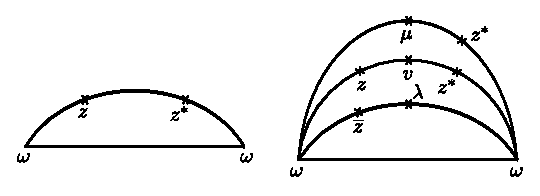
\includegraphics{fig3.eps}
\end{figure}

In\pageoriginale either case, $\epsilon>1$ and consequently
$\epsilon'<1$ so that $\epsilon-\epsilon'>0$. But
$\epsilon-\epsilon'=\gamma(\omega-\omega')$ implies that $\gamma>0$.

Now, if $z$ lies on $\omega'v\omega$, $u$ is purely imaginary with
$\arg u=\pi/2$. On setting $u=u'i$, we obtain the transformation
$u'\to {u'}^{\ast}=\epsilon^{2}u'$; $u'$ is real and
positive. Hereafter we need not distinguish between the two cases.

If we define $v$ such that $u=\epsilon^{2v}$ (writing $u$ instead of
$u'$) then $u\to u^{\ast}$ becomes $v\to v+1$. The function
$f(z,s)=y^{s}{\mathop{\sum}'}_{m,n}|m+nz|^{-2s}$, is invariant under
the modular substitution $z\to (\alpha z+\beta)(\gamma z+\delta)^{-1}$
and hence as a function of $v$, it has period $1$. It has a valid
Fourier expansion in $v$ of the form
$f(z,s)=\sum\limits^{\infty}_{k=-\infty}a_{k}e^{2\pi ikv}$. Now 
\begin{align*}
a_{k} &= \int^{1}_{0}f(z,s)e^{-2\pi ikv}dv\\
&= \frac{1}{2\log \epsilon}\int^{\epsilon^{2}}_{1}f(z,s)u^{-\pi
  ik/\log \epsilon}\frac{du}{u}.  
\end{align*}

On changing the variable from $u$ to $z$, the series $f(z,s)$ being
uniformly convergent on the corresponding segment of $\omega'v\omega$,
we may interchange integration and summation and obtain
$$
a_{k}=\frac{1}{2\log
  \epsilon}\sum_{m,n}\int^{\epsilon^{2}}_{1}\frac{y^{s}}{|m+nz|^{2s}}u^{-\pi
  ik/\log \epsilon}\frac{du}{u}.
$$
From the relation $z=\dfrac{\omega ui+\omega'}{ui+1}$ it follows that
$$
y=\frac{u(\omega-\omega')}{u^{2}+1}\text{ and }
m+nz=\frac{(m+n\omega)ui+(m+n\omega')}{ui+1} 
$$
Setting $\beta=m+n\omega$ then $\beta\in \mathfrak{b}$ since $m$ and
$n$ are both rational integers and
$\omega-\omega'=N(\mathfrak{b})\sqrt{d}$. Then our integral becomes
$$
a_{k}=\frac{1}{2\log
  \epsilon}(N(\mathfrak{b}))^{s}d^{s/2}\sum_{\mathfrak{b}|\beta\neq
  0}\int^{\epsilon^{2}}_{1}\left(\frac{u}{\beta^{2}u^{2}+{\beta'}^{2}}\right)^{s}u^{-\pi
  ik/\log\epsilon}\frac{du}{u}. 
$$
To bring the right hand-side to proper shape again, we use an idea of
Hecke. We shall now get rid of $\beta$ in the integrand by introducing
$U=u|\beta/\beta'|$.\pageoriginale The integral then reduces to
$$
\left|\frac{\beta}{\beta'}\right|^{\pi
  ik/\log\epsilon}|N(\beta)|^{-s}\int^{|(\beta\epsilon/\beta'\epsilon')|}_{|\beta/\beta'|}\frac{u^{s-(\pi
    ik/\log \epsilon)}}{(u^{2}+1)^{s}}\frac{du}{u},
$$
on writing $u$ instead of $U$. For two elements $\beta$, $\gamma$,
$\neq 0$, $(\beta)=(\gamma)$ implies that
$\gamma=\pm\beta\epsilon^{n}$, $n=0$, $\pm 1$, $\pm 2,\ldots$ with
$\epsilon>1$, being the fundamental unit in $\bQ(\sqrt{d})$. Then
$$
|\gamma|=|\beta\epsilon^{n}|,|\gamma'|=|\beta'{\epsilon'}^{n}|\text{
  and }
\left|\frac{\gamma}{\gamma'}\right|=\left|\frac{\beta\epsilon^{n}}{\beta'{\epsilon'}^{n}}\right|.
$$
We have therefore, on taking into account $\gamma=\beta\epsilon^{n}$
of $\gamma=-\beta\epsilon^{n}$,
\begin{align*}
& \sum_{\mathfrak{b}|\beta\neq
    0}\int^{|(\beta\epsilon/\beta'\epsilon')|}_{|\beta/\beta'|}
  \frac{u^{s-(\pi ik/\log\epsilon)}}{(u^{2}+1)^{s}}\frac{du}{u}\\
&= 2\sum_{\mathfrak{b}|(\beta)\neq
    0}\sum^{\infty}_{n=-\infty}\int^{|(\beta\epsilon^{n+1}/\beta'{\epsilon'}^{n+1})|}_{|(\beta\epsilon^{n}/\beta'{\epsilon'}^{n})|}\frac{u^{s-(\pi
      ik/\log\epsilon)}}{(u^{2}+1)^{s}}\frac{du}{u}. 
\end{align*}

Now since $\epsilon>1$, the intervals $(|\beta/\beta')\cdot
\epsilon^{2n}$, $|\beta/\beta'|\cdot\epsilon^{2(n+1)})$ fill out the
half-line $(0,\infty)$ exactly once, without gaps and overlaps, as $n$
tends to $-\infty$ on one side and $+\infty$ on the other side. Hence
we have
$$
2\sum^{\infty}_{n=-\infty}\int^{|(\beta\epsilon^{n+1}/\beta'{\epsilon'}^{n+1})|}_{|(\beta\epsilon^{n}/\beta'{\epsilon'}^{n})|}\frac{u^{s-(\pi
    ik/\log
    \epsilon)}}{(u^{2}+1)^{s}}\cdot\frac{du}{u}=2\int^{\infty}_{0}\frac{u^{s-(\pi
    ik/\log\epsilon)}}{(u^{2}+1)^{s}}\cdot \frac{du}{u}, 
$$
and
$$
2\int^{\infty}_{0}\frac{u^{s-(\pi
    ik/\log\epsilon)}}{(u^{2}+1)^{s}}\frac{du}{u}=\frac{\Gamma\left(\dfrac{s}{2}-\dfrac{\pi
    ik}{2\log \epsilon}\right)\Gamma\left(\dfrac{s}{2}+\dfrac{\pi
    ik}{2\log \epsilon}\right)}{\Gamma(s)}
$$
Therefore, we have
\begin{align*}
a_{k} &= \int^{1}_{0}f(z,s)e^{-2\pi ikv}dv\\
&=\frac{1}{2\log
  \epsilon}(N(\mathfrak{b}))^{s}d^{s/2}\frac{\Gamma\left(\dfrac{s}{2}-\dfrac{\pi
    ik}{2\log \epsilon}\right)\Gamma\left(\dfrac{s}{2}+\dfrac{\pi
    ik}{2\log \epsilon}\right)}{\Gamma(s)}\times\\
&\quad \times \sum_{\mathfrak{b}|(\beta)\neq
  0}\left|\frac{\beta}{\beta'}\right|^{\pi ik/\log \epsilon}|N(\beta)|^{-s},
\end{align*}\pageoriginale
since the expression under the summation $\Sigma$ does not change for
associated elements $\beta$ and $\gamma$.

Upto a product of $\Gamma$-factors, the Fourier coefficients $a_{k}$
are Dirichlet series.

For $k=0$,
\begin{align*}
a_{0}=\int^{1}_{0}f(z,s)dv &= \frac{1}{2\log \epsilon}
\frac{\Gamma^{2}\left(\dfrac{s}{2}\right)}{\Gamma(s)}d^{s/2}\sum_{\mathfrak{a}\in
  A}(N(\mathfrak{a}))^{-s}\\
&=
\frac{1}{2\log\epsilon}\frac{\Gamma^{2}\left(\dfrac{s}{2}\right)}{\Gamma(s)}d^{s/2}\zeta(s,A), 
\end{align*}
where $A$ denotes the ideal class of $\mathfrak{b}^{-1}$ in the wide
sense. If $k\neq 0$, we define for $\sigma>1$,
\begin{align*}
\zeta(s,\hat{\chi},A) &= \sum_{\mathfrak{a}\in
  A}\hat{\chi}(\mathfrak{a})(N(\mathfrak{a}))^{-s}\\
&= (\hat{\chi}(\mathfrak{b}))^{-1}\sum_{\substack{\mathfrak{a}\in
    A\\ \mathfrak{ab}=(\beta)}}\hat{\chi}((\beta))(N(\mathfrak{a}))^{-s}; 
\end{align*}
The function $\zeta(s,\hat{\chi},A)$ is called the zeta-function
of the class $A$ and associated with the Gr\"ossencharacter
$\hat{\chi}$, which is defined as follows:

The character $\hat{\chi}$ is defined on principal ideals
$(\beta)$ of $K_{0}$ as
$$
\hat{\chi}((\beta))=\left|\frac{\beta}{\beta'}\right|^{\pi
  ik/\log\epsilon}
$$
($\hat{\chi}((\beta))$ is independent of the generator $\beta$ by
definition). Then $\hat{\chi}$ is extended to all ideals
$\mathfrak{i}$ as follows: If $\mathfrak{i}^{k}=(v)$, define
$\hat{\chi}(\mathfrak{i})$ as a $h^{\text{th}}$ root of
$\hat{\chi}((v))$ so that 
$$
\hat{\chi}(\mathfrak{i}^{h})=\hat{\chi}((v))=\left|\frac{v}{v'}\right|^{\pi
  ik/\log\epsilon}
$$\pageoriginale
It is clear that $\hat{\chi}$ is multiplicative.

We have now
\begin{align*}
\hat{\chi}(\mathfrak{b})\zeta(s,\hat{\chi},A) &=
\sum_{\substack{\mathfrak{a}\in A\\ \mathfrak{ab}=(\beta)\neq
    (0)}}\hat{\chi}((\beta))(N(\mathfrak{a}))^{-s}\\
&=
(N(\mathfrak{b}))^{s}\sum_{\mathfrak{b}|(\beta)\neq(0)}\hat{\chi}((\beta))|N(\beta)|^{-s}, 
\end{align*}
so that we may rewrite the expression for $a_{k}$ as follows:
$$
a_{k}=\frac{2\log
  \epsilon}d^{s/2}\frac{\Gamma\left(\dfrac{s}{2}-\dfrac{\pi ik}{2\log
    \epsilon}\right)\Gamma\left(\dfrac{s}{2}+\dfrac{\pi ik}{2\log
    \epsilon}\right)}{\Gamma(s)}\hat{\chi}(b)\zeta(s,\hat{\chi},A).
$$

One can make some applications from the nature of the Fourier
coefficients $a_{k}$.

We know that the function $f(z,s)$ satisfies the following functional
equation, viz.
$$
\pi^{-s}\Gamma(s)f(z,s)=\pi^{-(1-s)}\Gamma(1-s)f(z,1-s).
$$

One can then show that from the analytic continuation of $f(z,s)$ it
follows that the {\em Fourier coefficients $a_{k}$ as functions of $s$
  have also analytic continuations into the whole $s$-plane and
  satisfy a functional equation similar to the above. In the
  particular} case, when $k=0$, it follows that
$$
\pi^{-s}d^{s/2}\Gamma^{2}\left(\frac{s}{2}\right)\zeta(s,A)=\pi^{-(1-s)}d^{(1-s)/2}\Gamma^{2}\left(\frac{1-s}{2}\right)\zeta(1-s,A).
$$
Hence, for the zeta-function
$\zeta_{k_{0}}(s)=\sum\limits_{A}\zeta(s,A)$, we have
$$
\pi^{-s}d^{s/2}\Gamma^{2}\left(\frac{s}{2}\right)\zeta_{K_{0}}(s)=\pi^{-(1-s)}d^{(1-s)/2}\Gamma^{2}\left(\frac{1-s}{2}\right)\zeta_{K_{0}}(1-s).
$$

This was discovered first, by Hecke, who also introduced the
zeta-functions with Gr\"ossencharacters and derived a functional
equation for the same.

We\pageoriginale shall now use Kronecker's first limit formula to
study the behaviour of $\zeta(s,A)$ at $s=1$.

From Kronecker's first limit formula, we have
$$
f(z,s)=\frac{\pi}{s-1}+2\pi(C-\log
2-\log\sqrt{y}|\eta(z)|^{2}+\cdots).
$$
It can be shown that the series on the right can be integrated term by
term with respect to $v$ (after transforming $z$ into $v$) in the
interval $(0,1)$, \ie
\begin{align*}
\int^{1}_{0}f(z,s)dv &= \frac{1}{2\log
  \epsilon}\frac{\Gamma^{2}\left(\dfrac{s}{2}\right)}{\Gamma(s)}d^{s/2}\zeta(s,A)\\
&= \frac{\pi}{s-1}+2\pi(C-\log 2)-2\pi
\int^{1}_{0}\log(\sqrt{y}|\eta(z)|^{2})dv+\cdots. 
\end{align*}

It follows therefore that the function on the left has a pole at $s=1$
with residue $\pi$ and the constant term in the expansion is provided
by the integral which cannot in general be computed. It is to be noted
here that in the case of the imaginary quadratic field, we had only
the integrand on the right side and the argument $z$ was an element of
the field, but here $z$ is a (complex) variable. One cannot get rid of
the integral even if one uses the series expansion for the integrand.

The above formula was found by Hecke and is the {\bf Kronecker limit
  formula for a real quadratic field}. One can also consider $a_{k}$
for $k\neq 0$ and obtain a similar formula.

Changing this integral to a contour integral, we shall later obtain an
analogue of Kronecker's solution of Pell's equation in terms of
elliptic functions.

We have now, for real $v$,
\begin{align*}
a_{0}=\int^{1}_{0}f(z,s)dv &= \int^{v+1}_{v}f(z,s)dv\\
&= \frac{1}{2\log
  \epsilon}\frac{\Gamma^{2}\left(\dfrac{s}{2}\right)}{\Gamma(s)}d^{s/2}\zeta(s,A). 
\end{align*}
Using\pageoriginale the Legendre formula
$$
\Gamma\left(\frac{s}{2}\right)\Gamma\left(\frac{s+1}{2}\right)=\sqrt{\pi}2^{1-s}\Gamma(s), 
$$
we obtain
$$
\frac{\Gamma(s)}{\Gamma^{2}\left(\dfrac{s}{2}\right)}=\frac{\Gamma(s)}{\Gamma^{2}\left(\dfrac{s}{2}\right)}\frac{\Gamma^{2}\left(\dfrac{s+1}{2}\right)}{\Gamma^{2}\left(\dfrac{s+1}{2}\right)}=\frac{\Gamma^{2}\left(\dfrac{s+1}{2}\right)}{\pi
  2^{2(1-s)}\Gamma(s)}.
$$
But on the other hand,
$$
\frac{\Gamma^{2}\left(\dfrac{s+1}{2}\right)}{\Gamma(s)}=1+\text{ terms
  in } (s-1)^{2},
$$
so that we have
\begin{align*}
\zeta(s,A) &= 2\log \epsilon
d^{-s/2}\frac{\Gamma(s)}{\Gamma^{2}\left(\dfrac{s}{2}\right)}\int^{v+1}_{v}f(z,s)dv
\\
&=\frac{2\log
  \epsilon}{\pi\sqrt{d}}(2^{2}d^{-\frac{1}{2}})^{(s-1)}(1+\text{ terms
  in } (s-1)^{2})\int^{v+1}_{v}f(z,s)dv. 
\end{align*}
By setting $(2^{2}d^{-\frac{1}{2}})^{(s-1)}=e^{(s-1)(2\log
  2-2\log\sqrt[4]{d})}$ and expanding it in powers of $(s-1)$, and
applying Kronecker's first limit formula for $f(z,s)$, we obtain
finally,
\begin{align*}
\zeta(s,A) &= \frac{2\log \epsilon}{\pi\sqrt{d}}(1+(s-1)(2\log
2-2\log\sqrt[4]{d})+\cdots)\times\\
&\quad \times \pi \left(\frac{1}{s-1}+2C-(2\log 2-2\log
\sqrt[4]{d})-\right.\\
&\quad
\left. -2\int^{v+1}_{v}\log(\sqrt{y}\sqrt[4]{d}|\eta(z)|^{2})dv+\cdots\right), 
\end{align*}
\ie
\begin{equation*}
\zeta(s,A)=\frac{2\log
  \epsilon}{\sqrt{d}}\left(\frac{1}{s-1}+2C-2\int^{v+1}_{v}\log
(\sqrt{y}\sqrt[4]{d}|\eta(z)|^{2})dv+\cdots\right).\tag{79}\label{79} 
\end{equation*}
From\pageoriginale this, we deduce that $\zeta(s,A)$ has a pole at
$s=1$ with residue $\dfrac{2\log \epsilon}{\sqrt{d}}$ which is
independent of the ideal class $A$. This result was first discovered
by Dirichlet.

It would be nice if one could compute the integral and express it in
terms of an analytic function, but it looks impossible. We shall only
simplify it to a certain extent by converting it into a contour
integral.

From the substitution $ui=\dfrac{z-\omega'}{\omega-z}$ follows that
$$
u=\Iim\left(\dfrac{z-\omega'}{\omega-z}\right)=\frac{y(\omega-\omega')}{(z-\omega)(\ob{z}-\omega)} 
$$
and similarly
$$
u^{-1}=\frac{y(\omega-\omega')}{(z-\omega')(\ob{z}-\omega')}.
$$
On multiplying the two, we have
\begin{equation*}
1=\frac{y^{2}}{\left\{\dfrac{(z-\omega)(z-\omega')}{\omega-\omega'}\right\}\left\{\dfrac{(\ob{z}-\omega)(\ob{z}-\omega')}{\omega-\omega'}\right\}}.\tag{80}\label{80} 
\end{equation*}
Consider now the expression
\begin{equation*}
F(z)=\frac{(z-\omega)(z-\omega')}{N(\mathfrak{b})}=az^{2}+bz+c.\tag{81}\label{81} 
\end{equation*}
We then claim that $a$, $b$, $c$ are rational with $(a,b,c)=1$ and
$b^{2}-4ac=d$. From Kronecker's generalization of Gauss's theorem on
the content of a product of polynomials with algebraic numbers as
coefficients, we have for the product
$(\xi-\omega\eta)(\xi-\omega'\eta)$,
$(1,-\omega)(1,-\omega')=(1,-(\omega+\omega'),\omega\omega')$ or in
other words, $\mathfrak{bb}'=(1,\lambda,\mu)$ where $\lambda$ and
$\mu$ are rational, \ie
$$
\left(\frac{1}{N(\mathfrak{b})},\frac{\lambda}{N(\mathfrak{b})},\frac{\mu}{N(\mathfrak{b})}\right)=1. 
$$
But, from our definition of $F(z)$, $a=\dfrac{1}{N(\mathfrak{b})}$,
$b=\dfrac{\lambda}{N(\mathfrak{b})}$, $c=\dfrac{\mu}{N(\mathfrak{b})}$
so that $(a,b,c)=1$. The discriminant of $F(z)$ is 
$$
b^{2}-4ac=\frac{(\omega+\omega')^{2}-4\omega\omega'}{N(\mathfrak{b})^{2}}=\frac{(\omega-\omega')^{2}}{N(\mathfrak{b})^{2}}=d.
$$\pageoriginale
Further $a=\dfrac{1}{N(\mathfrak{b})}>0$. We can then show that the
class of the quadratic form $F(z)$ is uniquely determined by the ideal
class $A$.

From \eqref{80} it follows that $y^{2}d=F(z)\cdot F(\ob{z})$ or
equivalently, $\sqrt{y}\sqrt[4]{d}=\sqrt[4]{F(z)\cdot F(\ob{z})}$.

Now, for the integral in \eqref{79}, we have
$$
\frac{-4\log
  \epsilon}{\sqrt{d}}\int^{v+1}_{v}\log(\sqrt{u}\sqrt[4]{d}|\eta(z)|^{2})dv=2\int^{z^{\ast}}_{z}\log(|\sqrt[4]{F(z)}\eta(z)|^{2})\dfrac{dz}{F(z)},
$$
since, by definition of $v$,
$$
dv=\frac{-\sqrt{d}}{2\log \epsilon}\cdot \frac{dz}{F(z)}
$$
and the transformation $v\to v+1$ corresponds to $z\to z^{\ast}$ on
the segment of the orthogonal circle. On the right side, $z$ may be
taken arbitrarily on the segment.

Thus, let $A$ be an ideal class, in the wide sense, of
$K_{0}=\bQ(\sqrt{d})$, $d>0$ and $\mathfrak{b}$ an ideal in $A$ with
an integral basis $[1,\omega]$, $\omega>\omega'$. Corresponding to
$\mathfrak{b}$, let $\left(\begin{smallmatrix}\alpha & \beta \\ \gamma
  & \delta\end{smallmatrix}\right)$ be defined as on $p$.\@ 85 and let
  for $z\in \mathfrak{h}$, $z^{\ast}=(\alpha z+\beta)(\gamma
  z+\delta)^{-1}$. Let, further, $\epsilon>1$ be the fundamental unit
  in $K_{0}$. Then we have

\begin{thm}[{\bf Hecke}]\label{thm8}
For the zeta-function $\zeta(s,A)$ associated with the class $A$, we
have the limit formula
$$
\lim\limits_{s\to
  1}\left(\zeta(s,A)-\frac{2\log\epsilon}{\sqrt{d}}\frac{1}{s-1}\right)=\frac{4C\log\epsilon}{\sqrt{d}}+2\int^{z^{\ast}}_{z}\log(|\sqrt[4]{F(z)}\eta(z)|^{2})\frac{dz}{F(z)}, 
$$
where the integration is over a segment $zz^{\ast}$ of the semicircle
on $\omega'\omega$ as diameter and $F(z)$ is defined by \eqref{81}.
\end{thm}

Now, the question arises whether one could transform the integral in
such\pageoriginale a way that it is independent of the choice of $z$
and also the path of integration. It is possible to do that, by the
method of Herglotz who reduced this to an integral involving simpler
functions than $\eta(z)$.

If $N(\epsilon)=1$, then the transformation $v\to v+1$ is equivalent
to $z\to z^{\ast}=\dfrac{\alpha z+\beta}{\gamma z+\delta}$ with
$\left(\begin{smallmatrix} \alpha & \beta\\ \gamma & \delta
\end{smallmatrix}\right)$, a modular matrix.

If $N(\epsilon)=-1$, on replacing $\epsilon$ by $\epsilon^{2}$,
$N(\epsilon^{2})=1$ and the transformation $v\to v+1$ goes over to the
transformation $z\to \dfrac{\alpha'z+\beta'}{\gamma'z+\delta'}$ with
$\left(\begin{smallmatrix} \alpha' & \beta'\\ \gamma' & \delta'
\end{smallmatrix}\right)$ a modular matrix. Further, because of the
periodicity of $f(z,s)$,
$$
\int^{v+2}_{v}f(z,s)dv=2\int^{v+1}_{v}f(z,s)dv
$$
so that we may assume without loss of generality that $N(\epsilon)=1$.

Now, the behaviour of $\sqrt[4]{F(z)}\cdot \eta(z)$ under a modular
substitution can be studied. We know that
$\eta(z^{\ast})=\rho\sqrt{\gamma z+\delta}\eta(z)$ where $\rho$ is a
$24$th root of unity. Further,
$$
(z^{\ast}-\omega)(z^{\ast}-\omega')=\frac{(z-\omega)(z-\omega')}{(\gamma
  z+\delta)^{2}} 
$$
if one uses the fact that $\omega=\omega^{\ast}$ and
$\gamma\omega+\delta=\epsilon$. 

From these two, it follows that
$$
\sqrt[4]{F(z^{\ast})}=\kappa\frac{\sqrt[4]{F(z)}}{\sqrt{\gamma
    z+\delta}}
$$
with $\kappa$, a $4$th root of unity. Therefore
\begin{equation*}
\sqrt[4]{F(z^{\ast})}\eta(z^{\ast})=\rho\kappa\sqrt[4]{F(z)}\eta(z).\tag{82}\label{82} 
\end{equation*}
(We emphasize here that \eqref{82} holds only for a hyperbolic
substitution and a power of the same, since we have made essential use
of the fact that $\omega$ and $\omega'$ are fixed points of the
substitution in obtaining the transformation formula for $F(z)$.)

Consider the function $\sqrt[4]{F(z)}\eta(z)$. It is an analytic
function having no zeros in the upper half plane so that on choosing a
single valued branch of\pageoriginale $\log(\sqrt[4]{F(z)}\eta(z))$,
we have a regular function in the upper $z$-half plane.

Let us denote $\log\sqrt[4]{F(z)}\eta(z)$ by $g(v)$. Then \eqref{82}
implies that $g(v+1)-g(v)=2\pi i\lambda$ (say) with $\lambda$
rational. One can then express $\lambda$ by means of the so-called
Dedekind sums. Setting $g(v)-2\pi i\lambda v=h(v)$, we have
$h(v+1)=h(v)$ possesses a Fourier development in $e^{2\pi iv}$, or in
other words, $h(v)=\sum\limits^{\infty}_{n=-\infty}c_{n}e^{2\pi inv}$,
where $c_{n}$ are constants, since $h(v)$ is an analytic function of
$v$ and $c_{0}=\int^{v+1}_{v}h(v)dv$. Here $v$ lies in a certain strip
enclosing the real axis.

Now, consider the complex integral $c_{0}=\int^{v+1}_{v}h(v)dv$. Here
$v$ is, in general, complex and the path of integration may be any
curve between $v$ and $v+1$ lying in the strip in which the Fourier
expansion is valid. We have
\begin{align*}
-\frac{\sqrt{d}}{2\log
  \epsilon}\int^{z^{\ast}}_{z}\log(|\sqrt[4]{F(z)}\eta(z)|^{2})\frac{dz}{F(z)}
&= 2\int^{v+1}_{v}\text{ Re\,}(g(v))dv\quad(v\text{ real})\\
&= 2 \text{ Re\,}\left(\int^{v+1}_{v}h(v)dv\right)\\
&= 2\text{ Re\,}(c_{0}).
\end{align*}

The computation of the integral on the left side therefore reduces to
the determination of $c_{0}$, which in turn is independent of $v$ and
the path of integration. The trick for computing the integral is to
convert it into an infinite integral by letting $z\to \infty$ and
$z^{\ast}\to \alpha/\gamma$. Expanding $g(v)$ in an infinite series,
one can express this infinite integral as a definite integral of an
elementary function. (See G.\@ Herglotz.)

We shall now obtain an analogue of Kronecker's solution of Pell's
equation in this case. Let us define
\begin{equation*}
g(A)=2\int^{z^{\ast}}_{z}\log(|\sqrt[4]{F(z)}\eta(z)|^{2})\frac{dz}{F(z)}.\tag{83}\label{83} 
\end{equation*}
Then, associated with a character $\chi$ of the ideal class group (in
the wide sense), we have
$$
L(s,\chi)=\sum_{A}\chi(A)\zeta(s,A),
$$
the\pageoriginale summation running over all wide classes $A$.

From \eqref{79}, we obtain, for $\chi\neq 1$, the expansion,
\begin{equation*}
L(s,\chi)=\sum_{A}\chi(A)g(A)+\text{ terms involving }(s-1).\tag{84}\label{84}
\end{equation*}

Before proceeding to derive the analogue of Kronecker's solution of
Pell's equation from the above, we shall examine under what
conditions, a genus character, which is a character of the narrow
class group of $\bQ(\sqrt{d})$, is also a character of the wide class
group. Let $\chi$ be a genus character, defined as follows: If
$d=d_{1}d_{2}$, then for all ideals $\mathfrak{a}$ with
$(\mathfrak{a},d_{1})=(1)$, $\chi$ is defined by
$\chi(\mathfrak{a})=\left(\dfrac{d_{1}}{N(\mathfrak{a})}\right)$. (We
may suppose without loss of generality that $d_{1}$ is odd). Now, in
general, $\chi$ is not a character of the wide class group. It will be
so, if $\chi((\alpha))=1$ for all integers $\alpha$ with
$(\alpha,d_{1})=(1)$. For elements $\alpha$ with $N(\alpha)>0$, this
is true by the definition of $\chi$.

If $N(\alpha)<0$, then
$$
\chi((\alpha))=\left(\dfrac{d_{1}}{N((\alpha))}\right)=\left(\dfrac{d_{1}}{-N(\alpha)}\right)=1 
$$
for all $\alpha$, if it is true for one such $\alpha$.

Take $\alpha=1+\sqrt{d}$ so that $N(\alpha)=1-d<0$. We need examine
only $\left(\dfrac{d_{1}}{d-1}\right)$, $d_{1}$ being odd. Then
$$
\left(\frac{d_{1}}{d-1}\right)=\left(\frac{d-1}{d_{1}}\right)=\left(\frac{-1}{d_{1}}\right)=
\begin{cases}
+1\text{ if }d_{1}>0\\
-1 \text{ if } d_{1}<0.
\end{cases}
$$

Since $d$ is positive, either both $d_{1}$, $d_{2}$ are positive or
both are negative. In the former case, $\chi$ continues to be a
character of the wide class group and in the latter case, it is no
longer a character of the wide class group.

\textsc{Case} (i).~Let us assume, that {\em both $d_{1}$ and $d_{2}$
  are positive.} Then the genus character $\chi$ as defined above, is
also a wide class character.

We have a decomposition of $L(s,\chi)$ due to Kronecker, from
\eqref{66} as follows: $L(s,\chi)=L_{d_{1}}(s)L_{d_{2}}(s)$ and on
taking the values on both sides at $s=1$,\pageoriginale we obtain
$$
L(1,\chi)=L_{d_{1}}(1)L_{d_{2}}(1).
$$

From \eqref{84}, we have now $L(1,\chi)=\sum\limits_{A}\chi(A)g(A)$,
summation running over all wide classes $A$.

Further
$$
L_{d_{1}}(1)=\frac{2\log \epsilon_{1}h_{1}}{\sqrt{d_{1}}}
$$
if $\epsilon_{1}$ denotes the fundamental unit of $\bQ(\sqrt{d_{1}})$
and $h_{1}$, the wide class number of $\bQ(\sqrt{d_{1}})$ and
similarly for $L_{d_{2}}(1)$. Thus as an analogue of Kronecker's
solution of Pell's equation as derived in \eqref{68}, we have the
following

\begin{proposition}\label{prop13}
Let $\chi$ be a genus character of $\bQ(\sqrt{d})$, $d>0$,
corresponding to the decomposition $d=d_{1}d_{2}(d_{1}>0,d_{2}>0)$ of
$d$. Let $h_{1}$, $h_{2}$ be the class numbers and $\epsilon_{1}$,
$\epsilon_{2}$ the fundamental units of $\bQ(\sqrt{d_{1}})$,
$\bQ(\sqrt{d_{2}})$ respectively. Then
\begin{equation*}
4h_{1}h_{2}\log \epsilon_{1}\log
\epsilon_{2}=\sqrt{d}\sum_{A}\chi(A)g(A),\tag{85}\label{85} 
\end{equation*}
where $A$ runs over all the ideal classes of $\bQ(\sqrt{d})$ in the
wide sense and $g(A)$ is defined by \eqref{83}.
\end{proposition}

The expression on the right side of \eqref{85} is not very simple. It
is not known whether the number on the left side is rational or
irrational. It is probable that the number on the left side is a
complicated transcendental number, so that one cannot expect a simple
value on the right side.

\textsc{Case} (ii).~Suppose $d_{1}$ and $d_{2}$ are both
negative. Then again from the decomposition formula \eqref{66}, we
have
$$
L(1,\chi)=L_{d_{1}}(1)L_{d_{2}}(1)=\frac{2\pi
  h_{1}}{w_{1}\sqrt{|d_{1}|}}\frac{2\pi h_{2}}{w_{2}\sqrt{|d_{2}|}}=\frac{4\pi^{2}h_{1}h_{2}}{w_{1}w_{2}\sqrt{d}}
$$
where $h_{1}$, $h_{2}$ denote the wide class numbers of
$\bQ(\sqrt{d_{1}})$ and $\bQ(\sqrt{d_{2}})$, and $w_{1}$, $w_{2}$ the
number of roots of unity in $\bQ(\sqrt{d_{1}})$ and
$\bQ(\sqrt{d_{2}})$ respectively. 

We\pageoriginale shall see in \S \ref{chap2:sec5} that
$$
L(1,\chi)=\frac{\pi^{2}}{\sqrt{d}}\sum_{B}\chi(B)G(B),
$$
$B$ running over all narrow classes of $\bQ(\sqrt{d})$ and $G(B)$
being numbers depending only on $B$.

We shall further prove that $G(B)$ are rational numbers which can be
realized in terms of periods of certain abelian integrals of the third
kind.

We then have, as an analogue of Kronecker's solution of Pell's
equation, the following:
$$
\frac{4h_{1}h_{2}}{w_{1}w_{2}}=\sum_{B}\chi(B)G(B).
$$

\begin{example*}
Consider the field $\bQ(\sqrt{10})$ with discriminant $d=40=5.8$;
$d_{1}=5$ and $d_{2}=8$.

The class number of $\bQ(\sqrt{10})$ is $2$. Since the fundamental
unit $\epsilon=3+\sqrt{10}$ has norm $-1$, the narrow classes are the
same as wide classes. We can now choose the two ideal class
representatives as follows
$$
(1)=\mathfrak{b}_{1}=[1,\sqrt{10}]\text{ \ and \ }
\mathfrak{b}_{2}=\left[1,\frac{1}{2}\sqrt{10}\right]\text{ \ with \ }
N(\mathfrak{b}_{2})=\frac{1}{2}. 
$$
The class numbers $h_{1}$ and $h_{2}$ of $\bQ(\sqrt{5})$ and
$\bQ(\sqrt{8})$ are both $1$ and the fundamental units are
respectively $\dfrac{1+\sqrt{5}}{2}$ and $1+\sqrt{2}$. The only
character $\chi\neq 1$ has the property that
$\chi(\mathfrak{b}_{1})=1$ and $\chi(\mathfrak{b}_{2})=-1$, so that we
have from \eqref{85}, the following:
$$
2\log\left(\frac{1+\sqrt{5}}{2}\right)\cdot\log
(1+\sqrt{2})=\sqrt{10}(g(E)-g(A)). 
$$
\end{example*}

We shall make a remark for more general applications. Consider the
absolute class field of $\bQ(\sqrt{d})$ with $d>0$. For computing the
class number of this field, one can proceed in the same way, as in the
case of an imaginary quadratic field. For the same, one requires the
computation of $L(1,\chi)$ for arbitrary narrow class characters. This
will be done in \S\ \ref{chap2:sec5}, for a special type of
characters.

\section{Ray class fields over $\bQ(\sqrt{d})$,
  $d<0$}\label{chap2:sec4} 
\pageoriginale
%%%% 4

Let $K$ be an algebraic number field of degree $n$ over $\bQ$, the
field of rational numbers. Let $r_{1}$ and $2r_{2}$ be the number of
real and complex conjugates of $K$ respectively, so that
$r_{1}+2r_{2}=n$. Let $K^{(1)},\ldots,K^{(r_{1})}$ be the real
conjugates of $K$ and $K^{(r_{1}+1)},\ldots,K^{(n)}$ be the complex
conjugates of $K$. Let, for $\alpha\in K$, $\alpha^{(i)}\in K^{(i)}$,
$i=1,2,\ldots,n$, denote the conjugates of $\alpha$. Further let
$\mathfrak{f}$ be a given integral ideal in $K$. Two numbers
$\gamma_{1}=\dfrac{\alpha_{1}}{\beta_{1}}$,
$\gamma_{2}=\dfrac{\alpha_{2}}{\beta_{2}}$ with $\alpha_{1}$,
$\beta_{1}$, $\alpha_{2}$, $\beta_{2}$ integral in $K$ and with
$\beta_{1}\beta_{2}$ coprime to $\mathfrak{f}$ are
{\em(multiplicatively) congruent modulo $\mathfrak{f}$} (in symbols,
$\gamma_{1}\equiv \gamma_{2}(\rm{mod} \;^{\ast}\mathfrak{f})$ if
$\alpha_{1}\beta_{2}\equiv \alpha_{2}\beta_{1}(\rm{mod} \;
\mathfrak{f})$). If $\gamma_{1}$, $\gamma_{2}$ are integers in $K$,
this is the usual congruence modulo $\mathfrak{f}$.

Let us consider non-zero fractional ideals $\mathfrak{a}$ of the form
$\mathfrak{a}=\dfrac{\mathfrak{b}}{\mathfrak{c}}$ where $\mathfrak{b}$
and $\mathfrak{c}$ are integral ideals in $K$ coprime to
$\mathfrak{f}$. These fractional ideals $\mathfrak{a}$ form, under the
usual multiplication of ideals, an abelian group which we shall denote
by $\mathfrak{G}_{\mathfrak{f}}$. Let $\mathfrak{G}_{\mathfrak{f}}$ be
the subgroup of $\mathfrak{G}_{\mathfrak{f}}$ consisting of all
principal ideals $(\alpha)$ for which $\alpha \succ 0$ (\ie
$\alpha^{(i)}>0$, for $i=1,2,\ldots,r_{1}$) and $\alpha\equiv
1(\rm{mod} \;^{\ast}\mathfrak{f})$. It is clear that if
$(\gamma)\in\mathfrak{G}_{\mathfrak{f}}$ and $\gamma\equiv
1(\rm{mod} \;^{\ast}\mathfrak{f})$, then $\gamma$ might be written as
$\alpha/\beta$ where $\alpha$ and $\beta$ are integers in $K$
satisfying the conditions, $\alpha \succ 0$, $\beta \succ 0$, $\alpha\equiv
1(\rm{mod} \;\mathfrak{f})$ and $\beta\equiv 1(\rm{mod} \;\mathfrak{f})$. 

The quotient group
$\mathfrak{G}_{\mathfrak{f}}/\mathfrak{G}_{\mathfrak{f}}$ is a finite
abelian group called the {\em ray class group modulo} $\mathfrak{f}$;
its elements are called {\em ray classes modulo} $\mathfrak{f}$. Two
ideals $\mathfrak{a}$ and $\mathfrak{b}$ in
$\mathfrak{G}_{\mathfrak{f}}$ are {\em equivalent modulo}
$\mathfrak{f}(\mathfrak{a}\sim \mathfrak{b}\rm{mod} \;\mathfrak{f})$ if they
lie in the same ray class modulo $\mathfrak{f}$, \ie
$\mathfrak{a}=(\gamma)\mathfrak{b}$ with
$(\gamma)\in\mathfrak{G}_{\mathfrak{f}}$.

If $r_{1}=0$ and $\mathfrak{f}=(1)$, equivalence modulo $\mathfrak{f}$
is the usual equivalence in the wide sense and the ray class group
modulo $\mathfrak{f}$ is the class group of $K$ in the wide sense. If
$r_{1}=2$, $r_{2}=0$ (\ie $K$ is a real quadratic field) and
$\mathfrak{f}=(1)$, then the equivalence modulo $\mathfrak{f}$ is the
equivalence in the narrow sense and the ray class group is the class
group of $K$ in the narrow sense. Let $\chi$ be a character of the
group of ray classes modulo $\mathfrak{f}$. Then associated with
$\chi$, we define for $\sigma>1$, the $L$-series
$$
L(s,\chi)=\sum_{\mathfrak{a}\neq
  0}\chi(\mathfrak{a})(N(\mathfrak{a}))^{-s}
$$
where $N(\mathfrak{a})$ is the norm of $\mathfrak{a}$ in $K$ and the
summation is extended over all integral ideals $\mathfrak{a}$ coprime
to $\mathfrak{f}$. It is clear that $L(s,\chi)$ is a regular
function\pageoriginale of $s$ for $\sigma>1$. Moreover, due to the
multiplicative character of $\chi$, we have for $\sigma>1$, an
Euler-product decomposition for $L(s,\chi)$, namely
$$
L(s,\chi)=\prod_{\mathfrak{p}|\mathfrak{f}}(1-\chi(\mathfrak{p})(N(\mathfrak{p}))^{-s})^{-1}
$$
where the infinite product is extended over all prime ideals
$\mathfrak{p}$ coprime to $\mathfrak{f}$.

Hecke has shown that $L(s,\chi)$ can be continued analytically as a
meromorphic function of $s$ in the whole $s$-plane and that when
$\chi$ is a ``proper'' character, there is a functional equation
relating $L(s,\chi)$ with $L(1-s,\ob{\chi})$, where $\ob{\chi}$ is the
conjugate character. If $\chi\neq 1$ (the principal character), then
$L(s,\chi)$ is an entire function of $s$. If $\chi=1$ and
$\mathfrak{f}=(1)$, then $L(s,\chi)$ is the Dedekind zeta function of
$K$.

We are interested in determining the value at $s=1$ of $L(s,\chi)$, in
the case when $K$ is a real or imaginary quadratic number field and
$\chi$ is not the principal character. For this purpose, we need to
apply Kronecker's second limit formula. Later, we shall use this for
the determination of the class number of the ``ray class field'' of
$K$, corresponding to the ideal $\mathfrak{f}$.

First we shall investigate the structure of a ray class character
$\chi$. Let $\alpha$ and $\beta(\neq 0)$ be integers coprime to
$\mathfrak{f}$ such that $\alpha=\beta(\rm{mod} \;\mathfrak{f})$. Then
$\gamma=\dfrac{\alpha^{2}}{\beta^{2}}$ satisfies
$\gamma=1(\rm{mod} \;^{\ast}\mathfrak{f})$ and $\gamma \succ 0$ so that
$\chi((\gamma))=1$ \ie $\chi((\alpha^{2}))=\chi((\beta^{2}))$. In
other words,
$$
\chi((\alpha))=\pm \chi((\beta))\quad\text{or}\quad
\chi((\alpha/\beta))=\pm 1.
$$

Let $\mathfrak{L}$ be the multiplicative group of $\lambda\neq 0$ in
$K$. Corresponding to a ray class character $\chi$ modulo
$\mathfrak{f}$, we define a character $v$ of $\mathfrak{L}$ as
follows. For $\lambda\in\mathfrak{L}$, we find an integer $\alpha\in
K$ such that $\alpha\equiv 1(\rm{mod} \; \mathfrak{f})$ and $\alpha\lambda \succ 0$
and define $v(\lambda)=\chi((\alpha))$. It is first clear that
$v(\lambda)$ is well-defined; for, if $v(\lambda)=\chi((\beta))$ for
another integer $\beta\in K$ satisfying the same conditions, then we
see at once that $\dfrac{\alpha}{\beta}\equiv
1(\rm{mod} \;^{\ast}\mathfrak{f})$ and $\dfrac{\alpha}{\beta} \succ 0$ and so
$\chi((\alpha))=\chi((\beta))$. It is easily verified that
$v(\lambda\mu)=v(\lambda)v(\mu)$. Moreover, $v(\lambda)=\pm 1$; for,
$\lambda^{2} \succ 0$ and by definition,
$v(\lambda^{2})=\chi((\alpha))$\pageoriginale for $\alpha$ satisfying
$\alpha\equiv 1(\rm{mod} \;\mathfrak{f})$ and $\alpha \succ 0$ so that
$(v(\lambda))^{2}=v(\lambda^{2})=\chi((\alpha))=+1$. We shall call
$v(\lambda)$, a {\bf character of signature.}

Consider the subgroup $\mathfrak{B}$ of $\mathfrak{L}$ consisting of
$\lambda \succ 0$. Clearly $v(\lambda)=1$ for all $\lambda\in
\mathfrak{B}$. Thus $v(\lambda)$ may be regarded as a character of the
quotient group $\mathfrak{L}/\mathfrak{B}$. Now
$\mathfrak{L}/\mathfrak{B}$ is an abelian group of order $2^{r_{1}}$
exactly, since one can find $\lambda\in\mathfrak{L}$ for which the
real conjugates $\lambda^{(i)}$, $i=1,2,\ldots,r_{1}$, have
arbitrarily prescribed signs. Also, there are $2^{r_{1}}$ distinct
characters $u$ of $\mathfrak{L}/\mathfrak{B}$ defined by
$$
u(\lambda)=\prod^{r_{1}}_{i=1}\left(\frac{\lambda^{(i)}}{|\lambda^{(i)}|}\right)^{g_{i}},\quad
g_{i}=0\text{ \ or \ } 1,\lambda\in \mathfrak{L}.
$$
There can indeed be no more that $2^{r_{1}}$ characters of
$\mathfrak{L}/\mathfrak{B}$ and hence $v(\lambda)$ coincides with one
of these characters $u$, of $\mathfrak{L}/\mathfrak{B}$. We do not
however assert that every character $u$ of $\mathfrak{L}/\mathfrak{B}$
is realizable from a ray class character modulo $\mathfrak{f}$, in the
manner described above.

Let now $\gamma\in K$ such that $\gamma\equiv
1(\rm{mod} \;^{\ast}\mathfrak{f})$ and
$(\gamma)\in\mathfrak{G}_{\mathfrak{f}}$. By definition,
$v(\gamma)=\chi((\delta))$ for an integer $\delta$ such that
$\delta\equiv 1(\rm{mod} \; \mathfrak{f})$ and $\delta\gamma \succ 0$. But
$\chi((\delta))=\chi((\gamma))$ and hence
$v(\gamma)=\chi((\gamma))$. Let $\alpha$ and $\beta(\neq 0)$ be two
integers coprime to $\mathfrak{f}$ such that
$\alpha=\beta(\rm{mod} \;\mathfrak{f})$. Then $\gamma=\alpha/\beta\equiv
1(\rm{mod} \;^{\ast}\mathfrak{f})$ and
$$
\frac{\chi((\alpha))}{\chi((\beta))}=\chi((\gamma))=v(\gamma)=\frac{v(\alpha)}{v(\beta)}. 
$$
Thus for integral $\alpha(\neq 0)$ coprime to $\mathfrak{f}$, the
ratio $\chi((\alpha))/v(\alpha)$ depends only on the residue class of
$\alpha$ modulo $\mathfrak{f}$ and is in fact, a character of the
group $G(\mathfrak{f})$ of prime residue classes modulo
$\mathfrak{f}$. We may denote it by $\chi(\alpha)$. Thus

\begin{proposition}\label{prop14}
Any character $\chi((\alpha))$ of the ray class group modulo
$\mathfrak{f}$ may be written in the form
$$
\chi((\alpha))=v(\alpha)\chi(\alpha)
$$
where $v(\alpha)$ is a character of signature and $\chi(\alpha)$ is a
character of the group $G(\mathfrak{f})$.
\end{proposition}

Before proceeding further, we give a simple illustration of the
above. Let us take $K$ to be $\bQ$, the field of rational numbers and
$\mathfrak{f}$ to be the principal\pageoriginale ideal $(|d|)$ in the
ring of rational integers, $d$ being the discriminant of a quadratic
field over $\bQ$. For an integer $m$ coprime to $d$, we define 
$$
\chi((m))=
\begin{cases}
\left(\dfrac{d}{|m|}\right)\dfrac{m}{|m|} & \text{for } d>0\\
\left(\dfrac{d}{|m|}\right) & \text{for } d<0
\end{cases}
$$
where $\left(\dfrac{d}{|m|}\right)$ is the Legendre-Jacobi-Kronecker
symbol. The group $\mathfrak{G}_{\text{f}}$ now consists of fractional
ideals $(m/n)$ where $m$ and $n$ are rational integers coprime to
$d$. We extend $\chi$ to the ideals $(m/n)$ in
$\mathfrak{G}_{\mathfrak{f}}$ by setting
$\chi((m/n))=\chi((m))/\chi((n))$. Now it is known that if $m\equiv
n(\rm{mod} \; d)$ and $mn$ is coprime to $d$, then
$$
\left(\frac{d}{|m|}\right)=\left(\frac{d}{|n|}\right)\text{ \ if \ }
d>0
$$
and
$$
\left(\frac{d}{|m|}\right)\frac{m}{|m|}=\left(\frac{d}{|n|}\right)\frac{n}{|n|}\text{
  \ if \ } d<0
$$
Thus 
$$
\chi(m)=\left(\frac{d}{|m|}\right)\quad\text{for}\quad d>0
$$
and
$$
\chi(m)=\left(\frac{d}{|m|}\right)\frac{m}{|m|}\quad\text{for}\quad
d<0
$$
are characters of $G(|d|)$. Moreover $v(m)=\dfrac{m}{|m|}$ is clearly
a character of signature. It is easily verified that $\chi((m/n))$ is
a ray class character modulo $(|d|)$ and that $\chi((m))=v(m)\chi(m)$.

Now
$L(s,\chi)=\sum\limits_{A}\sum_{\mathfrak{a}}(\mathfrak{a})(N(\mathfrak{a}))^{-s}$,
where $A$ runs over all the ideal classes in the wide sense and
$\mathfrak{a}$ over all the non-zero integral ideals in $A$, which are
coprime to $\mathfrak{f}$. In the class $A^{-1}$, we can choose an
integral ideal $\mathfrak{b}_{A}$ coprime to $\mathfrak{f}$ and
$\mathfrak{ab}_{A}=(\beta)$ where $\beta$ is an integer divisible by
$\mathfrak{b}_{A}$ and coprime\pageoriginale to
$\mathfrak{f}$. Conversely, and principal ideal $(\beta)$ divisible by
$\mathfrak{b}_{A}$ and coprime to $\mathfrak{f}$ is of the form
$\mathfrak{ab}_{A}$, where $\mathfrak{a}$ is an integral ideal in $A$
coprime to $\mathfrak{f}$. Moreover,
$\chi(\mathfrak{b}_{A})\chi(\mathfrak{a})=\chi((\beta))$ and
$N(\mathfrak{b}_{A})\cdot N(\mathfrak{a})=|N(\beta)|$, where
$N(\beta)$ is the norm of $\beta$. Thus
$$
L(s,\chi)=\sum_{A}\ob{\chi}(\mathfrak{b}_{A})(N(\mathfrak{b}_{A}))^{s}\sum_{\mathfrak{b}_{A}|(\beta)}\chi((\beta))|N(\beta)|^{-s}
$$
where the inner summation is over all principal ideals $(\beta)$
divisible by $\mathfrak{b}_{A}$ and coprime to $\mathfrak{f}$. Since
$A^{-1}$ runs over all classes in the wide sense when $A$ does so, we
may assume that $\mathfrak{b}_{A}$ is an integral ideal in $A$ coprime
to $\mathfrak{f}$. Moreover, in view of Proposition \ref{prop14}, we
have for $\sigma>1$,
\begin{equation*}
L(s,\chi)=\sum_{A}\ob{\chi}(\mathfrak{b}_{A})(N(\mathfrak{b}_{A}))^{s}\sum_{\mathfrak{b}_{A}|(\beta)}v(\beta)\chi(\beta)|N(\beta)|^{-s}\tag{86}\label{86} 
\end{equation*}
where now $A$ runs over all the ideal classes of $K$ in the wide
sense, $\mathfrak{b}_{A}$ is a fixed integral ideal in $A$ coprime to
$\mathfrak{f}$ and the inner sum is over all principal ideals
$(\beta)$ divisible by $\mathfrak{b}_{A}$ and coprime to
$\mathfrak{f}$. We may extend $\chi(\beta)$ to all residue classes
modulo $\mathfrak{f}$ by setting $\chi(\alpha)=0$ for $\alpha$ not
coprime to $\mathfrak{f}$. Thus we may regard the inner sum in
\eqref{86} as extended over all principal ideals $(\beta)$ divisible
by $\mathfrak{b}_{A}$. In order to render the series in \eqref{86}
suitable for the application of Kronecker's limit formula, we have to
replace $\chi(\beta)$ by an exponential of the form $e^{2\pi
  i(mu+nv)}$ occurring in the limit formula. We shall, in the sequel,
express $\chi(\beta)$ as an exponential sum by using an idea due to
Lagrange, which is as follows.

Let $x_{1},\ldots,x_{n}$ be $n$ distinct roots of a polynomial $f(x)$
of degree $n$, with coefficients in a field $K_{0}$ containing all the
$n^{\text{th}}$ roots of unity. Let, further, the field
$M=K_{0}(x_{1},\ldots,x_{n})$ be an abelian extension of $K_{0}$, with
galois group $H$. Let us assume moreover that if
$\sigma_{1},\ldots,\sigma_{n}\in H$, then
$x_{i}=x^{\sigma_{i}}_{1}i=1,2,\ldots,n$. Now, if $\chi$ is a
character of $H$, then let us define
$y_{\chi}=\sum\limits^{n}_{i=1}\chi(\sigma_{i})x_{i}$. It is clear
that $y_{\chi}\in M$ and 
$$
y^{\sigma_{j}}_{\chi}=\sum^{n}_{i=1}\chi(\sigma_{i})x^{\sigma_{i}\sigma_{j}}_{1}=\ob{\chi}(\sigma_{j})\sum^{n}_{i=1}\chi(\sigma_{i}\sigma_{j})x^{\sigma_{i}\sigma_{j}}_{1}=\ob{\chi}(\sigma_{j})y_{\chi}. 
$$
Hence $y^{n}_{\chi}\in K_{0}$. Now, if $\ob{\chi}$ denotes the
conjugate character of $\chi$ and $\sigma\in H$, then 
$$
y_{\ob{\chi}}=\sum^{n}_{i=1}\ob{\chi}(\sigma_{i}\sigma)x^{\sigma_{i}\sigma}_{1}=\ob{\chi}(\sigma)\sum^{n}_{i=1}\ob{\chi}(\sigma_{i})x^{\sigma}_{i}.
$$\pageoriginale
If $y_{\ob{\chi}}\neq 0$, then
$\chi(\sigma)=y^{-1}_{\ob{\chi}}\sum\limits^{n}_{i=1}\ob{\chi}(\sigma_{i})x^{\sigma}_{i}$. We
shall use a similar method to express $\chi(\beta)$ as an exponential
sum whose terms involve $\beta$ in the exponent.

First we need the following facts concerning the {\em different} of an
algebraic number field $M$ of finite degree over $\bQ$. Let for
$\alpha\in M$, $S(\alpha)$ denote the {\em trace} of $\alpha$. Let
$\mathfrak{a}$ be an ideal (not necessarily integral) in $M$ and let
$\mathfrak{a}^{\ast}$ be the ``complementary'' ideal to
$\mathfrak{a}$, namely the set of $\lambda\in M$, for which
$S(\lambda\alpha)$ is a rational integer for all
$\alpha\in\mathfrak{a}$. It is known that $\mathfrak{aa}^{\ast}$ is
independent of $\mathfrak{a}$ and in fact
$\mathfrak{aa}^{\ast}=(1)^{\ast}=\vartheta^{-1}$, where $\vartheta$ is
the {\em different} of $M$. Further clearly
$(\mathfrak{a}^{\ast})^{\ast}=\mathfrak{a}$ and $N(\vartheta)=|d|$,
where $d$ is the {\em discriminant} of $M$. These facts can be
verified in a simple way if $M$ is a quadratic field over $\bQ$, with
discriminant $d$. Let $[\alpha_{1},\alpha_{2}]$ be an integral basis
of $\mathfrak{a}$. The ideal $\mathfrak{a}^{\ast}$ is the set of
$\lambda\in M$ for which $S(\lambda\alpha_{1})$ and
$S(\lambda\alpha_{2})$ are both rational integers. If $\alpha'_{1}$,
$\alpha'_{2}$ denote the conjugates of $\alpha_{1}$ and $\alpha_{2}$
respectively, then it is easily verified that
$\left[\dfrac{\alpha'_{2}}{\alpha_{1}\alpha'_{2}-\alpha_{2}\alpha'_{1}},\dfrac{-\alpha'_{1}}{\alpha_{1}\alpha'_{2}-\alpha_{2}\alpha'_{1}}\right]$
is an integral basis of $\mathfrak{a}^{\ast}$. Now
$\alpha_{1}\alpha'_{2}-\alpha_{2}\alpha'_{1}=\pm
N(\mathfrak{a})\sqrt{d}$ and this means that
$\mathfrak{a}^{\ast}=(1/N(\mathfrak{a})\sqrt{d})\mathfrak{a}'$. Since
$(N(\mathfrak{a}))=\mathfrak{aa}'$, we see that
$\mathfrak{a}^{\ast}=\mathfrak{a}^{-1}(1/\sqrt{d})$ \ie
$\mathfrak{aa}^{\ast}=(1/\sqrt{d})=\vartheta^{-1}$. Moreover
$N(\vartheta)=|d|$.

Let us consider now the ideal
$\mathfrak{a}=\mathfrak{f}^{-1}\vartheta^{-1}$ in $K$; clearly
$\mathfrak{a}^{\ast}=\mathfrak{f}$. Let us choose in the class of
$\mathfrak{f}\vartheta$, an integral ideal $\mathfrak{q}$ coprime to
$\mathfrak{f}$. Then
$\mathfrak{q}\mathfrak{f}^{-1}\vartheta^{-1}=(\gamma)$ for $\gamma\in
K$ \ie $(\gamma)\vartheta=\mathfrak{q}\mathfrak{f}^{-1}$ has exact
denominator $\mathfrak{f}$. If $K$ were a quadratic field and
$\mathfrak{f}$, a principal ideal, then $\mathfrak{f}\vartheta$ is
principal and we may take $\mathfrak{q}=(1)$. We {\em shall consider
  $\gamma$ fixed this way once for all, in the sequel.} Let us observe
that if $\lambda\in\mathfrak{f}$, $S(\lambda\gamma)$ is a rational
integer.

With a view to express $\chi(\beta)$ as an exponential sum, we now
define the sum
\begin{equation*}
T=\sum_{\lambda\rm{mod} \;\mathfrak{f}}\ob{\chi}(\lambda)e^{2\pi
  iS(\lambda\gamma)}\tag{87}\label{87} 
\end{equation*}
where $\lambda$ runs over a full system of representatives of residue
classes modulo $\mathfrak{f}$; for $\mathfrak{f}=(1)$, clearly
$T=1$. We see that $T$ is defined independently\pageoriginale of the
choice of representatives $\lambda$, for, if $\mu$ runs over another
system of representatives modulo $\mathfrak{f}$, then $\lambda\equiv
\mu(\rm{mod} \; \mathfrak{f})$ in some order and in this case,
$\ob{\chi}(\lambda)=\ob{\chi}(\mu)$ and $e^{2\pi
  iS(\lambda\gamma)}=e^{2\pi iS(\mu\gamma)}$ since
  $S((\lambda-\mu)\gamma)$ is a rational integer. Moreover, in this
  sum, $\lambda$ may be supposed to run only over representatives of
  elements of $G(\mathfrak{f})$, since $\ob{\chi}(\alpha)=0$, for
  $\alpha$ not coprime to $\mathfrak{f}$. The sums of this type were
  first investigated by Hecke; similar sums for the case of the
  rational number field have been studied by Gauss, Dirichlet and for
  complex characters $\chi$, by Hasse.

Let $\alpha$ be an integer in $K$ coprime to $\mathfrak{f}$. Then
$\alpha\lambda$ runs over a complete set of prime residue classes
modulo $\mathfrak{f}$ when $\lambda$ $\lambda$ does so. Thus
\begin{align*}
T &= \sum_{\lambda\rm{mod} \; \mathfrak{f}}\ob{\chi}(\alpha\lambda)e^{2\pi
  iS(\alpha\lambda\gamma)}\\
&= \ob{\chi}(\alpha)\sum_{\lambda\rm{mod} \;
  \mathfrak{f}}\ob{\chi}(\lambda)e^{2\pi iS(\alpha\lambda\gamma)},
\end{align*}
\ie
\begin{equation*}
T\chi(\alpha)=\sum_{\lambda\rm{mod} \;\mathfrak{f}}\ob{\chi}(\lambda)e^{2\pi
  iS(\alpha\lambda\gamma)}.\tag{88}\label{88} 
\end{equation*}
We shall presently see that \eqref{88} is true even for $\alpha$ not
coprime to $\mathfrak{f}$ and that $T\neq 0$, when $\chi$ is a
so-called {\em proper} character of $G(\mathfrak{f})$.

Let $\mathfrak{g}$ be a proper divisor of $\mathfrak{f}$ and $\psi$, a
character of $G(\mathfrak{g})$. We may extend $\psi$ into a character
$\chi$ of $G(\mathfrak{f})$ by setting $\chi(\lambda)=\psi(\lambda)$
for $\lambda$ coprime to $\mathfrak{f}$ and $\chi(\lambda)=0$,
otherwise. We say that a character $\chi$ of $G(\mathfrak{f})$ is {\em
  proper}, if it is not derivable in this way from a character of
$G(\mathfrak{g})$ for a proper divisor $\mathfrak{g}$ of
$\mathfrak{f}$.

A ray class character $\chi$ modulo $\mathfrak{f}$ is said to be {\em
  proper} if the associated character $\chi$ of $G(\mathfrak{f})$ is
proper; $\chi$ is then said to have $\mathfrak{f}$ as {\em conductor}.

Let $\chi$ be a ray class character modulo $\mathfrak{f}$ and let
$\mathfrak{g}$ be a proper divisor of $\mathfrak{f}$. Moreover let for
integers $\alpha$, $\beta$ coprime to $\mathfrak{f}$ such that
$\alpha\equiv \beta(\rm{mod} \;\mathfrak{g})$ and $\alpha\beta \succ 0$,
$\chi(\alpha)=\chi(\beta)$. We can associate with $\chi$, a ray class
character $\chi_{0}$ modulo $\mathfrak{g}$ as follows. If
$\mathfrak{p}$ is a prime ideal coprime to $\mathfrak{f}$, define
$\chi_{0}(\mathfrak{p})=\chi(\mathfrak{p})$. If $\mathfrak{p}$ is a
prime ideal coprime to $\mathfrak{g}$ but not to $\mathfrak{f}$, we
can find a number $\alpha$ such that $\alpha\equiv
1(\rm{mod} \;^{\ast}\mathfrak{g})$, $\alpha \succ 0$ and $(\alpha)\mathfrak{p}$ is
coprime to $\mathfrak{f}$. We then set
$\chi_{0}(\mathfrak{p})=\chi((\alpha)\mathfrak{p})$. We see that
$\chi_{0}$ is well-defined for all prime\pageoriginale ideals coprime
to $\mathfrak{g}$ and we extend $\chi_{0}$ multiplicatively to all
ideals in the ray classes modulo $\mathfrak{g}$. Clearly, $\chi_{0}$
is a ray class character modulo $\mathfrak{G}$ and for integral
$\alpha$ coprime to $\mathfrak{g}$,
$\chi_{0}((\alpha))=\chi_{0}(\alpha)v(\alpha)$, where
$\chi_{0}(\alpha)$ is the associated character of $G(\mathfrak{g})$
and $v(\alpha)$ is the same signature character as the one associated
with $\chi$. We now say the ray class character $\chi$ modulo
$\mathfrak{f}$ having the property described above with respect to
$\mathfrak{g}$, has $\mathfrak{g}$ as {\em conductor}, if the
associated $\chi_{0}$ has $\mathfrak{g}$ as conductor. Let {\em from
  now on}, $\chi$ be a {\em proper} ray class character modulo
$\mathfrak{f}$. Since $\chi(\alpha)=0$ for $\alpha$ not coprime to
$\mathfrak{f}$, all we need to prove \eqref{88} for proper $\chi$ and
for $\alpha$ not coprime to $\mathfrak{f}$ is to show that the right
hand side of \eqref{88} is zero. Let $\mathfrak{b}$ be the greatest
common divisor of $(\alpha)$ and $\mathfrak{f}$ and let
$\mathfrak{g}=\mathfrak{f}\mathfrak{b}^{-1}$. Since $\chi$ is proper,
it is not derivable from any character of $G(\mathfrak{g})$. In other
words, there exist integers $\lambda$ and $\mu$ coprime to
$\mathfrak{f}$ such that $\lambda\equiv \mu(\rm{mod} \; \mathfrak{g})$ and
$\chi(\lambda)\neq \chi(\mu)$. Otherwise, if for all integers
$\lambda$ and $\mu$ coprime to $\mathfrak{f}$ and for which
$\lambda\equiv \mu(\rm{mod} \;\mathfrak{g})$ it is true that
$\chi(\lambda)=\chi(\mu)$, then we can define a character $\chi_{0}$
of $G(\mathfrak{g})$ such that for $\lambda$ coprime to
$\mathfrak{f}$, $\chi(\lambda)=\chi_{0}(\lambda)$ which is a
contradiction. Thus we can find integers $\mu$ and $\nu$ coprime to
$\mathfrak{f}$ such that $\mu\equiv v(\rm{mod} \;\mathfrak{g})$ and
$\chi(\mu)\neq \chi(v)$. Now clearly
\begin{equation*}
\sum_{\lambda\rm{mod} \;\mathfrak{f}}\ob{\chi}(\lambda)e^{2\pi
  iS(\alpha\lambda\gamma)}=
\begin{cases}
\ob{\chi}(\mu)\sum\limits_{\lambda\rm{mod} \;\mathfrak{f}}\ob{\chi}(\lambda)e^{2\pi
  iS(\alpha\lambda\gamma\mu)}\\
\ob{\chi}(v)\sum\limits_{\lambda\rm{mod} \;\mathfrak{f}}\ob{\chi}(\lambda)e^{2\pi
  iS(\alpha\lambda\gamma \nu)}.
\end{cases}\tag{89}\label{89}
\end{equation*}
Further since $\alpha\mu\equiv \alpha\nu(\rm{mod} \;\mathfrak{f})$,
$S(\alpha\lambda\gamma(\mu-\nu))$ is a rational integer and hence
$$
\sum_{\lambda\rm{mod} \;\mathfrak{f}}\ob{\chi}(\lambda)e^{2\pi
  iS(\alpha\lambda\gamma\mu)}=\sum_{\lambda\rm{mod} \;\mathfrak{f}}\ob{\chi}(\lambda)e^{2\pi
  iS(\alpha\lambda\gamma\nu)}. 
$$
But since $\ob{\chi}(\mu)\neq \ob{\chi}(\nu)$, we see from \eqref{89},
that
$$
\sum_{\lambda\rm{mod} \;\mathfrak{f}}\ob{\chi}(\lambda)e^{2\pi
  iS(\alpha\lambda\gamma)}=0.
$$
Hence \eqref{88} is true for {\em all integral} $\alpha$.

We now proceed to prove the $T\neq 0$. In fact, using \eqref{89}, we
have
\begin{align*}
T\ob{T} & =T\sum_{\alpha\rm{mod} \;\mathfrak{f}}\chi(\alpha)e^{-2\pi
  iS(\alpha\gamma)}\\
&=
\sum_{\lambda\rm{mod} \;\mathfrak{f}}\ob{\chi}(\lambda)\sum_{\alpha\rm{mod} \;\mathfrak{f}}e^{2\pi
  iS(\alpha(\lambda-1)\gamma)}\tag{90}\label{90} 
\end{align*}\pageoriginale
Now if $\alpha$ runs over a complete system of representatives of
residue classes modulo $\mathfrak{f}$, so does $\alpha+\nu$ for every
integer $\nu$ and hence
$$
\sum_{\alpha\rm{mod} \;\mathfrak{f}}e^{2\pi iS(\mu\alpha\gamma)}=e^{2\pi
  iS(\mu\gamma\nu)}\sum_{\alpha\rm{mod} \;\mathfrak{f}}e^{2\pi
  iS(\mu\alpha\gamma)} 
$$
Thus, if there exists at least one integer $\nu$ such that
$S(\mu\gamma\nu)$ is not a rational integer,
$\sum\limits_{\alpha\rm{mod} \;\mathfrak{f}}e^{2\pi
  iS(\mu\alpha\gamma)}=0$. Now $S(\mu\gamma\nu)$ is a rational integer
for all integers $\nu$ if and only if $\mu\gamma\in\vartheta^{-1}$ \ie
if and only if $(\mu)\mathfrak{qf}^{-1}$ is integral \ie
$\mu\in\mathfrak{f}$. Thus
$$
\sum_{\alpha\rm{mod} \;\mathfrak{f}}e^{2\pi iS(\mu\alpha\gamma)}=
\begin{cases}
0, & \text{if } \mu\not\in \mathfrak{f},\\
N(\mathfrak{f}), & \text{if } \mu\in \mathfrak{f}. 
\end{cases}
$$
From this and from \eqref{90}, we have then $|T|^{2}=N(\mathfrak{f})$,
\ie $|T|=\sqrt{N(\mathfrak{f})}$. The determination of the exact value
of $T/|T|$ is of the same order of difficulty as the corresponding
problem for ``generalized Gauss sums'' considered by Hasse. We have,
finally, for proper $\chi$ modulo $\mathfrak{f}$, as a consequence of
\eqref{88}, 
\begin{equation*}
\chi(\beta)=T^{-1}\sum_{\lambda\rm{mod} \; \mathfrak{f}}\chi(\lambda)e^{2\pi
  iS(\lambda\beta\gamma)}\tag{91}\label{91} 
\end{equation*}
Let us notice that $\beta$ appears in the exponent in the sum on the
right-hand side of \eqref{91}.

We now insert the value of $\chi(\beta)$ as given by \eqref{91} in the
series on the right hand side of \eqref{86}. In view of the absolute
convergence of the series for $\sigma>1$ and in view of the fact that
the sum in \eqref{93} is a finite sum, we are allowed to rearrange the
terms as we like. We then obtain for $\sigma>1$ and for a ray class
character $\chi$ modulo $\mathfrak{f}$ with $\mathfrak{f}$ as
conductor,
\begin{align*}
L(s,\chi) &=
\frac{1}{T}\sum_{\lambda\rm{mod} \;\mathfrak{f}}\chi(\lambda)\sum_{A}\ob{\chi}(\mathfrak{b}_{A})(N(\mathfrak{b}_{A}))^{s}\times\\
&\quad \times\sum_{\mathfrak{b}_{A}|(\beta)}v(\beta)e^{2\pi
  iS(\lambda\beta\gamma)}|N(\beta)|^{-s}.\tag{92}\label{92} 
\end{align*}
In\pageoriginale \eqref{92}, $\lambda$ runs over a full system of
representatives of prime residue classes modulo $\mathfrak{f}$, $A$
over representatives of the ideal classes of $K$ in the wide sense and
the inner sum is over all principal non-zero ideals $(\beta)$
divisible by $\mathfrak{b}_{A}$.

We shall use \eqref{92} to determine the value of $L(s,\chi)$ at $s=1$
when $K$ is a real or imaginary quadratic field over $\bQ$. In this
section, we shall consider only the case when $K$ is an {\em imaginary
  quadratic field} over $\bQ$, with discriminant $D<0$. Here
$v(\beta)=1$ identically, since there is no nontrivial character of
signature. Moreover, we could assume $\mathfrak{f}\neq (1)$, for
otherwise, $L(s,\chi)$ precisely the Dedekind zeta function of
$K$. Let, therefore, $\mathfrak{f}\neq (1)$ and let $w$ and
$w_{\mathfrak{f}}$ denote respectively the number of all roots of
unity and of roots of unity $\epsilon$ satisfying $\epsilon\equiv
1(\rm{mod} \;\mathfrak{f})$. From \eqref{92}, we have for $\sigma>1$,
\begin{align*}
L(s,\chi) &= \frac{1}{w\cdot
  T}\sum_{\lambda\rm{mod} \;\mathfrak{f}}\ob{\chi}(\lambda)\sum_{A}\ob{\chi}(\mathfrak{b}_{A})(N(\mathfrak{b}_{A}))^{s}\times\\
&\quad \times\sum_{\mathfrak{b}_{A}|\beta\neq 0}e^{2\pi
  iS(\lambda\beta\gamma)}(N(\beta))^{-s}\tag{93}\label{93} 
\end{align*}
where the inner summation is over all $\beta\neq 0$ in
$\mathfrak{b}_{A}$.

We now contend that as $\lambda$ runs over a full system of
representatives of the prime residue classes modulo $\mathfrak{f}$ and
$\mathfrak{b}_{A}$ over a complete set of representatives (integral
and coprime to $\mathfrak{f}$) of the classes in the wide sense, then
$(\lambda)\mathfrak{b}_{A}$ covers exactly $w/w_{\mathfrak{f}}$ times,
a complete system of representatives of the ray classes modulo
$\mathfrak{f}$. In fact, let
$\epsilon_{1},\ldots,\epsilon_{v}(v=w/w_{\mathfrak{f}})$ be a complete
system of roots of unity in $K$, incongruent modulo
$\mathfrak{f}$. The corresponding residue classes modulo
$\mathfrak{f}$ form a subgroup $E(\mathfrak{f})$ of
$G(\mathfrak{f})$. Let $\lambda_{i}$, $i=1,\ldots,r$ be a set of
integers whose residue classes modulo $\mathfrak{f}$ constitute a full
system of representatives of the cosets of $G(\mathfrak{f})$ modulo
$E(\mathfrak{f})$. Then it is easily verified that when $\lambda$ runs
over the elements $\lambda_{1},\ldots,\lambda_{r}$ and
$\mathfrak{b}_{A}$ over the representatives of the classes in the wide
sense, $(\lambda)\mathfrak{b}_{A}$ covers exactly once a full system
of representatives of the ray classes modulo $\mathfrak{f}$. Our
assertion above is an immediate consequence. Thus, we have from
\eqref{93}, for $\sigma>1$,
\begin{equation*}
L(s,\chi)=\frac{1}{Tw_{\mathfrak{f}}}\sum_{B}\ob{\chi}(\mathfrak{b}_{B})(N(\mathfrak{b}_{B}))^{s}\sum_{\mathfrak{b}_{B}|\beta\neq
  0}e^{2\pi iS(\beta\gamma)}(N(\beta))^{-s},\tag{94}\label{94}
\end{equation*}
where\pageoriginale $B$ runs over the ray classes modulo
$\mathfrak{f}$ and $\mathfrak{b}_{B}$ is a fixed integral ideal in $B$
coprime to $\mathfrak{f}$.

Let $[\beta_{1},\beta_{2}]$ be an integral basis of
$\mathfrak{b}_{B}$; we can assume, without loss of generality that
$\dfrac{\beta_{2}}{\beta_{1}}=z_{B}=x_{B}+iy_{B}$ with $y_{B}>0$. Then
if $\beta\in\mathfrak{b}_{B}$, $\beta=m\beta_{1}+n\beta_{2}$ for
rational integers $m$, $n$ and $N(\beta)=N(\beta_{1})\times
|m+nz_{B}|^{2}$. Moreover,
$$
N(\mathfrak{b}_{B})\sqrt{|D|}=|\beta_{1}\ob{\beta}_{2}-\beta_{2}\ob{\beta}_{1}|=2y_{B}N(\beta_{1}).
$$
Thus
\begin{align*}
& (N(\mathfrak{b}_{B}))^{s}\sum_{\mathfrak{b}_{B}|\beta\neq 0}e^{2\pi iS(\beta\gamma)}(N(\beta))^{-s}\\
&=
  \left(\frac{2y_{B}}{\sqrt{|D|}}\right)^{s}\mathop{{\sum}'}_{m,n}e^{2\pi
    iS((m\beta_{1}+n\beta_{2})\gamma)}|m+nz_{B}|^{-2s}, 
\end{align*}
where, on the right hand side, the summation is over all ordered pairs
of rational integers $(m,n)$ not equal to $(0,0)$. Let us set now
$u_{B}=S(\beta_{1}\gamma)$ and $v_{B}=S(\beta_{2}\gamma)$ and let $f$
be the smallest positive rational integer divisible by
$\mathfrak{f}$. Then in view of the fact that $(\gamma)\vartheta$ has
exact denominator $\mathfrak{f}$ and $\mathfrak{b}_{B}$ is coprime to
$\mathfrak{f}$, it follows that $u_{B}$ and $v_{B}$ are rational
numbers with the reduced common denominator $f$. Since
$\mathfrak{f}\neq (1)$, $u_{B}$ and $v_{B}$ are not simultaneously
integral. We then have
\begin{align*}
& (N(\mathfrak{b}_{B}))^{s}\sum_{\mathfrak{b}_{B}|\beta\neq 0}e^{2\pi
    iS(\beta\gamma)}(N(\beta))^{-s}\\
&=
  \left(\frac{2}{\sqrt{|D|}}\right)^{s}y^{s}_{B}\mathop{{\sum}'}_{m,n}e^{2\pi
    i(mu_{B}+nv_{B})}|m+nz_{B}|^{-2s}.\tag{95}\label{95} 
\end{align*}
We know that the function of $s$ defined for $\sigma>1$ by the
infinite series on the right hand side of \eqref{95} has an analytic
continuation which is an entire function of $s$. Its value at $s=1$ is
given precisely by Kronecker's second limit formula. Indeed, by
\eqref{39}, we have
$$
y_{B}{\mathop{\sum}'}_{m,n}e^{2\pi
  i(mu_{B}+nv_{B})}|m+nz_{B}|^{-2}=-\pi
\log\left|\frac{\vartheta_{1}(v_{B}-u_{B}Z_{B},z_{B})}{\eta(z_{B})}e^{\pi
  iu^{2}_{B}z_{B}}\right|^{2}.
$$
Inserting\pageoriginale the factor $e^{-\pi iu_{B}v_{B}}$ of absolute
value $1$ on the right hand side, we have
\begin{align*}
& y_{B}\mathop{{\sum}'}_{m,n}e^{2\pi
    i(mu_{B}+nv_{B})}|m+nz_{B}|^{-2}\\
&=
  -\pi\log\left|\frac{\vartheta_{1}(v_{B}-u_{B}z_{B},z_{B})}{\eta(z_{B})}e^{\pi iu_{B}(u_{B}z_{B}-v_{B})}\right|^{2}.\tag{96}\label{96}
\end{align*}

Now we define for real numbers $u$, $v$ not simultaneously integral
and $z\in\mathfrak{H}$, the function
$$
\varphi(v,u,z)=e^{\pi iu(uz-v)}\frac{\vartheta_{1}(v-uz,z)}{\eta(z)}.
$$

In each ray class $B$ modulo $\mathfrak{f}$, we had chosen a fixed
integral ideal $\mathfrak{b}_{B}$ with integral basis
$[\beta_{1},\beta_{2}]$ and defined $u_{B}=S(\beta_{1}\gamma)$,
$v_{B}=S(\beta_{2}\gamma)$ and
$z_{B}=\dfrac{\beta_{2}}{\beta_{1}}$. Now, the left hand side of
\eqref{95} depends only on the ray class $B$. Hence from \eqref{95}
and \eqref{96}, it is clear that
$\log|\varphi(v_{B},u_{B},z_{B})|^{2}$ depends only on $B$ and not on
the special choice of $\mathfrak{b}_{B}$ or $\beta_{1}$, $\beta_{2}$.

From \eqref{94}, \eqref{95} and \eqref{96} we can now deduce

\begin{thm}\label{thm9}
If $\chi$ is a proper ray class character modulo an integral ideal
$\mathfrak{f}\neq (1)$ of $\bQ(\sqrt{D})$, $D<0$, the associated
$L(s,\chi)$ can be continued analytically into an entire function of
$s$ and its value at $s=1$ is given by
\begin{equation*}
L(1,\chi)=-\frac{2\pi}{Tw_{\mathfrak{f}}\sqrt{|D|}}\sum_{B}\chi(\mathfrak{b}_{B})\log|\varphi(v_{B},u_{B},z_{B})|^{2},\tag{97}\label{97}
\end{equation*}
where $B$ runs over all the ray classes modulo $\mathfrak{f}$ and $T$
is the sum defined by \eqref{87}.
\end{thm}

We shall need \eqref{97} later for the determination of the class
number of the `ray class field' of $\bQ(\sqrt{D})$.

By the {\bf ray class field} (modulo $\mathfrak{f}$) of an algebraic
number field $k$, we mean the relative abelian extension $K_{0}$ of
$k$, with Galois group isomorphic to the group of ray classes (modulo
$\mathfrak{f}$) in $k$ such that the prime divisors of $\mathfrak{f}$
are the only prime ideals which are ramified in $K_{0}$.

We are now interested first in determining the nature of the numbers
$\varphi(v_{B},u_{B},z_{B})$.\pageoriginale For this purpose, we
observe that $\varphi(v,u,z)$ is a regular function of $z$ in
$\mathfrak{H}$ and we shall study its behaviour when $z$ is subjected
to modular transformations and the real variables $v$ and $u$ undergo
certain linear transformations. In fact, using the transformation
formula for $\vartheta_{1}(w,z)$ and $\eta(z)$ proved earlier and the
definition of $\varphi(v,u,z)$, one easily verifies the following
formulae, viz.
\begin{equation*}
\begin{split}
\varphi(v+i,u,z) &= -e^{-\pi iu}\varphi(v,u,z),\\
\varphi(v,u+1,z) &= -e^{\pi iv}\varphi(v,u,z),\\
\varphi(v+u,u,z+1) &= e^{\pi i/6}\varphi(v,u,z),\\
\varphi(-u,v,-z^{-1}) &= e^{-\pi i/2}\varphi(v,u,z).
\end{split}\tag{98}\label{98}
\end{equation*}
Now, corresponding to a modular transformation $z\to
z^{\ast}=(az+b)\cdot (cz+d)^{-1}$ we define $v^{\ast}=av+bu$ and
$u^{\ast}=cv+du$. The last two transformation formulae for
$\varphi(v,u,z)$ above, merely mean that corresponding to the
elementary modular transformations $z\to z^{\ast}=z+1$ or $z\to
z^{\ast}=-z^{-1}$, we have
$$
\varphi(v^{\ast},u^{\ast},z^{\ast})=\rho\varphi(v,u,z),
$$
where $\rho$ is a $12^{\text{th}}$ root of unity. Since these two
transformations generate the modular group, we see that for any
modular transformation $z\to z^{\ast}$,
\begin{equation*}
\varphi(v^{\ast},u^{\ast},z^{\ast})=\rho\varphi(v,u,z)\tag*{$(98)'$}
\end{equation*}
where $\rho=\rho(a,b,c,d)$ is a $12^{\text{th}}$ root of unity which
can be determined explicitly.

Let $(v,u)$ be a pair of rational numbers with reduced common
denominator $f>1$. Let us define for $z\in\mathfrak{H}$,
$$
\Phi(v,u,z)=\varphi^{12f}(v,u,z).
$$
Then as a consequence of the above formulae for $\varphi(v,u,z)$, we
see that $\Phi(v+1,u,z)=\Phi(v,u,z)$, $\Phi(v,u+1,z)=\Phi(v,u,z)$ and
$\Phi(v^{\ast},u^{\ast},z^{\ast})=\Phi(v,u,z)$. If $z\to
z^{\ast}=(az+b)(cz+d)^{-1}$ is a modular transformation of level $f$,
then $v^{\ast}-v$ and $u^{\ast}-u$ are rational integers and in view
of the periodicity of $\Phi(v,u,z)$ in $v$ and $u$, we see that
$$
\Phi(v,u,z)=\Phi(v^{\ast},u^{\ast},z^{\ast})=\Phi(v,u,z^{\ast}).
$$\pageoriginale

Let $(v_{i},u_{i})i=1,2,\ldots,q$ run over all the pairs of rational
numbers lying between $0$ and $1$ and having reduced common
denominator $f$. Then corresponding to each pair $(v_{i},u_{i})$, we
have a function $\Phi_{i}(z)=\Phi(v_{i},u_{i},z)$ which, as seen
above, is invariant under modular transformations of level
$f$. Moreover, if $z\to z^{\ast}=(az+b)(cz+d)^{-1}$ is an arbitrary
modular transformation, then for some $i$, $v^{\ast}_{j}\equiv
v_{i}(\rm{mod} \; 1)$ and $u^{\ast}_{j}\equiv u_{i}(\rm{mod} \; 1)$ so that in view
of the periodicity of $\Phi(v_{i},u_{i},z)$ in $v_{i}$ and $u_{i}$ we
see that
$$
\Phi_{i}(z^{\ast})=\Phi(v_{i},u_{i},z^{\ast})=\Phi(v^{\ast}_{j},u^{\ast}_{j},z^{\ast})=\Phi(v_{j},u_{j},z)=\Phi_{j}(z).
$$
In other words, the functions $\Phi_{i}(z)$ are permuted among
themselves by an arbitrary modular transformation.

Now, $\Phi_{i}(z)$ is regular in $\mathfrak{H}$ and invariant under
modular transformations of level $f$. Moreover, $\Phi_{i}(z)$ has in
the local uniformizer $e^{2\pi iz/f}$ at infinity, a power-series
expansion with at most a finite number of negative powers. Since
$\Phi_{i}(z^{\ast})=\Phi_{j}(z)$ for some $j$, we see that
$\Phi_{i}(z)$ has at most a pole in the local uniformizers at the
`parabolic cusps' of the corresponding fundamental domain. Thus
$\Phi_{i}(z)$ is a modular function of level $f$. Since a modular
transformation merely permutes the functions $\Phi_{i}(z)$, we see
that any elementary symmetric function of the functions $\Phi_{i}(z)$
is a modular function. From the theory of complex multiplications, it
can be shown by considering the expansions `at infinity' of the
functions $\Phi_{i}(z)$, that $\Phi_{i}(z)$ satisfies a polynomial
equation whose coefficients are polynomials, with rational integral
coefficients, in $j(z)$ (the elliptic modular invariant). If $z$ lies
in an imaginary quadratic field $K$ over $\bQ$, it is known that for
$z\not\in \bQ$, $j(z)$ is an algebraic integer. Since $\Phi_{i}(z)$
depends integrally on $j(z)$, it follows that for such $z$,
$\Phi_{i}(z)$ is an algebraic integer. Actually, from the theory of
complex multiplication, one may show that for $z\in K(z\not\in \bQ)$,
$\Phi_{i}(z)$ is an algebraic integer in the ray class field modulo
$\mathfrak{f}$ over $K$. In particular, the numbers
$\varphi^{12f}(v_{B},u_{B},z_{B})$ corresponding to the ray classes
$B$ modulo $\mathfrak{f}$ in $K$, are algebraic integers in the ray
class field modulo $\mathfrak{f}$, over $K$.

Let now $K_{0}$ be the ray class field modulo $\mathfrak{f}$ over
$K(=\bQ(\sqrt{D}),D<0)$. Let $\Delta$, $R$, $W$ and $g$ be
respectively the discriminant of $K_{0}$ relative to $\bQ$,
the\pageoriginale regulator of $K_{0}$, the number of roots of unity
in $K_{0}$ and the order of the Galois group of $K_{0}$ over $K$. Let
$H$ and $h$ denote respectively the class numbers of $K_{0}$ and
$K$. It is clear that $K_{0}$ has no real conjugates over $\bQ$ and
has $2g$ complex conjugates over $\bQ$. Moreover
$|\Delta|=|D|^{g}N(\vartheta)$, where $N(\vartheta)$ is the norm in
$K/\bQ$ of the relative discriminant $\vartheta$ of $K_{0}$ over $K$.

From class field theory, we know that
\begin{equation*}
\zeta_{K_{0}}(s)=\zeta_{K}(s)\prod_{\chi_{0}\neq 1}L(s,\chi_{0})\tag{$\ast$}
\end{equation*}
where $\chi$ runs over all the non-principal ray class characters
modulo $\mathfrak{f}$ and if $\mathfrak{f}_{\chi}$ is the conductor of
$\chi$, then $\chi_{0}$ is the proper ray class character modulo
$\mathfrak{f}_{\chi}$ associated with $\chi$. It is known that
$\vartheta=\prod\limits_{\chi}\mathfrak{f}_{\chi}$. Multiplying both
sides of $(\ast)$ above by $s-1$ and letting $s$ tend to $1$, we have
$$
\frac{(2\pi)^{g}\cdot H\cdot R}{W\sqrt{|\Delta|}}=\frac{2\pi
  h}{w\sqrt{|D|}}\prod_{\chi\neq 1}L(1,\chi_{0}).
$$

But, from \eqref{97}, we have
$$
L(1,\chi_{0})=-\frac{2\pi}{T_{0}w_{\mathfrak{f}_{\chi}}\sqrt{|D|}}\sum_{B_{0}}\ob{\chi}_{0}(b_{B_{0}})\log\left|\varphi\left(v_{B_{0}},u_{B_{0}},z_{B_{0}}\right)\right|^{2} 
$$
where
$$
T_{0}=T_{0}(\chi_{0})=\sum_{\lambda\rm{mod} \;\mathfrak{f}_{\chi}}\ob{\chi}_{0}(\lambda)e^{2\pi
  iS(\lambda\gamma_{0})},
$$
$\gamma_{0}\in K$ is chosen such that $(\gamma_{0}\sqrt{d})$ has exact
denominator $\mathfrak{f}_{\chi}$, $B_{0}$ runs over all the ray
classes modulo $\mathfrak{f}_{\chi}$, $\mathfrak{b}_{B_{0}}$ is a
fixed integral ideal in $B_{0}$ coprime to $\mathfrak{f}_{\chi}$ and
$w_{\mathfrak{f}_{\chi}}$ is the number of roots of unity congruent to
$1$ modulo $\mathfrak{f}_{\chi}$. with $N(\mathfrak{f}_{\chi})$
denoting the norm in $K$ over $\bQ$, of the ideal
$\mathfrak{f}_{\chi}$, we have
$(\prod\limits_{\chi}N(\mathfrak{f}_{\chi}))|D|^{g}=|\Delta|$. It is
now easy to deduce

\begin{thm}\label{thm10}
For the class number $H$ of the ray class field modulo $\mathfrak{f}$
over $K=\bQ(\sqrt{D})$, $D<0$, we have the formula
$$
\frac{H}{h}=\frac{W}{w\cdot R}\prod_{\chi\neq 1}\left(-\frac{\sqrt{N(\mathfrak{F}_{\chi})}}{T_{0}w_{\mathfrak{f}_{\chi}}}\sum_{B_{0}}\ob{\chi}_{0}(\mathfrak{b}_{B_{0}})\log\left|\varphi\left(v_{B_{0}},u_{B_{0}},z_{B_{0}}\right)\right|^{2}\right)
$$
\end{thm}

When\pageoriginale $\mathfrak{f}$ is a rational integral ideal in $K$,
Fueter has derived a `similar' formula for the class number of the ray
class field modulo $\mathfrak{f}$ or the `ring class field' modulo
$\mathfrak{f}$ over $K$, by using a ``generalization'' of Kronecker's
first limit formula.

Unlike in the case of the absolute class field over $K$, it is not
possible, in general, (for $\mathfrak{f}\neq (1)$) to write the
product $\prod\limits_{\chi\neq 1}$ occurring in the formula for $H/h$
above, as a $(g-1)$-rowed determinant whose elements are of the form
$\log|\eta^{(k)}_{i}|$ where $\eta^{(k)}_{i}$, $i=1,2,\ldots,g-1$ are
conjugates of independent units $\eta_{i}$ lying in $K_{0}$.

\section{Ray class fields over $\bQ(\sqrt{D})$,
  $D>0$}\label{chap2:sec5}

Let $K$ be a real quadratic field over $\bQ$, with discriminant
$D>0$. Let $\mathfrak{f}$ be a given integral ideal in $K$ and
$\chi(\neq 1)$, a proper character of the group of ray classes modulo
$\mathfrak{f}$ in $K$. As in the case of the imaginary quadratic
field, we shall first determine the value at $s=1$ of the $L$-series
$L(s,\chi)$ associated with $\chi$ and use this later to determine the
class number of special abelian extensions of $K$.

We start from formula \eqref{92} proved earlier, namely, for
$\sigma>1$,
\begin{align*}
L(s,\chi) &=
T^{-1}\sum_{\lambda\rm{mod} \;\mathfrak{f}}\ob{\chi}(\lambda)\sum_{A}\ob{\chi}(\mathfrak{b}_{A})\times\\
&\quad \times
(N(\mathfrak{b}_{A}))^{s}\sum_{\mathfrak{b}_{A}|(\beta)\neq
  (0)}v(\beta)e^{2\pi iS(\lambda\beta\gamma)}|N(\beta)|^{-s},
\end{align*}
where $A$ runs over all the ideal-classes of $K$ in the wide sense,
$\mathfrak{b}_{A}$ is a {\em fixed} integral ideal in $A$, chosen once
for all and coprime to $\mathfrak{f}$ and the inner sum is extended
over all non-zero principal ideals $(\beta)$ divisible by
$\mathfrak{b}_{A}$. Further, $\chi(\lambda)$ and $v(\lambda)$ are
respectively the character of $G(\mathfrak{f})$ and the character of
signature associated with the ray class character $\chi$ as in
Proposition \ref{prop14}. Besides, $\gamma$ is a number in $K$ such
that $(\gamma\sqrt{D})$ has exact denominator $\mathfrak{f}$ \ie
$(\gamma)=\dfrac{\mathfrak{q}}{\mathfrak{f}(\sqrt{D})}$ where
$(\mathfrak{q},\mathfrak{f})=(1)$; {\em the number $\gamma$ will be
  fixed throughout this section.}

Let, for $\alpha\in K$, $\alpha'$ denote its conjugate. We may, in the
above, suppose that $[\beta_{1},\beta_{2}]$ is a {\em fixed} integral
basis of $\mathfrak{b}_{A}$ such that if
$\omega=\dfrac{\beta_{2}}{\beta_{1}}$, then, without loss of
generality, $\omega>\omega'$. We have, then,
$(\omega-\omega)|N(\beta_{1})|=N(\mathfrak{b}_{A})\cdot\sqrt{D}$.\pageoriginale
Further, let $u_{A}=S(\lambda\beta_{1}\gamma)$ and
$v_{A}=S(\lambda\beta_{2}\gamma)$; then, if
$\beta=m\beta_{1}+n\beta_{2}$, we have $e^{2\pi
  iS(\lambda\beta\gamma)}=e^{2\pi i(mu_{A}+nv_{A})}$.

The character of signature $v(\lambda)$ associated with the ray class
character $\chi$ may, in general, be one of the following, namely, for
$\lambda\neq 0$ in $K$,
\begin{itemize}
\item[(i)] $v(\lambda)=1$

\item[(ii)] $v(\lambda)=\dfrac{N(\lambda)}{|N(\lambda)|}$

\item[(iii)] $v(\lambda)=\dfrac{\lambda}{|\lambda|}$

\item[(iv)] $v(\lambda)=\dfrac{\lambda'}{|\lambda'|}$.
\end{itemize}
In what follows, we shall be concerned only with such ray class
characters $\chi$, for which the corresponding $v(\lambda)$ is defined
by (i) or (ii). We shall not deal with the characters $\chi$, for
which either (iii) or (iv) occurs, the determination of $L(1,\chi)$
being quite complicated in these cases.

{\em Let us first suppose that the character of signature $v(\lambda)$
  associated with $\chi$ is given by $v(\lambda)=1$ for all
  $\lambda\neq 0$ in $K$.} In other words, for an integer $\alpha$ in
$K$, coprime to $\mathfrak{f}$, $\chi((\alpha))=\chi(\alpha)$. We may,
moreover, suppose that $\mathfrak{f}\neq (1)$, since otherwise, $\chi$
is a character of the wide class group and $L(s,\chi)$ is just the
corresponding Dedekind zeta function of $K$.

Let $z=x+iy$ be a complex variable with $y>0$. Corresponding to an
ideal class $A$ of $K$ in the wide sense and an integer $\lambda$
coprime to $\mathfrak{f}$, we define for $\sigma>1$, the function
$$
g(z,s,\lambda,u_{A},v_{A})=y^{s}\mathop{{\sum}'}_{m,n}e^{2\pi
  i(mu_{A}+nv_{A})}|m+nz|^{-2s} 
$$
where the summation is over all pairs of rational integers $m$, $n$
not simultaneously zero. As a function of $z$,
$g(z,s,\lambda,u_{A},v_{A})$ is not regular but as a function of $s$,
it is clearly regular for $\sigma>1$. In fact, since $u_{A}$ and
$v_{A}$ are not both integral, we know that
$g(z,s,\lambda,u_{A},v_{A})$ has an analytic continuation which is an
entire function of $s$. For the sake of brevity, we shall denote it by
$g_{A}(z,\lambda)$; {\em this does not mean that it is a function of
  $z$ and $\lambda$ depending only on the class $A$.} It does depend
on the choice of the ideal $\mathfrak{b}_{A}$,\pageoriginale the integral basis
$[\beta_{1},\beta_{2}]$, the residue class of $\lambda$ modulo
$\mathfrak{f}$ and further on $\gamma$. But we have taken
$\mathfrak{b}_{A}$, $\beta_{1}$, $\beta_{2}$ and $\gamma$ to be fixed.

In order to find $L(1,\chi)$, we shall employ the idea of Hecke
already referred to on p.\@ 86 (\S\ \ref{chap2:sec3}, Chapter
\ref{chap2}) and express the 
series 
$$\sum\limits_{\mathfrak{b}_{A}|(\beta)\neq (0)}e^{2\pi
  iS(\lambda\beta\gamma)}|N(\beta)|^{-s}$$ 
as an integral over a
suitable path in $\mathfrak{H}$, with the integrand involving
$g_{A}(z,\lambda)$.

We shall denote the group of all units in $K$ by $\Gamma$ and the
subgroup of units congruent to $1$ modulo $\mathfrak{f}$, by
$\Gamma_{\mathfrak{f}}$. Moreover, let $\Gamma^{\ast}_{\mathfrak{f}}$
be the subgroup of $\Gamma_{\mathfrak{f}}$ consisting of $\rho$ such
that $\rho \succ 0$. The group $\Gamma^{\ast}_{\mathfrak{f}}$ is infinite
cyclic and let $\epsilon$ be the generator of
$\Gamma^{\ast}_{\mathfrak{f}}$, which is greater than $1$. We see that
$\epsilon\equiv 1(\rm{mod} \;\mathfrak{f})$, $N(\epsilon)=1$,
$\epsilon>\epsilon'>0$.

Since $[\epsilon\beta_{1},\epsilon\beta_{2}]$ is again an integral
basis of $\mathfrak{b}_{A}$,
$\epsilon\beta_{2}=a\beta_{2}+b\beta_{1}$,
$\epsilon\beta_{1}=c\beta_{2}+d\beta_{1}$ where $a$, $b$, $c$, $d$ are
rational integers such that $ad-bc=N(\epsilon)=1$. Further, if
$\omega=\beta_{2}/\beta_{1}$, then $\epsilon\omega=a\omega+b$,
$\epsilon=c\omega+d$ so that $\omega=(a\omega+b)(c\omega+d)^{-1}$. We
also have the same thing true for $\omega'$, namely,
$\epsilon\omega'=a\omega'+b$, $\epsilon'=c\omega'+d$, so that we have
$\omega'=(a\omega'+b)\cdot (c\omega'+d)^{-1}$. Thus the modular
transformation $z\to z^{\ast}=(az+b)\cdot (cz+d)^{-1}$ is hyperbolic,
with $\omega$, $\omega'$ as fixed points and it leaves fixed the
semicircle on $\omega'\omega$ as diameter. If now we introduce the
substitution $z=(\omega pi+\omega')(pi+1)^{-1}$ (or equivalently,
$pi=(z-\omega')(\omega-z)^{-1}$ we see that when $z(\in\mathfrak{H})$
lies on this semicircle, $p$ is real and positive. As a matter of
fact, when $z(\in\mathfrak{H})$ describes the semicircle form
$\omega'$ to $\omega$, $p$ runs over all positive real numbers from
$0$ to $\infty$. Let $p^{\ast}i=(z^{\ast}-\omega')\cdot
(\omega-z^{\ast})^{-1}$; it is easy to verify that
$p^{\ast}=\epsilon^{2}p$. This means that $p^{\ast}>p$, since
$\epsilon>1$. Consequently, whenever $z$ lies on the semicircle on
$\omega'\omega$ as diameter, $z^{\ast}$ again lies on the semicircle
and always to the right of $z$.

Consider now
$$
F(A,\lambda,s)=\int^{z^{\ast}_{0}}_{z_{0}}g(z,s,\lambda,u_{A},v_{A})\frac{dp}{p},
$$
the integral being extended over the arc of this semicircle, from a
fixed point $z_{0}\in\mathfrak{H}$ to
$z^{\ast}_{0}=(az_{0}+b)(cz_{0}+d)^{-1}$. In view of the uniform
convergence of the series $y^{s}\mathop{{\sum}'}_{m,n}e^{2\pi
  i(mu_{A}+nv_{A})}|m+nz|^{-2s}$ on this arc we have, for $\sigma>1$, 
$$
\int^{z^{\ast}_{0}}_{z_{0}}g_{A}(z,\lambda)\frac{dp}{p}=\mathop{{\sum}'}_{m,n}e^{2\pi
  iS(\lambda\beta\gamma)}\int^{z^{\ast}_{0}}_{z_{0}}y^{s}|m+nz|^{-2s}\frac{dp}{p},
$$\pageoriginale
where $\beta=m\beta_{1}+n\beta_{2}$. Setting
$\mu=m+n\omega=\beta/\beta_{1}$, we verify easily that
$|m+nz|^{2}=(\mu^{2}p^{2}+{\mu'}^{2})(p^{2}+1)^{-1}$ and
$y=p(\omega-\omega')(p^{2}+1)^{-1}$. Thus 
\begin{align*}
\int^{z^{\ast}_{0}}_{z_{0}}y^{s}|m+nz|^{-2s}\frac{dp}{p} &=
(\omega-\omega')^{s}\int^{p^{\ast}_{0}}_{p_{0}}P^{s}(\mu^{2}p^{2}+{\mu'}^{2})^{-s}\frac{dp}{p}\\
&=
\frac{(\omega-\omega')^{s}}{|N(\mu)|^{s}}\int^{|\mu/\mu'|p^{\ast}_{0}}_{|\mu/\mu'|p_{0}}\frac{p^{s}}{(p^{2}+1)^{s}}\frac{dp}{p}\left(p\to
\left|\frac{\mu'}{\mu}\right|p\right)\\
&=
\left(\frac{N(\mathfrak{b}_{A})\sqrt{D}}{|N(\beta)|}|\right)^{s}\int^{|(\beta\beta'_{1}/\beta'\beta_{1})|p_{0}\epsilon^{2}}_{|(\beta\beta'_{2}/\beta'\beta_{1})|p_{0}}\frac{p^{s}}{(p^{2}+1)^{s}}\frac{dp}{p} 
\end{align*}
We have, therefore,
\begin{align*}
F(A,\lambda,s)&=(N(\mathfrak{b}_{A})\sqrt{D})^{s}\sum_{\mathfrak{b}_{A}|\beta\neq
  0}e^{2\pi
  iS(\lambda\beta\gamma)}|N(\beta)|^{-s}\\
&\qquad\int^{|(\beta\beta'_{1}/\beta'\beta_{1})|\epsilon^{2}p_{0}}_{|(\beta
\beta'_{1}/\beta'\beta_{1})|p_{0}}\frac{p^{s}}{(p^{2}+1)^{s}}\frac{dp}{p}\tag{99}\label{99} 
\end{align*}

We use once again the trick employed by Hecke (p.\@ 86). For a fixed
integer $\beta\in K$, all the integers in $K$ which are associated
with $\beta$ with respect to $\Gamma^{\ast}_{\mathfrak{f}}$ are of the
form $\beta\epsilon^{\pm k}$, $k=0,1,2,\ldots$. Keeping $\beta$ fixed,
if we replace $\beta$ by $\beta\epsilon^{l}$ in the integral on the
right hand side of \eqref{99}, then the integral goes over into
$$
\int^{|(\beta\beta'_{1}/\beta'\beta_{1})|\epsilon^{2l+2}p_{0}}_{|(\beta\beta'_{1}/\beta'\beta_{1})|\epsilon^{2l}p_{0}}p^{s}(p^{2}+1)^{-s}\frac{dp}{p}.
$$
Now since $\epsilon>1$, the intervals
$(|\beta\beta'_{1}|\beta'\beta_{1}|p_{0}\epsilon^{2k},|\beta\beta'_{1}|\beta'\beta_{1}|p_{0}\epsilon^{2k+2})$
cover the entire interval $(0,\infty)$ without gaps and overlaps, as
$k$ runs over all rational integers from $-\infty$ to
$+\infty$. Moreover, since $\epsilon\equiv 1(\rm{mod} \;\mathfrak{f})$ and
$N(\epsilon)=1$, we have $e^{2\pi
  iS(\lambda\beta\epsilon^{k}\gamma)}=e^{2\pi iS(\lambda\beta\gamma)}$
and $|N(\beta\epsilon^{k})|=|N(\beta)|$. Thus the total contribution
to the sum on the right hand side of \eqref{99} from all integers
associated with a fixed integer $\beta$ with respect to
$\Gamma^{\ast}_{\mathfrak{f}}$, is given by 
$$
\frac{e^{2\pi
    iS(\lambda\beta\gamma)}}{|N(\beta)|^{s}}\int^{\infty}_{0}\frac{p^{s}}{(p^{2}+1)^{s}}\frac{dp}{p}=\frac{e^{2\pi
    iS(\lambda\beta\gamma)}}{|N(\beta)|^{s}}\frac{\Gamma^{2}(s/2)}{2\Gamma(s)} 
$$\pageoriginale
As a consequence,
\begin{equation*}
F(A,\lambda,s)=\frac{(N(\mathfrak{b}_{A})\sqrt{D})^{s}\Gamma^{2}(s/2)}{2\Gamma(s)}\sum_{\mathfrak{b}_{A}|\beta(\Gamma^{\ast}_{\mathfrak{f}})}e^{2\pi
  iS(\lambda\beta\gamma)}|N(\beta)|^{-s}\tag{100}\label{100} 
\end{equation*}
where, on the right hand side, the summation is over a complete set of
integers $\beta\neq 0$ in $\mathfrak{b}_{A}$, which are not associated
with respect to $\Gamma^{\ast}_{\mathfrak{f}}$.

Let $\{\rho_{i}\}$ denote a complete set of units incongruent modulo
$\mathfrak{f}$ and let $\{\epsilon_{j}\}$ be a complete set of
representatives of the cosets of $\Gamma_{\mathfrak{f}}$ modulo
$\Gamma^{\ast}_{\mathfrak{f}}$. It is clear that
$\{\rho_{i}\epsilon_{j}\}$ runs over a full set of representatives of
the cosets of $\Gamma$ modulo $\Gamma^{\ast}_{\mathfrak{f}}$. Thus
\begin{equation*}
F(A,\lambda,s)=\frac{\Gamma^{2}(s/2)}{2\Gamma(s)}(N(\mathfrak{b}_{A})\sqrt{D})^{s}\sum_{\rho_{i},\epsilon_{j}}\sum_{\mathfrak{b}_{A}|(\beta)}e^{2\pi iS(\lambda\rho_{i}\epsilon_{j}\beta\gamma)}|N(\beta)|^{-s}\tag{101}\label{101}
\end{equation*}
where, on the right hand side, the inner sum is over all non-zero
principal ideals $(\beta)$ divisible by $\mathfrak{b}_{A}$.

By the {\em signature} of an element $\alpha\neq 0$ in $K$, we mean
the pair $(\alpha/|\alpha|,\alpha'/|\alpha'|)$. Now we can certainly
find a set $\{\mu_{l}\}$ of integers $\mu_{l}$ such that
$\mu_{l}\equiv 1(\rm{mod} \;\mathfrak{f})$ and the set
$\{\epsilon_{j}\mu_{l}\}$ consists precisely of $4$ elements with the
4 possible different signatures. Let $\{\lambda_{k}\}$ be a set of
integers $\lambda_{k}$ constituting a complete system of
representatives of the cosets of $G(\mathfrak{f})$ modulo
$E(\mathfrak{f})$. Here $E(\mathfrak{f})$ is the group of prime
residue classes $\rm{mod} \; \mathfrak{f}$, containing at least one unit in
$K$. The set $\{\lambda_{k}\rho_{i}\}$ is seen to be a complete set of
representatives of the prime residue classes modulo $\mathfrak{f}$. It
is easy to prove

\begin{proposition}\label{prop15}
The set of ideals $\{(\lambda_{k}\mu_{l})\mathfrak{b}_{A}\}$ serves as
a full system of representatives of the ray classes modulo $\mathfrak{f}$.
\end{proposition}

\begin{proof}
Obviously it suffices to show that $\{(\lambda_{k}\mu_{l})\}$ runs
over a complete set of representatives of the ray classes modulo
$\mathfrak{f}$ lying in the principal wide class. In fact, if
$(\alpha)\in \mathfrak{G}_{\mathfrak{f}}$, then $\alpha\equiv
\rho_{i}\lambda_{k}(\rm{mod} \;^{\ast}\mathfrak{f})$ for some\pageoriginale
$\rho_{i}$ and $\lambda_{k}$ and moreover, we can find
$\epsilon_{j}\mu_{l}$ such that
$\dfrac{\alpha}{\lambda_{k}\rho_{i}\epsilon_{j}\mu_{l}} \succ 0$. Since
$\epsilon_{j}\mu_{l}\equiv 1(\rm{mod} \;\mathfrak{f})$, we have
$(\alpha)\sim(\lambda_{k}\mu_{l}\rho_{i}\epsilon_{j})$ =
($\lambda_{k}\mu_{l}$ modulo $\mathfrak{f}$. It is easy to verify that
no two elements of the set $\{(\lambda_{k}\mu_{l})\}$ are equivalent
modulo $\mathfrak{f}$.

From \eqref{101}, we then have for $\sigma>1$
\begin{align*}
&
  \sum_{\lambda_{k},\mu_{l},A}\ob{\chi}(\lambda_{k}\mu_{l})\ob{\chi}(\mathfrak{b}_{A})F(A,\lambda_{k}\mu_{l},s)\\
&=\frac{\Gamma^{2}(s/2)}{2\Gamma(s)}\cdot
  \sum_{\lambda_{k},\mu_{l},A}\ob{\chi}(\lambda_{k}\mu_{l})\ob{\chi}(\mathfrak{b}_{A})(N(\mathfrak{b}_{A})\sqrt{D})^{s}\times\\
&\quad \times
  \sum_{\substack{\mathfrak{b}_{A}|(\beta)\\ \rho_{i},\epsilon_{j}}}e^{2\pi
    iS(\lambda_{k}\mu_{l}\rho_{i}\epsilon_{j}\beta\gamma)}|N(\beta)|^{-s}\\
&=
  \frac{\Gamma^{2}(s/2)}{2\Gamma(s)}\sum_{\lambda_{k},\rho_{i},A}\ob{\chi}(\lambda_{k})\ob{\chi}(\mathfrak{b}_{A})(N(\beta_{A})\sqrt{D})^{s}\times\\
&\quad
  \times\sum_{\epsilon_{j},\mu_{l}}\ob{\chi}(\mu_{l})\sum_{\mathfrak{b}_{A}|(\beta)}e^{2\pi
    iS(\lambda_{k}\mu_{l}\rho_{i}\epsilon_{j}\beta\gamma)}|N(\beta)|^{-s}.\tag{102}\label{102} 
\end{align*}
$\equiv 1(\rm{mod} \; \mathfrak{f})$, $e^{2\pi
  iS(\lambda_{k}\mu_{l}\rho_{i}\epsilon_{j}\beta\gamma)}=e^{2\pi
  iS(\lambda_{k}\rho_{i}\beta\gamma)}$ and since $\mu_{l}\equiv 1(\rm{mod} \;
\mathfrak{f})$, $\chi(\mu_{l})=1$. Hence the sum in \eqref{102} is
independent of $\epsilon_{j}$, $\mu_{l}$ and we have
\begin{align*}
& \sum_{\lambda_{k},\mu_{l},A}\ob{\chi}(\lambda_{k}\mu_{l})\ob{\chi}(\mathfrak{b}_{A})F(A,\lambda_{k}\mu_{l},s)\\
&=4\cdot
  \frac{\Gamma^{2}(s/2)}{2\Gamma(s)}D^{s/2}\sum_{\lambda_{k},\rho_{i},A}\ob{\chi}(\lambda_{k}\rho_{i})\ob{\chi}(\mathfrak{b}_{A})(N(\mathfrak{b}_{A}))^{s}\times\\ 
&\quad \sum_{\mathfrak{b}_{A}|(\beta)\neq (0)}e^{2\pi
    iS(\lambda_{k}\rho_{i}\beta\gamma)}|N(\beta)|^{-s}. 
\end{align*}
\end{proof}

Let $(\lambda_{k}\mu_{l})\mathfrak{b}_{A}$ lie in the ray class $B$
modulo $\mathfrak{f}$. Denoting $(\lambda_{k}\mu_{l})\mathfrak{b}_{A}$
by $\mathfrak{b}_{B}$, we know that $\mathfrak{b}_{B}$ runs over a
full system of representatives of the ray classes modulo
$\mathfrak{f}$. Also, if $\alpha_{1}=\lambda_{k}\mu_{l}\beta_{1}$,
$\alpha_{2}=\lambda_{k}\mu_{l}\beta_{2}$, then
$[\alpha_{1},\alpha_{2}]$ is an integral\pageoriginale basis of
$\mathfrak{b}_{B}$ and we may now denote the function
$$
g_{A}(z,\lambda_{k}\mu_{l})=y^{s}\mathop{{\sum}'}_{m,n}e^{2\pi
  iS((m\alpha_{1}+n\alpha_{2})\gamma)}|m+nz|^{-2s}
$$
by $g_{B}(z,s)$ and $\int^{z^{\ast}_{0}}_{z_{0}}
g_{B}(z,s)\dfrac{dp}{p}$ by $F(B,s)$.


The use of the notation $F(B,s)$ is justified for, from \eqref{101},
we see that $F(B,s)$ {\em depends only on the ray class $B$ modulo}
$\mathfrak{f}$ (and on $\gamma$) and {\em not} on the particular
integral ideal $\mathfrak{b}_{B}$ chosen in $B$. For, if we replace
$\mathfrak{b}_{B}$ by $(\mu)\mathfrak{b}_{B}$ where $\mu \succ 0$,
$\mu\equiv 1(\rm{mod} \;^{\ast}\mathfrak{f})$ and $(\mu)\mathfrak{b}_{B}$ is
an integral ideal coprime to $\mathfrak{f}$, then it is easy to show
that
$S(\lambda_{k}\mu_{l}\rho_{i}\epsilon_{j}\mu\beta\gamma)-S(\lambda_{k}\mu_{l}\rho_{i}\epsilon_{j}\beta\gamma)$
is a rational integer and in addition,
$(N(\mathfrak{b}_{A}))^{s}|N(\beta)|^{-s}$ again depends only on the
ideal class of $\mathfrak{b}_{A}$.

Now
$\ob{\chi}((\lambda_{k}\mu_{l}))\ob{\chi}(\mathfrak{b}_{A})=\ob{\chi}(\mathfrak{b}_{B})$. Moreover,
$\{\lambda_{k}\rho_{i}\}$ runs over a complete set of representatives
$\lambda$ of the prime residue classes modulo $\mathfrak{f}$. As a
consequence, we have
\begin{align*}
\sum_{B}\ob{\chi}(\mathfrak{b}_{B})F(B,s) &= 2\cdot
\frac{\Gamma^{2}(s/2)D^{s/2}}{\Gamma(s)}\sum_{\lambda\rm{mod} \;\mathfrak{f}}\ob{\chi}(\lambda)\times\\
&\quad \times
\sum_{A}\ob{\chi}(\mathfrak{b}_{A})(N(\mathfrak{b}_{A}))^{s}\sum_{\mathfrak{b}_{A}|(\beta)}\quad ******
    {(\lambda\beta\gamma)}|N(\beta)|^{-s} 
\end{align*}
where $B$ runs over all ray classes modulo $\mathfrak{f}$ ******** a
complete system of prime residue classes modulo $\mathfrak{f}$ and $A$
***** ideal classes in the wide sense. In other words, we have for
$\sigma$ **********,
\begin{equation*}
\sum_{B}\ob{\chi}(\mathfrak{b}_{B})F(B,s)= *****
(s/2)(\Gamma(s))^{-1}D^{s/2}T\cdot L(s,\chi).\tag{103}\label{103}
\end{equation*}

The function $g_{B}(z,s)$ is an Epstein zeta-function of the type of
$\zeta(s,\ub{u},\break\ub{v},z,0)$ discussed earlier in \S \ref{chap1:sec5}, Chapter
\ref{chap1}. Using the simple functional equation for the Epstein zeta function
$\zeta(s,\ub{u},\ub{v},z,0)$, we shall now derive a functional
equation for $L(s,\chi)$.

\begin{proposition}\label{prop16}
If $\chi$ is a proper ray class character modulo $\mathfrak{f}(\neq
(1))$ whose associated character of signature $v(\lambda)\equiv 1$,
then $L(s,\chi)$ is an entire function of $s$ satisfying the following
functional equation, namely, if
$\xi(s,\chi)=\pi^{-s}\Gamma^{2}(s/2)(DN(\mathfrak{F}))^{s/2}L(s,\chi)$,
then 
$$
\xi(s,\chi)=\frac{\chi(\mathfrak{q})}{T/\sqrt{N(\mathfrak{f})}}\xi(1-s,\ob{\chi}), 
$$\pageoriginale
\end{proposition}

\begin{remark*}
The functional equation $(\ast)$ for ****** generalization to
arbitrary algebraic number **** derived by Hecke by using the
generalized **** formula' (for algebraic number ****** same, it is
interesting to deduce the same **** by using the functional equation
satisfied by $\zeta(s,\ub{u},\ub{v},\ub{z},0)$.
\end{remark*}

\begin{proof}
From \eqref{92}, we have
\begin{align*}
\pi^{-s}\Gamma^{2}(s/2)D^{s/2}TL(s,\chi) &=
\pi^{-s}\Gamma^{2}(s/2)D^{s/2}\sum_{\lambda}\ob{\chi}(\lambda)\sum_{A}\ob{\chi}(\mathfrak{b}_{A})(N(\mathfrak{b}_{A}))^{s}\\ 
&\quad \times \sum_{\mathfrak{b}_{A}|(\beta)\neq 0}e^{2\pi
  iS(\lambda\beta\gamma)}|N(\beta)|^{-s}\\
&=
\frac{\pi^{-s}\Gamma^{2}(s/2)D^{s/2}}{e(\mathfrak{f})}\sum_{\lambda}\ob{\chi}(\lambda)\sum_{A}\ob{\chi}(\mathfrak{b}_{A})(N(\mathfrak{b}_{A}))^{s}\times\\
&\quad \times
\sum_{\mathfrak{b}_{A}|\beta(\Gamma^{\ast}_{\mathfrak{f}})} e^{2\pi i
  S (\lambda \beta \gamma)} |N (\beta)|^{-s},
\end{align*}
where $e(\mathfrak{f})$ is the index of $\Gamma^{\ast}_{\mathfrak{f}}$
in $\Gamma$. Now, if we set $\ub{u}^{\ast}=\binom{-v_{A}}{u_{A}}$,
then, in the notation of \S \ref{chap1:sec5}, Chapter \ref{chap1}, we have
$g_{A}(z,s,\lambda,u_{A},v_{A})=\zeta(s,\ub{u}^{\ast},\ub{0},z,0)$ and
by \eqref{100}
\begin{align*}
\pi^{-s}\Gamma^{2}(s/2)D^{s/2}TL(s,\chi) &=
\frac{2}{e(\mathfrak{f})}\sum_{\lambda}\ob{\chi}(\lambda)\sum_{A}\ob{\chi}(\mathfrak{b}_{A})\times\\
&\quad \times
\int^{z^{\ast}_{0}}_{z_{0}}\pi^{-s}\Gamma(s)\zeta(s,\ub{u}^{\ast},\ub{0},z,0)\frac{dp}{p}. 
\end{align*}
By the method of analytic continuation of
$\zeta(s,\ub{u}^{\ast},\ub{0},z,0)$ discussed earlier in \S\ \ref{chap1:sec5},
Chapter \ref{chap1}, we have
\begin{align*}
&
  \int^{z^{\ast}_{0}}\pi^{-s}\Gamma(s)\zeta(s,\ub{u}^{\ast},\ub{0},z,0)\frac{dp}{p}\\
&=
  \int^{z^{\ast}_{0}}_{z_{0}}\frac{dp}{p}\int^{\infty}_{0}\left(\mathop{{\sum}'}_{m,n}e^{-\pi
    iy^{-1}|m+nz|^{2}+2\pi i(mu_{A}+nv_{A})}\right)t^{s}\frac{dt}{t}. 
\end{align*}
The\pageoriginale inner integral $\int^{\infty}_{0}\ldots$ may be
split up as $\int^{1}_{0}\cdots+\int^{\infty}_{1}\ldots$. Now we may
use the theta-transformation formula for the series
$$\sum\limits_{m,n}e^{-\pi y^{-1}t|m+nz|^{2}+2\pi i(mu_{A}+nv_{A})}$$
and further make use of the inequality $y^{-1}|m+nz|^{2}\geq
c(m^{2}+n^{2})$ uniformly on the arc from $z_{0}$ to $z^{\ast}_{0}$,
for a constant $c$ independent of $m$ and $n$. If, in addition, we
keep in mind that $\chi$ is not the principal character, we can show
that $L(s,\chi)$ is an entire function of $s$.
\end{proof}

Using now the functional equation of
$\zeta(s,\ub{u}^{\ast},\ub{0},z,0)$, we have
\begin{align*}
\pi^{-s}\Gamma^{2}(s/2)D^{s/2}TL(s,\chi) &=
\frac{2}{e(\mathfrak{f})}\sum_{\lambda}\ob{\chi}(\lambda)\sum_{A}\ob{\chi}(\mathfrak{b}_{A})\times\\
&\quad \times
\int^{z^{\ast}_{0}}_{z_{0}}\pi^{-(1-s)}\Gamma(1-s)\zeta(1-s,\ub{0},\ub{u}^{\ast},z,0)\frac{dp}{p}. 
\end{align*}
For $\sigma<0$,
$\zeta(1-s,\ub{0},\ub{u}^{\ast},z,0)=y^{1-s}\sum\limits_{m,n}|m-v_{A}+(n+u_{A})z|^{-2(1-s)}$
and by the same arguments as above, we can show that
\begin{gather*}
****************\\
=\Gamma^{2}\left(\frac{1-s}{2}\right)(N(\mathfrak{b}_{A})\sqrt{D})^{1-s}\sum_{\substack{\mu=\beta+\nu\\ \beta\in
\mathfrak{b}'_{A}}}|N(\mu)|^{-(1-s)}
\end{gather*}
where, on the right hand side,
$\mu=-\beta'_{1}S(\lambda\beta_{2}\gamma)+\beta'_{2}S(\lambda\beta_{1}\gamma)=\break-\sqrt{D}\lambda\gamma
N(\mathfrak{b}_{A})$ and $\mu$ runs over a complete set of numbers of
the form $\beta+\nu$ with $\beta\in \mathfrak{b}'_{A}$, such that they
are not mutually associated with respect to $\Gamma^{\ast}_{\mathfrak{f}}$. 

Let $\delta$ be an integer in $K$ such that $\mathfrak{af}=(\delta)$
with an integral ideal $\mathfrak{a}$ coprime to $\mathfrak{f}$. Then,
for $\sigma<0$, we obtain from above that
\begin{align*}
\pi^{-s}\Gamma^{2}(s/2)D^{s/2}TL(s,\chi) &=
\frac{\pi^{-(1-s)}}{e(\mathfrak{f})}D^{(1-s)/2}\Gamma^{2}((1-s)/2)\times\\
&\quad
\times\sum_{A}\ob{\chi}(\mathfrak{b}_{A})(N(\mathfrak{b}_{A}))^{1-s}(N(\mathfrak{af}))^{1-s}\sum_{\lambda}\ob{\chi}(\lambda)\times\\
&\quad \times \sum_{\substack{\beta\equiv \nu\delta(\rm{mod} \;
    \mathfrak{ab}'_{A}\mathfrak{f})\\ \beta\neq 0,\mathfrak{ab}'_{A}|\beta(\Gamma^{\ast}_{\mathfrak{f}})}}|N(\beta)|^{-(1-s)},
\end{align*}\pageoriginale
where, in the inner sum on the right hand side, $\beta$ runs over a
complete set of integers in $\mathfrak{ab}'_{A}$ which are not
mutually associated with respect to $\Gamma^{\ast}_{\mathfrak{f}}$ and
which satisfy $\beta\equiv \nu\delta(\rm{mod} \;
\mathfrak{ab}'_{A}\mathfrak{f})$. If $\beta\equiv\nu\delta\rm{mod} \;
\mathfrak{ab}'_{A}\mathfrak{f}$, then
\begin{align*}
\chi(\beta) &= \chi(\nu\delta)=\chi(-\gamma\sqrt{D}\lambda\delta
N(\mathfrak{b}_{A}))=\chi((N(\mathfrak{b}_{A})\gamma\sqrt{D}\lambda\delta))\\
&=
\chi(\mathfrak{b}_{A})\chi(\mathfrak{b}'_{A})\chi((\gamma\sqrt{D}\delta))\chi(\lambda)=\chi(\mathfrak{b}_{A})\chi(\mathfrak{b}'_{A})\chi(\mathfrak{aq})\chi(\lambda). 
\end{align*}
Hence
$\ob{\chi}(\lambda)=\ob{\chi}(\beta)\chi(\mathfrak{b}_{A}\mathfrak{b}'_{A}\mathfrak{aq})$. Further
if $\lambda$ runs over representatives of prime residue classes modulo
$\mathfrak{f}$ and $\beta$ runs independently over a complete set of
integers in $\mathfrak{ab}'_{A}$ congruent modulo
$\mathfrak{ab}'_{A}\mathfrak{f}$ to $-\sqrt{D}\lambda\gamma\delta
N(\mathfrak{b}_{A})$ and not mutually associated with respect to
$\Gamma^{\ast}_{\mathfrak{f}}$, then $\beta$ runs over a complete set
of integers in $\mathfrak{ab}'_{A}$ not mutually associated with
respect to $\Gamma^{\ast}_{\mathfrak{f}}$ and satisfying
$((\beta),\mathfrak{ab}'_{A}\mathfrak{f})=\mathfrak{ab}'_{A}$, If we
note, in addition, that $\chi(\beta)=0$ for those $\beta$ in
$\mathfrak{ab}'_{A}$ for which $(\beta)(\mathfrak{ab}'_{A})^{-1}$ is
not coprime to $\mathfrak{f}$, we can show finally that
\begin{align*}
\sum\ob{\chi}(\lambda)\sum_{\substack{\mathfrak{ab}'_{A}|\beta(\Gamma^{\ast}_{1})\\ \beta\equiv
\nu\delta(\rm{mod} \; \mathfrak{ab}'_{A}\mathfrak{F})}}|N(\beta)|^{-(1-s)} &=
\chi(\mathfrak{b}_{A}\mathfrak{b}'_{A}\mathfrak{aq})\times\\
&\quad \times
\sum_{\substack{\mathfrak{ab}'_{A}|\beta(\Gamma^{\ast}_{\mathfrak{f}})\\ \beta\neq
0}}\ob{\chi}(\beta)|N(\beta)|^{-(1-s)}.
\end{align*}
Thus, for $\sigma<0$,
{\fontsize{10}{12}\selectfont
\begin{align*}
\pi^{-s}\Gamma^{2}(s/2)D^{s/2}TL(s,\chi) &=
\frac{\pi^{-(1-s)}}{(N(\mathfrak{f}))^{s-1}}D^{(1-s)/2}\Gamma^{2}((1-s)/2)\chi(\mathfrak{q})\times\\
&\quad
\times\sum_{A}\chi(\mathfrak{ab}'_{A})N((\mathfrak{ab}'_{A}))^{1-s}\times\\
&\quad \sum_{\mathfrak{ab}'_{A}|(\beta)\neq
  (0)}\ob{\chi}(\beta)|N(\beta)|^{-(1-s)}\\
&=
\pi^{-(1-s)}D^{(1-s)/2}\Gamma^{2}((1-s)/2)\frac{\chi(\mathfrak{q})}{(N(\mathfrak{f}))^{s-1}}L(1-s,\ob{\chi}), 
\end{align*}}\relax
since $\mathfrak{ab}'_{A}$ again runs over a system of representatives
of the ideal classes similar\pageoriginale to
$\mathfrak{b}_{A}$. Since $L(s,\chi)$ is an entire function of $s$,
the above functional relation is clearly valid for all $s$. We have
now only to set
$\xi(s,\chi)=\pi^{-s}\Gamma^{2}(s/2)(DN(\mathfrak{f}))^{s/2}L(s,\chi)$,
to see that the equation $(\ast)$ is true.

Let now $[\alpha_{1},\alpha_{2}]$ be an integral basis for the ideal
$\mathfrak{b}_{B}$ in the ray class $B$ and let
$\omega=\alpha_{2}/\alpha_{1}$, $u_{B}=S(\alpha_{1}\gamma)$,
$v_{B}=S(\alpha_{2}\gamma)$. By Kronecker's second limit formula, we
have
\begin{align*}
g_{B}(z,s) &= -\pi \log|\varphi(v_{B},u_{B},z)|^{2}\\
&\quad +\cdots\text{ terms involving higher powers of } (s-1)\ldots.
\end{align*}
Letting $s$ tend to $1$, we have from \eqref{103},
$$
L(1,\chi)=-\frac{1}{2T\sqrt{D}}\sum_{B}\ob{\chi}(\mathfrak{b}_{B})\int^{z^{\ast}_{0}}_{z_{0}}\log|\varphi(v_{B},u_{B},z)|^{2}\frac{dp}{p}.
$$
Now it is easy to verify that
$$
\frac{dp}{p}=-\frac{(\omega-\omega')}{(z-\omega)(z-\omega')}dz=-\frac{\sqrt{D}}{F_{B}(z)}dz,
$$
where 
\begin{equation*}
F_{B}(z)=\frac{\sqrt{D}}{\omega-\omega'}(z-\omega)(z-\omega')=a_{1}z^{2}+b_{1}z+c_{1}\tag{$\ast$}
\end{equation*}
has the property that $a_{1}$, $b_{1}$, $c_{1}$ are rational integers
with the greatest common divisor $1$, $a_{1}>0$ and
$b^{2}_{1}-4a_{1}c_{1}=D$. Thus we have

\begin{thm}\label{thm11}
For a proper ray class character modulo $\mathfrak{f}\neq (1)$ in\break
$\bQ(\sqrt{D})$, $D>0$, with the associated $v(\lambda)\equiv 1$, the
value of $L(s,\chi)$ at $s=1$ is given by
$$
L(1,\chi)=\frac{1}{2T}\sum_{B}\ob{\chi}(\mathfrak{b}_{B})\int^{z^{\ast}_{0}}_{z_{0}}\log|\varphi(v_{B},u_{B},z)|^{2}\frac{dz}{F_{B}(z)},
$$
where $B$ runs over all the ray classes modulo $\mathfrak{f}$ and
$F_{B}(z)$ is given by $(\ast)$ above.
\end{thm}

As remarked earlier, the terms of the sum on the right hand side
depend only on $\gamma$ (fixed!) and on the ray class $B$ and not on
the choice of the ideal $\mathfrak{b}_{B}$ in $B$. We observe further
that it does not seem to be possible\pageoriginale to simplify this
formula any further, in an elementary way. One might try to follow the
method of Herglotz to deal with the integrals but then the invariance
properties of the integrand are lost in the process.

We proceed to discuss the case when {\em the character of signature
  $v(\lambda)$ associated with the given ray class character $\chi$ is
  of type} (ii), \ie for integral $\alpha(\neq 0)$ coprime to
$\mathfrak{f}$, we have $\chi((\alpha))=\chi(\alpha)\cdot
\dfrac{N(\alpha)}{|N(\alpha)|}$. In this case, we shall now see that
the value at $s=1$ of $L(s,\chi)$ can be determined in terms of
elementary functions, using the first or second limit formula of
Kronecker, according as $\mathfrak{f}=(1)$ or $\mathfrak{f}\neq (1)$.

The fact that the character of signature $v(\lambda)$ associated with
$\chi$ is defined by
\begin{equation*}
v(\lambda)=\frac{N(\lambda)}{|N(\lambda)|}\text{ \ for \ } \lambda
\neq 0\tag{104}\label{104}
\end{equation*}
implies automatically a condition on $\mathfrak{f}$. For instance, if
$\rho$ is a unit congruent to $1$ modulo, $\mathfrak{f}$, then
$\dfrac{N(\rho)}{|N(\rho)|}=\chi(\rho)v(d)=\chi((\rho))=1$. In other
words, every unit congruent to $1$ modulo $\mathfrak{f}$ should
necessarily have norm $1$.

To determine $L(1,\chi)$, we start as before from formula \eqref{92},
namely, for $\sigma>1$,
\begin{align*}
L(s,\chi) &=
T^{-1}\sum_{\lambda\rm{mod} \;\mathfrak{f}}\ob{\chi}(\lambda)\sum_{A}\ob{\chi}(\mathfrak{b}_{A})(N(\mathfrak{b}_{A}))^{s}\times\\
&\quad \times \sum_{\mathfrak{b}_{A}|(\beta)\neq (0)}e^{2\pi
  iS(\lambda\beta\gamma)}\frac{N(\beta)}{|N(\beta)|}|N(\beta)|^{-s}. 
\end{align*}
We shall try to express the inner sum on the right hand side as an
integral, as before. We shall follow the same notation as in the case
treated above.

Let $\dfrac{\partial}{\partial
  z}=\dfrac{1}{2}\dfrac{\partial}{\partial
  x}-\dfrac{i}{2}\dfrac{\partial}{\partial y}$; then in view of the
uniform convergence of the series defining the function
$g_{A}(z,s,\lambda,u_{A},v_{A})$ (denoted by $g_{A}(z,\lambda)$ for
brevity) for $\sigma>1$, we have
\begin{align*}
\frac{\partial g_{A}(z,\lambda)}{\partial z} &= \mathop{{\sum}'}_{m,n}e^{2\pi i(mu_{A}+nv_{A})}\frac{\partial}{\partial_{z}}\{y^{s}|m+nz|^{-2s}\}\\
&= \frac{s}{2i}y^{s-1}\mathop{{\sum}'}_{m,n}e^{2\pi i(mu_{A}+nv_{A})}|m+nz|^{-(2s-2)}(m+nz)^{-2}.\tag{105}\label{105} 
\end{align*}\pageoriginale

Let us now consider the integral
$\int^{z^{\ast}_{0}}_{z_{0}}\dfrac{\partial g_{A}(z,\lambda)}{\partial
  z}dz$, extended over the same arc of the semi-circle in
$\mathfrak{H}$ as considered earlier. Due to the uniform convergence
of the series \eqref{105} on this arc, we have  
\begin{align*}
\int^{z^{\ast}_{0}}_{z_{0}}\frac{\partial g_{A}(z,\lambda)}{\partial
  z}dz &= \frac{s}{2i}\mathop{{\sum}'}_{m,n}e^{2\pi
  i(mu_{A}+nv_{A})}\int^{z^{\ast}_{0}}_{z_{0}}\frac{y^{s-1}}{|m+nz|^{2s-2}(m+nz)^{2}}dz\\
&= \frac{s}{2}D^{s/2}(N(\mathfrak{b}_{A}))^{s}\times\\
&\quad \times \sum_{\mathfrak{b}_{A}|\beta\neq 0}e^{2\pi
  iS(\lambda\beta\gamma)}|N(\beta_{1})|^{-s}\\
&\quad\int^{p^{\ast}_{0}}_{p_{0}}\frac{p^{s-1}dp}{(\mu^{2}p^{2}+{\mu'}^{2})^{s-1}(\mu
  pi+{\mu'})^{2}}. 
\end{align*}
Effecting the substitution $p\to |\mu'/\mu|p$, we see that
\begin{align*}
& \int^{p^{\ast}_{0}}_{p_{0}}\frac{p^{s-1}}{(\mu^{2}p^{2}+{\mu'}^{2})^{s-1}(\mu pi+\mu')^{2}}dp\\
&\qquad
  =|N(\mu)|^{-s}\int^{|\mu/\mu'|p^{\ast}_{0}}_{|\mu/\mu'|p_{0}}\frac{p^{s-1}}{(p^{2}+1)^{s-1}(pi\tau+1)^{2}}dp, 
\end{align*}
where 
$$
\tau=\frac{\mu/\mu'}{|\mu/\mu'|}=\frac{N(\mu)}{|N(\mu)|}=\frac{N(\beta)}{|N(\beta)|}\frac{N(\beta_{1})}{|N(\beta_{1})|}=v(\beta)v(\beta_{1}). 
$$
Further $(pi \tau+1)^{2}=(pi+\tau)^{2}$. We have, therefore,
\begin{align*}
& \int^{z^{\ast}_{0}}_{z_{0}}\frac{\partial g_{A}(z,\lambda)}{\partial
  z}dz=\frac{s}{2}D^{s/2}(N(\mathfrak{b}_{Z}))^{s}\times \\
&\qquad \times\sum_{\mathfrak{b}_{A}|\beta\neq 0}e^{2\pi
    iS(\lambda\beta\gamma)}|N(\beta)|^{-s}\int^{|(\beta\beta'_{1}/\beta'\beta_{1})|p_{0}\epsilon^{2}}_{|(\beta\beta'_{1}/\beta'\beta_{1})|p_{0}}\frac{p^{s-1}}{(p^{2}+1)^{s-1}(pi+\tau)^{2}}dp. 
\end{align*}\pageoriginale
Now, since $v(\epsilon)=1$, the value of $\tau$ corresponding to
$\beta$ and $\beta\epsilon^{k}(k=\pm 1,\pm 2,\ldots)$ is the
same. Moreover $e^{2\pi iS(\lambda\beta\gamma)}=e^{2\pi
  iS(\lambda\beta\epsilon^{k}\gamma)}$. If then we apply the same
analysis as in the former case, we obtain 
\begin{align*}
\int^{z^{\ast}_{0}}_{z_{0}}\frac{\partial g_{A}(z,\lambda)}{\partial
  z}dz &= \frac{s}{2}D^{s/2}(N(\mathfrak{b}_{A}))^{s}\times\\
&\quad \times
\sum_{\mathfrak{b}_{A}|\beta(\Gamma^{\ast}_{\mathfrak{f}})}e^{2\pi
  iS(\lambda\beta\gamma)}|N(\beta)|^{-s}\int^{\infty}_{0}\frac{p^{s-1}dp}{(p^{2}+1)^{s-1}(pi+\tau)^{2}}\tag{106}\label{106} 
\end{align*}
where, on the right hand side, the summation is over a complete set of
integers $\beta\neq 0$ in $\mathfrak{b}_{A}$, which are not associated
with respect to $\Gamma^{\ast}_{\mathfrak{f}}$. 

Effecting the transformation $p\to p^{-1}$, we see that
$$
\int^{\infty}_{0}\frac{p^{s-1}}{(p^{2}+1)^{s-1}(\tau+ip)^{2}}dp=-\int^{\infty}_{0}\frac{p^{s-1}}{(p^{2}+1)^{s-1}(\tau-ip)^{2}}dp. 
$$
Taking the arithmetic mean, we have
\begin{align*}
& \int^{\infty}_{0}\frac{p^{s-1}}{(p^{2}+1)^{s-1}(\tau+ip)^{2}}dp\\
&=
  \frac{1}{2}\int^{\infty}_{0}\frac{p^{s-1}}{(p^{2}+1)^{s-1}}\left\{\frac{1}{(\tau+ip)^{2}}-\frac{1}{(\tau-ip)^{2}}\right\}dp\\
&=-2\tau i
  \int^{\infty}_{0}\frac{p^{s+1}}{(p^{2}+1)^{s+1}}\frac{dp}{p}\\
&=
  \frac{v(\beta)v(\beta_{1})}{i}\frac{\Gamma^{2}((s+1)/2)}{\Gamma(s+1)}.\tag{107}\label{107} 
\end{align*}
From \eqref{106} and \eqref{107}, we obtain for $\sigma>1$, 
\begin{align*}
v(\beta_{1})\int^{z^{\ast}_{0}}_{z_{0}}\frac{\partial
  g_{A}(z,\lambda)}{\partial z}dz &=
\frac{D^{s/2}}{2i}\frac{\Gamma^{2}((s+1)/2)}{\Gamma(s)}(N(\mathfrak{b}_{A}))^{s}\times\\
&\quad \times
\sum_{\mathfrak{b}_{A}|\beta(\Gamma^{\ast}_{\mathfrak{f}})}v(\beta)e^{2\pi
  iS(\lambda\beta\gamma)}|N(\beta)|^{-s}. 
\end{align*}\pageoriginale
Since $\{\rho_{i}\epsilon_{j}\}$ is a system of representatives of
$\Gamma$ modulo $\Gamma^{\ast}_{\mathfrak{f}}$, we have
\begin{align*}
v(\beta_{1})\int^{z^{\ast}_{0}}_{z_{0}}\frac{\partial
  g_{A}(z,\lambda)}{\partial z}dz &=
\frac{D^{s/2}}{2i}\frac{\Gamma^{2}((s+1)/2)}{\Gamma(s)}(N(\mathfrak{b}_{A}))^{s}\times\\
&\quad
\times\sum_{\substack{\mathfrak{b}_{A}|(\beta)\\ \rho_{i},\epsilon_{j}}}v(\beta\rho_{i}\epsilon_{j})e^{2\pi
  iS(\lambda\beta\rho_{i}\epsilon_{j}\gamma)}|N(\beta)|^{-s},\tag{108}\label{108} 
\end{align*}
where the summation on the right hand side is extended over all
non-zero principal ideals divisible by $\mathfrak{b}_{A}$ and over the
finite sets of representatives $\{\rho_{i}\}$ and
$\{\epsilon_{j}\}$. Summing over all ideal classes $A$ and the
elements of the sets $\{\lambda_{k}\}$ and $\{\mu_{l}\}$ we obtain
from \eqref{108},
\begin{align*}
&
  \sum_{\lambda_{k},\mu_{l},A}\ob{\chi}(\lambda_{k}\mu_{l})\ob{\chi}(\mathfrak{b}_{A})v(\beta_{1})\int^{z^{\ast}_{0}}_{z_{0}}\frac{\partial
    g_{A}(z,\lambda_{k}\mu_{l})}{\partial z}dz\\
&=
  \frac{D^{s/2}}{2i}\frac{\Gamma^{2}((s+1)/2)}{\Gamma(s)}\sum_{\lambda_{k},\mu_{l},A}\ob{\chi}(\lambda_{k}\mu_{l})\ob{\chi}(\mathfrak{b}_{A})(N(\mathfrak{b}_{A}))^{s}\times\\
&\quad\times
  \sum_{\substack{\mathfrak{b}_{A}|(\beta)\\ \rho_{i},\epsilon_{j}}}v(\beta\rho_{i}\epsilon_{j})e^{2\pi
    iS(\lambda_{k}\mu_{1}\beta\rho_{i}\epsilon_{j}\gamma)}|N(\beta)|^{-s}.\tag{109}\label{109} 
\end{align*}
It is quite easy to verify that
\begin{align*}
v(\rho_{i}\epsilon_{j}) &=
\chi((\rho_{i}\epsilon_{j}))\ob{\chi}(\rho_{i}\epsilon_{j})=\ob{\chi}(\rho_{i}\epsilon_{j})=\ob{\chi}(\rho_{i}),\\
e^{2\pi iS(\lambda_{k}\mu_{l}\beta\rho_{i}\epsilon_{j}\gamma)}=e^{2\pi
  iS(\lambda_{k}\rho_{i}\beta\gamma)}. 
\end{align*}
Using these facts and applying the same arguments as in the earlier
situation, we see that the right hand side of \eqref{109} is precisely
\begin{align*}
& -2iD^{s/2}\frac{\Gamma^{2}((s+1)/2)}{\Gamma(s)}\sum_{\lambda\rm{mod} \;
  \mathfrak{f}}\ob{\chi}(\lambda)\sum_{A}\ob{\chi}(\mathfrak{b}_{A})(N(\mathfrak{b}_{A}))^{s}\times\\
&\qquad \times\sum_{\mathfrak{b}_{A}|(\beta)}v(\beta)e^{2\pi
    iS(\lambda\beta\gamma)}|N(\beta)|^{-s}\\
&=-2iD^{s/2}\frac{\Gamma^{2}((s+1)/2)}{\Gamma(s)}T\cdot L(s,\chi).
\end{align*}\pageoriginale
To simplify the expression on the left hand side of \eqref{109}, we
first observe that
$\ob{\chi}(\lambda_{k}\mu_{l})=\ob{\chi}((\lambda_{k}\mu_{l}))v(\lambda_{k}\mu_{l})$. Moreover,
if we denote, as before, the ideal
$(\lambda_{k}\mu_{l})\mathfrak{b}_{A}$ by $\mathfrak{b}_{B}$ where $B$
is the ray class modulo $\mathfrak{f}$ containing it, then, by
Proposition \ref{prop15}, $\mathfrak{b}_{B}$ runs over a full system
of representatives of ray classes modulo $\mathfrak{f}$. We may
assume, without risk of confusion, that $[\beta_{1},\beta_{2}]$ is
still an integral basis of $\mathfrak{b}_{B}$ and set
$u_{B}=S(\beta_{1}\gamma)$, $v_{B}=S(\beta_{2}\gamma)$. Further we may
denote
$g_{A}(z,s,\lambda_{k}\mu_{l},u_{A},v_{A})=y^{s}\mathop{{\sum}'}\limits_{m,n}e^{2\pi
  i(mu_{B}+nv_{B})}|m+nz|^{-2s}$ by $g_{B}(z)=g_{B}(z,s)$. The
function $g_{B}(z,s)$ depends not just on the ray class $B$ but also
on the choice of the ideal $\mathfrak{b}_{B}$ in $B$ and on the
integral basis $[\beta_{1},\beta_{2}]$ of $\mathfrak{b}_{B}$. Since
$\mathfrak{b}_{B}$ and $[\beta_{1},\beta_{2}]$ are fixed, the modular
transformation $z\to (az+b)(cz+d)^{-1}$ is uniquely determined by
$\epsilon\beta_{2}=a\beta_{2}+b\beta_{1}$,
$\epsilon\beta_{1}=c\beta_{2}+d\beta_{1}$;
$\omega=\beta_{2}/\beta_{1}$, $\omega'=\beta'_{2}/\beta'_{1}$ are the
two fixed points of this transformation and
$z^{\ast}_{0}=(az_{0}+b)(cz_{0}+d)^{-1}$. From \eqref{109}, we have
now, for $\sigma>1$,
\begin{equation*}
L(s,\chi)=\frac{iD^{-s/2}}{2T}\frac{\Gamma(s)}{\Gamma^{2}((s+1)/2)}\sum_{B}\ob{\chi}(\mathfrak{b}_{B})v(\beta_{1})\int^{z^{\ast}_{0}}_{z_{0}}\frac{\partial
    g_{B}(z)}{\partial z}dz.\tag{110}\label{110}
\end{equation*}

Let us denote
$-\dfrac{1}{2\pi^{2}i}v(\beta_{1})\int^{z^{\ast}_{0}}_{z_{0}}\dfrac{\partial
  g_{B}(z)}{\partial z}dz$ by $G(B,s)$. We see from \eqref{108} that,
for $\sigma>1$,
\begin{align*}
G(B,s) &=
\frac{D^{s/2}\Gamma^{2}((s+1)/2)}{4\pi^{2}\Gamma(s)}(N(\mathfrak{b}_{B}))^{s}\times
\\
&\qquad
\times\sum_{\rho_{i},\epsilon_{j}}\sum_{\mathfrak{b}_{B}|(\beta)\neq(0)}v(\beta\rho_{i})e^{2\pi\sqrt{-1}S(\beta\rho_{i}\gamma)}|N(\beta)|^{-s}. 
\end{align*}\pageoriginale
Obviously, the right hand side remains unchanged, when
$\mathfrak{b}_{B}$ is replaces by another integral ideal in $B$. Thus,
$G(B,s)$ clearly depends {\em only on} $B$ (and on $\gamma$ and $s$)
but {\em not} on the special choice of $\mathfrak{b}_{B}$ or its
integral basis. Writing $\ob{\chi}(B)$ for
$\ob{\chi}(\mathfrak{b}_{B})$, we see that \eqref{110} goes over into
\begin{equation*}
L(s,\chi)=\frac{\pi^{2}}{TD^{s/2}}\frac{\Gamma(s)}{((s+1)/2)}\sum_{B}\ob{\chi}(B)G(B,s).\tag{111}\label{111}
\end{equation*}
The function $\dfrac{\partial g_{B}(z,s)}{\partial z}$ is essentially
an Epstein zeta-function of the type
$\zeta(s,\ub{u},\ub{v},Q,\mathscr{P})$ discussed in
\S\ \ref{chap1:sec5}, Chapter \ref{chap1} 
and it can be shown as before that
$\int^{z^{\ast}_{0}}_{z_{0}}\dfrac{\partial g_{B}(z,s)}{\partial z}dz$
is an entire function of $s$, by using the method of analytic
continuation of the Epstein zeta-function. Thus formula \eqref{110}
gives the analytic continuation of $L(s,\chi)$ into the entire
$s$-plane, as an entire function of $s$. Moreover, if we use the
functional equation satisfied by $\dfrac{\partial g_{B}(z,s)}{\partial
  z}$, we can show as in Proposition \ref{prop16} that $L(s,\chi)$
satisfies the following functional equation, viz.\@ if we set
$$
\Lambda(s,\chi)=\pi^{-s}\Gamma^{2}((s+1)/2)(DN(\mathfrak{f}))^{s/2}L(s,\chi),
$$
then
\begin{equation*}
\Lambda(s,\chi)=\frac{\chi(\mathfrak{q})v(\gamma\sqrt{D})}{T/\sqrt{N(\mathfrak{f})}}\Lambda(1-s,\ob{\chi}).\tag{112}\label{112}  
\end{equation*}

Let us observe that the constant on the right hand side is of absolute
value $1$.

In order to determine the value of $L(1,\chi)$, we distinguish between
the two cases $\mathfrak{f}\neq (1)$ and $\mathfrak{f}=(1)$.
\begin{itemize}
\item[(i)] {\em Let first $\mathfrak{f}\neq (1)$.} Then the numbers $u_{B}$
and $v_{B}$ corresponding to a ray class $B$ modulo $\mathfrak{f}$ are
rational numbers which are not both integral. For the function
$g_{B}(z,s)$ we have the following\pageoriginale power-series
expansion at $s=1$, by Kronecker's second limit formula, namely
\begin{align*}
g_{B}(z,s) &= -\pi \log|\varphi(v_{B},u_{B},z)|^{2}\\
&\quad \cdots \text{ (terms involving higher powers of } (s-1)).
\end{align*}
Applying $\partial/\partial z$ to $g_{B}(z,s)$ and noting that
$(\partial/\partial z)\log\ob{\varphi(v_{B},u_{B},z)}=0$, we have for
$\dfrac{\partial g_{B}(z,s)}{\partial z}$ the power-series expansion,
\begin{align*}
\dfrac{\partial g_{B}(z,s)}{\partial z} &=
-\pi\dfrac{\partial}{\partial z}\log\varphi(v_{B},u_{B},z)\\
&\quad +\cdots\text{ (terms involving higher powers of } (s-1)).
\end{align*}
Now since $\varphi(v_{B},u_{B},z)$ is regular and non-vanishing in
$\mathfrak{H}$, we can choose a fixed branch of
$\log\varphi(v_{B},u_{B},z)$ in $\mathfrak{H}$ and $(\partial/\partial
z)\log \varphi(v_{B},\break u_{B},z)$ is just
$(d/dz)\log\varphi(v_{B},u_{B},z)$. The coefficients of the higher
powers of $(s-1)$ might involve $\ob{z}$. Letting $s$ tend to $1$, we
have
$$
G(B,1)=\dfrac{v(\beta_{1})}{2\pi
  i}\left[\log\varphi(v_{B},u_{B},z)\right]^{z^{\ast}_{0}}_{z_{0}} 
$$
We shall denote $G(B,1)$ by $G(B)$ and then we have, from \eqref{111}
$$
L(1,\chi)=\dfrac{\pi^{2}}{T\sqrt{D}}\sum_{B}\ob{\chi}(B)G(B).
$$

\item[(ii)] {\em Let now $\mathfrak{f}=(1)$.} Then, for all $B$, we
  see that $g_{B}(z,s)=y^{s}\sum_{m,n}|m+nz|^{-2s}$ and by Kronecker's
  first limit formula, we have the following power-series expansion
  for $g_{B}(z,s)$ at $s=1$, namely
$$
g_{B}(z,s)-\frac{\pi}{s-1}=2\pi(C-\log 2)-\pi
\log(y|\eta(z)|^{4})+\cdots.
$$
The application of $\partial/\partial z$ does away with the terms
$\pi/(s-1)$ and $2\pi(C-\log 2)$. Noting that
$$
\frac{\partial}{\partial z}\log
y=\frac{1}{2iy}=\frac{1}{z-\ob{z}}\quad\text{and}\quad
\frac{\partial}{\partial z}(\ob{\eta(z)})^{2}=0,
$$
we\pageoriginale have for $\dfrac{\partial g_{B}(z,s)}{\partial z}$,
the following power-series expansion at $s=1$, namely
\begin{align*}
\dfrac{\partial g_{B}(z,s)}{\partial
  z}&=-\frac{\pi}{z-\ob{z}}-\pi\dfrac{d}{dz}\log(\eta(z))^{2}+\\
&\quad +\cdots \text{ terms involving higher powers  of }(s-1).
\end{align*}
We wish to replace $1/(z-\ob{z})$ if possible by a regular function of
$z$; but we shall see now that we can do this when $z$ lies on the
semi-circle on $\omega'\omega$ as diameter. In fact, the equation to
the semi-circle on $\omega'\omega$ as diameter is
$$
\frac{z-\omega}{z-\omega'}+\frac{\ob{z}-\omega}{\ob{z}-\omega'}=0,\quad
z\in \mathfrak{h}.
$$
This means that $z\ob{z}+p(z+\ob{z})+q=0$ with
$p=-\dfrac{\omega+\omega'}{2}$, $q=\omega\omega'$, when $z$ lies on
the semi-circle. But then
\begin{align*}
\frac{1}{z-\ob{z}} &= \frac{z+p}{z^{2}+2pz+q}\\
&= \frac{1}{2}\frac{d}{dz}\log(z^{2}+2pz+q)\\
&= \frac{d}{dz}\log\sqrt{(z-\omega)(z-\omega')}.
\end{align*}
Hence, for $z$ on the semi-circle, we have the power-series expansion 
\begin{align*}
\frac{\partial g_{B}(z,s)}{\partial z} &=
-\pi\frac{d}{dz}\log\sqrt{(z-\omega)(z-\omega')}\eta^{2}(z)+\\
&\quad +\cdots \text{ (higher powers of $s-1$).}
\end{align*}
Thus letting $s$ tend to $1$,
$$
G(B,1)=\frac{v(\beta_{1})}{2\pi i}\left[\log
  \sqrt{(z-\omega)(z-\omega')}\eta^{2}(z)\right]^{z^{\ast}_{0}}_{z_{0}} 
$$
for a fixed branch of
$\log(\sqrt{(z-\omega)(z-\omega')}\eta^{2}(z))$. Denoting $G(B,\break1)$ by
$G(B)$ again, we have from \eqref{111},
$$
L(1,\chi)=\frac{\pi^{2}}{\sqrt{D}}\sum_{B}\ob{\chi}(B)G(B).
$$
\end{itemize}

We\pageoriginale are thus led to

\begin{thm}\label{thm12}
For a proper ray class character $\chi(\neq 1)$ modulo $\mathfrak{f}$
in $\bQ(\sqrt{D})(D>0)$, with associated $v(\lambda)$ defined by
\eqref{104}, we have
$$
L(1,\chi)=\frac{\pi^{2}}{T\sqrt{D}}\sum_{B}\ob{\chi}(B)G(B)
$$
where the summation is over all ray classes $B$ modulo $\mathfrak{f}$
and 
\begin{equation*}
G(B)=
\begin{cases}
\dfrac{v(\beta_{1})}{2\pi i}\left[\log
  \varphi(v_{B},u_{B},z)\right]^{z^{\ast}_{0}}_{z_{0}},\text{ \ for
  \ } \mathfrak{f}\neq (1),\\[7pt]
\dfrac{v(\beta_{1})}{2\pi i}\left[\log
  (\sqrt{(z-\omega)(z-\omega')}\eta^{2}(z))\right]^{z^{\ast}_{0}}_{z_{0}},\text{
  \ for \ } \mathfrak{f}=(1).
\end{cases}\tag{113}\label{113}
\end{equation*}
\end{thm}

We are now interested in the {\em explicit determination of the values
  of $G(B)$} corresponding to the various ray classes $B$, {\em in
  terms of elementary arithmetical functions.} The expressions inside
the square brackets in \eqref{113} represent analytic functions of $z$
and we know that $G(B)$ itself does not depend on the point $z_{0}$
chosen on the semi-circle on $\omega'\omega$ as diameter. Thus $G(B)$
is, in both cases, the value of an analytic function $z$, which is a
constant on the semi-circle on $\omega'\omega$ as diameter; as a
consequence, $G(B)$ is a constant independent of $z_{0}$ and in order
to calculate $G(B)$, we might replace $z_{0}$ in \eqref{113} by any
point $z$ in $\mathfrak{H}$, not necessarily lying on the semi-circle
on $\omega'\omega$ as diameter.

First we observe that $(1/2\pi
i)[\log\varphi(v_{B},u_{B},z)]^{z^{\ast}}_{z}$ {\em is a rational
  number with at most $12f$ in the denominator,} where $f$ is the
smallest positive rational integer divisible by $\mathfrak{f}$. This
can be verified as follows. Let $z^{\ast}=(az+b)(cz+d)^{-1}$ where the
rational integers $a$, $b$, $c$, $d$ satisfying the condition
$ad-bc=1$ are uniquely determined by the unit $\epsilon$ and a fixed
integral basis $[\beta_{1},\beta_{2}]$ of a fixed integral ideal
$\mathfrak{b}_{B}$ in $B$, coprime to $\mathfrak{f}$. Corresponding to
$z^{\ast}$, let $v^{\ast}_{B}=av_{B}+bu_{B}$ and
$u^{\ast}_{B}=cv_{B}+du_{B}$. We know already from the properties of
$\varphi(v_{B},u_{B},z)$ that
$\varphi(v^{\ast}_{V},u^{\ast}_{B},z^{\ast})=\rho\varphi(v_{B},u_{B},z)$
where $\rho$ is a $12^{\text{th}}$ root of unity depending only on
$a$, $b$, $c$, $d$. On the other hand
$v^{\ast}_{B}=aS(\beta_{2}\gamma)+bS(\beta_{1}\gamma)=S(\epsilon\beta_{2}\gamma)$
and hence $v^{\ast}_{B}-v_{B}=S((\epsilon-1)\beta_{2}\gamma)$ is a
rational integer $k$, say; similarly, $u^{\ast}_{B}-u_{B}$ is again a
rational integer $l$, say. But we know from \eqref{99} that 
\begin{align*}
\varphi(v^{\ast}_{B},u^{\ast}_{B},z^{\ast}) &=
\varphi(v_{B}+k,u_{B}+l,z^{\ast})\\
&= \tau\varphi(v_{B},u_{B},z^{\ast}),
\end{align*}\pageoriginale
where $\tau$ is a $2f$-th root of unity. Hence
$$
\varphi(v_{B},u_{B},z^{\ast})=\theta\varphi(v_{B},u_{B},z),
$$
where $\theta$ is a $12f$-th root of unity. Choosing a fixed branch of
$\log\varphi(v_{B},\break u_{B},z)$, we see that $\dfrac{1}{2\pi i}[\log
  \varphi(v_{B},u_{B},z)]^{z^{\ast}}_{z}$ is a rational number with at
most $12f$ in the denominator. Now, we know that for
$z\in\mathfrak{H}$, the function $\varphi^{12f}(v_{B},u_{B},z)$ is a
modular function of level $f$ and $[\log\varphi(v_{B},u_{B},
  z)]^{z^{\ast}}_{z}$ is just a `period' of the abelian integral
$\log\varphi(v_{B},u_{B},z)$. The explicit computation of these
`periods' of the abelian integral $\log\varphi(v_{B},u_{B},z)$ has
been essentially considered by Hecke, in connection with the
determination of the class number of a biquadratic field obtained from
a real quadratic field $k$ over $\bQ$, by adjoining the square root of
a ``totally negative'' number in $k$; employing the ideal of the
well-known Riemann-Dedekind method, Hecke used for this purpose, the
asymptotic behaviour of $\log\vartheta_{11}(w,z)$ as $z$ tends to
infinity and $z^{\ast}$ to the corresponding `rational point' $a/c$ on
the real axis. It is to be remarked, however, that from Hecke's
considerations, one can at first sight conclude only that the
quantities $\dfrac{1}{2\pi
  i}[\log\varphi(v_{B},u_{B},z)]^{z^{\ast}}_{z}$ are rational numbers
with at most $24f^{2}$ in the denominator.

Regarding $\dfrac{1}{2\pi
  i}[\log\sqrt{(z-\omega)(z-\omega')}\eta^{2}(z)]^{z^{\ast}}_{z}$, we
can conclude again that they are rational numbers with at most $12f$
in the denominator. For this purpose, we notice that
$$
z^{\ast}-\omega=\frac{z-\omega}{\epsilon(cz+d)}\quad\text{and}\quad
z^{\ast}-\omega'=\frac{z-\omega'}{\epsilon'(cz+d)}
$$
and $\eta^{2}(z^{\ast})=\rho(cz+d)\eta^{2}(z)$, $\rho$ being a
$12^{\text{th}}$ root of unity depending only on $a$, $b$, $c$,
$d$. Hence
$$
\sqrt{(z^{\ast}-\omega)(z^{\ast}-\omega')}\eta^{2}(z^{\ast})=\rho\sqrt{(z-\omega)(z-\omega')}\eta^{2}(z).
$$
Choosing a fixed branch of
$\log(\sqrt{(z-\omega)(z-\omega')}\eta^{2}(z))$ in $\mathfrak{H}$, we
see that our assertion is true.

We may now proceed to obtain the value of $G(B)$, first for
$\mathfrak{f}\neq (1)$. 

We\pageoriginale make a few preliminary simplifications. We can
suppose without loss of generality that $0\leq u_{B}$, $v_{B}<1$,
since, in view of \eqref{98}, $\varphi(v_{B},u_{B},z)$ merely picks up
a $2f^{\text{th}}$ root of unity as a factor when $v_{B}$ is replaced
by $v_{B}\pm 1$ or $u_{B}$ by $u_{B}\pm 1$ and this gets cancelled,
when we consider
$[\log\varphi(v_{B},u_{B},z)]^{z^{\ast}}_{z}$. Moreover, since we know
already that $G(B)v(\beta_{1})$ is real (in fact, even rational) it is
enough to find the real part of $\dfrac{1}{2\pi
  i}[\log\varphi(v_{B},u_{B},z)]^{z^{\ast}}_{z}$. Now
\begin{align*}
\varphi(v,u,z) &= e^{\pi iu(uz-v)-\pi i/2+\pi iz/6}(e^{\pi
  i(v-uz)}-e^{-\pi i(v-uz)})\times\\
&\quad \times\prod^{\infty}_{m=1}(1-e^{2\pi i(v-uz)+2\pi
  imz})\prod^{\infty}_{m=1}(1-e^{-2\pi i(v-uz)+2\pi imz})\\
&= e^{\pi iu(uz-v)-\pi i/2+\pi iz/6+\pi i(v-uz)}\times\\
&\quad
\times\prod^{\infty}_{m=1}(1-VQ^{m-u})\prod^{\infty}_{m=0}(1-V^{-1}Q^{m+u}), 
\end{align*}
where we have set $V=e^{2\pi iv}$, $Q=e^{2\pi iz}$ and
$Q^{-u}=e^{-2\pi iuz}$. Moreover, if $u=0$, then $0<v<1$ and in the
second infinite product above we notice that $m+u\geq 0$, in any
case. We define the branch of $(1/2\pi i)\cdot \log\varphi(v,u,z)$ by
\begin{align*}
\frac{1}{2\pi i}\log\varphi(v,u,z) &=
\frac{z}{2}\left(u^{2}-u+\frac{1}{6}\right)-\frac{1}{4}+\frac{v}{2}(1-u)+\\
&\quad +\frac{1}{2\pi i}\sum^{\infty}_{m=1}\log(1-VQ^{m-u})+\\
&\quad +\frac{1}{2\pi i}\sum^{\infty}_{m=0}\log(1-V^{-1}Q^{m+u}),
\end{align*}
where, on the right hand side, we take the principal branches of the
logarithms. Noting that the series
$\sum\limits^{\infty}_{n=1}\dfrac{(V^{-1}Q^{u})^{n}}{n}$ converges
even if $u=0$, since then $0<v<1$ and further the series
$\sum\limits^{\infty}_{m=1}\sum^{\infty}_{n=1}\dfrac{(VQ^{m-u})^{n}}{n}$
and
$\sum\limits^{\infty}_{m=1}\sum\limits^{\infty}_{n=1}\dfrac{(V^{-1}Q^{m+u})^{n}}{n}$
converge absolutely, we conclude that 
\begin{align*}
\frac{1}{2\pi i}\log\varphi(v,u,z) &=
\frac{1}{2}\left(u^{2}-u+\frac{1}{6}\right)z-\frac{1}{4}+\frac{v}{2}(1-u)-\\
&\quad -\frac{1}{2\pi
  i}\sum^{\infty}_{n=1}\frac{1}{n}\frac{(VQ^{-u})^{n}Q^{n}+(V^{-1}Q^{u})^{n}}{1-Q^{n}} 
\end{align*}\pageoriginale
Thus, for $\mathfrak{f}\neq (1)$,
\begin{align*}
G(B)v(\beta_{1}) &=
\frac{1}{2}\left(u^{2}_{B}-u_{B}+\frac{1}{6}\right)(z^{\ast}-z)-\\
&\quad -\left[\sum^{\infty}_{n=1}\frac{1}{2\pi
    in}\dfrac{(VQ^{\frac{1}{2}-u_{B}})^{n}+(V^{-1}Q^{-\frac{1}{2}+u_{B}})^{n}}{Q^{-n/2}-Q^{n/2}}\right]^{z^{\ast}}_{z}\tag{114}\label{114} 
\end{align*}
where we have used $V$ to stand for $e^{2\pi iv_{B}}$ without risk of
confusion.

Now $c=(\epsilon-\epsilon')/(\omega-\omega')>0$; so, if we set
$z=-(d/c)+(i/cr)$ with $r>0$, then $z^{\ast}=(a/c)+(ir/c)$. As $r$
tends to zero, $z^{\ast}$ tends to the rational point $a/c$ vertically
and $z$ tends to infinity. In view of our earlier remarks, we may let
$r$ tend to zero in \eqref{114}, in order to find the value of
$G(B)v(\beta_{1})$; moreover, it suffices to find the real part of the
right hand side of \eqref{114}, since $G(B)v(\beta_{1})$ is
rational. Thus, we have for $\mathfrak{f}\neq (1)$,
$$
G(B)v(\beta_{1})=\frac{1}{2}\left(u^{2}_{B}-u_{B}+\frac{1}{6}\right)\frac{(a+d)}{c}+\sigma_{1}+\sigma_{2} 
$$
where
\begin{align*}
\sigma_{1} &= \lim\limits_{r\to 0}\left(\text{real part of }
\frac{1}{2\pi
  i}\sum^{\infty}_{n=1}\frac{1}{n}\dfrac{(VQ^{-u_{B}}_{1})^{n}Q^{n}_{1}+(V^{-1}Q^{u_{B}}_{1})^{n}}{1-Q^{n}_{1}}\right),\\
\sigma_{2} &= \lim\limits_{r\to 0}\left(\text{real part of }
\frac{-1}{2\pi
  i}\sum^{\infty}_{n=1}\frac{1}{n}\dfrac{(VQ^{\frac{1}{2}-u_{B}}_{2})^n
  + (V^{-1}Q^{-\frac{1}{2}+u_{B}}_{2})^{n}}{Q^{-n/2}_{2}-Q^{n/2}_{2}}\right)\\
\text{with } Q_{1} &= e^{2\pi iz}\text{ \  and \ } Q_{2}=e^{2\pi iz^{\ast}}.
\end{align*}

As $r$ tends to zero, $Q_{1}$ tends to zero exponentially and it is
easy to see that $\sigma_{1}=0$ unless $u_{B}=0$ and in this case
$$
\sigma_{1}=\sum^{\infty}_{n=1}\frac{V^{-n}-V^{n}}{4\pi in}
$$
So,\pageoriginale if we define $\lambda(u_{B})$ to be zero if
$0<u_{B}<1$ and equal to $1$ if $u_{B}=0$, then
$$
\sigma_{1}=\lambda(u_{B})\sum^{\infty}_{n=1}\frac{V^{-n}-V^{n}}{4\pi
  in}.
$$

In order to evaluate $\sigma_{2}$, we need the identity
$$
\frac{q^{c}-q^{-c}}{q-q^{-1}}=\sum^{c}_{k=1}q^{c-2k+1}=\sum^{c}_{k=1}q^{-(c-2k+1)},\quad
(q\neq q^{-1}) 
$$
\ie
\begin{equation*}
\frac{1}{q-q^{-1}}=\sum^{c}_{k=1}\frac{q^{c-2k+1}}{q^{c}-q^{-c}}=\sum^{c}_{k=1}\frac{q^{-(c-2k+1)}}{q^{c}-q^{-c}}.\tag{115}\label{115}
\end{equation*}
Employing the identities \eqref{115} with $q=Q^{-n/2}_{2}$, we have
$$
\sigma_{2}=-\lim\limits_{r\to 0}\left(\text{real part of }
\sum^{c}_{k=1}\sum^{\infty}_{n=1}\frac{1}{2\pi
  in}\frac{(VQ^{k-c/2-u_{B}}_{2})^{n}+(VQ^{k-c/2-u_{B}}_{2})^{-n}}{Q^{-cn/2}_{2}-Q^{+cn/2}_{2}}\right). 
$$
Let now $t_{k}=1-(2/c)(k-u_{B})$ for $k=1,2,\ldots c$; clearly $-1\leq
t_{k}<1$ for $0\leq u_{B}<1$. Further, let for $k=1,\ldots,c$,
$V_{k}=e^{2\pi i(v_{B}+(a/c)(k-u_{B}))}$ and let $P=e^{\pi r}$. It is
clear that $Q^{c}_{2}=e^{2\pi ia-2\pi r}=P^{-2}$ and $P$ tends to $1$
as $r$ tends to zero. Now it can be verified that
$$
\sigma_{2}=-\lim\limits_{P\to 1}\left(\text{real part of }
\sum^{c}_{k=1}\sum^{\infty}_{n=1}\frac{1}{2\pi
  in}\frac{(V_{k}P^{t_{k}})^{n}+(V_{k}P^{t_{k}})^{-n}}{P^{n}-P^{-n}}\right)
$$
\ie
\begin{equation*}
\sigma_{2}=-\lim\limits_{P\to
  1}\sum^{c}_{k=1}\sum^{\infty}_{n=1}\frac{1}{4\pi in}\frac{(V^{n}_{k}-V^{-n}_{k})(P^{t_{k}n}-P^{-t_{k}n})}{P^{n}-P^{-n}}.\tag{116}\label{116}
\end{equation*}

We know that $\lim\limits_{P\to
  1}\dfrac{P^{t_{k}n}-P^{-t_{k}n}}{P^{n}-P^{-n}}=t_{k}$ and if we can
establish the uniform convergence of the inner series in \eqref{116}
with respect to $P$ for $1\leq P<\infty$, then we can interchange the
passage to the limit and the summations in \eqref{116}. For this
purpose, we remark that, for fixed $k$ with $1\leq k\leq
c$,\pageoriginale the function
$f_{k}(x)=\dfrac{x^{t_{k}}-x^{-t_{k}}}{x-x^{-1}}$ is a 
bounded monotone function of $x$ for $1\leq x<\infty$. In fact, it is
monotone decreasing for $0<t_{k}<1$, identically zero for $t_{k}=0$,
monotone increasing for $-1<t_{k}<0$ and identically $\pm 1$ for
$t_{k}=\pm 1$. Moreover if $|t_{k}|<1$, $f_{k}(x)$ tends to $0$ as $x$
tends  to infinity and $f_{k}(x)$ tends to $t_{k}$ as $x$ tends to
$1$. Thus the sequence $\{f_{k}(P^{n})\}$, $n=1,2,\ldots$ is a bounded
monotone sequence for $1\leq k\leq c$. Further the series
$\sum\limits^{\infty}_{n=1}\dfrac{V^{n}_{k}-V^{-n}_{k}}{4\pi in}$ is
convergent. By Abel's criterion, the inner series in \eqref{116}
converges uniformly with respect to $P$ for $1\leq P<\infty$. As a
consequence, we have from \eqref{116},
$$
\sigma_{2}=\sum^{c}_{k=1}\left(\frac{k-u_{B}}{c}-\frac{1}{2}\right)\sum^{\infty}_{n=1}\frac{V^{n}_{k}-V^{-n}_{k}}{2\pi
  in}
$$
Let now for real $x$,
$$
\mathscr{P}_{1}(x)=-\sum^{\infty}_{n=1}\dfrac{e^{2\pi inx}-e^{-2\pi
    inx}}{2\pi in}; 
$$ 
as is well-known, we have
$$
\mathscr{P}_{1}=
\begin{cases}
x-[x]-\dfrac{1}{2} & \text{for $x$ not integral,}\\
0 & \text{for $x$ integral,}
\end{cases}
$$
where $[x]$ denotes the integral part of $x$. Further, let for real
$x$,
$$
\mathscr{P}_{2}(x)=-\mathop{{\sum}'}^{\infty}_{n=-\infty}\frac{e^{2\pi
      inx}}{(2\pi in)^{2}}.
$$
Clearly
$\mathscr{P}_{2}(x)=\frac{1}{2}\{(x-[x])^{2}-(x-[x])\}+1/12$. With
this notation then, we have for $\mathfrak{f}\neq (1)$,
\begin{align*}
G(B)v(\beta_{1}) &=
\mathscr{P}_{2}(u_{B})\frac{(a+d)}{c}+\frac{1}{2}\lambda(u_{B})\mathscr{P}_{1}(v_{B})-\\
&\quad
-\sum^{c}_{k=1}\left(\frac{k-u_{B}}{c}-\frac{1}{2}\right)\mathscr{P}_{1}\left(a\cdot
\frac{k-u_{B}}{c}+v_{B}\right). 
\end{align*}
Now, for $1\leq k\leq c$ and $0\leq u_{B}\leq 1$, $0<(k-u_{B})/c<1$
and $(k-u_{B})/c=1$ only when $k=c$ and $u_{B}=0$. Therefore, for
$1\leq k<c$, 
$$
\mathscr{P}_{1}\left(\dfrac{k-u_{B}}{c}\right)=\frac{k-u_{B}}{c}-\frac{1}{2}
$$\pageoriginale
and for $k=c$,
$$
\mathscr{P}_{1}\left(\frac{k-u_{B}}{c}\right)=\frac{k-u_{B}}{c}-\frac{1}{2}-\frac{1}{2}\lambda(u_{B}). 
$$
Further when $k=c$ and $u_{B}=0$,
$$
\mathscr{P}_{1}\left(a\cdot
\frac{k-u_{B}}{c}+v_{B}\right)=\mathscr{P}_{1}(a+v_{B})=\mathscr{P}_{1}(v_{B}).
$$
Thus 
\begin{align*}
G(B)v(\beta_{1}) &=
\mathscr{P}_{2}(u_{B})\frac{(a+d)}{c}+\frac{1}{2}\lambda(u_{B})\mathscr{P}_{1}(v_{B})-\\
&\quad
-\sum^{c}_{k=1}\mathscr{P}_{1}\left(\frac{k-u_{B}}{c}\right)\mathscr{P}_{1}\left(a\cdot
\frac{k-u_{B}}{c}+v_{B}\right)-\frac{1}{2}\lambda(u_{B})\mathscr{P}_{1}(v_{B})\\
&=
\mathscr{P}_{2}(u_{B})\frac{(a+d)}{c}-\mathop{{\sum}'}^{c}_{k=1}\mathscr{P}_{1}\left(\frac{k-u_{B}}{c}\right)\mathscr{P}_{1}\left(a\cdot
\frac{k-u_{B}}{c}+v_{B}\right).\tag{117}\label{117} 
\end{align*}
Since $\mathscr{P}_{1}(x)$ is an odd function of $x$,
$$
\mathscr{P}_{1}\left(\frac{k-u_{B}}{c}\right)=-\mathscr{P}_{1}\left(\frac{-k+u_{B}}{c}\right) 
$$
and
$$
\mathscr{P}_{1}\left(a\cdot
\frac{k-u_{B}}{c}+v_{B}\right)=-\mathscr{P}_{1}\left(a\cdot
\frac{-k+u_{B}}{c}-v_{B}\right).
$$
Moreover, in the sum in \eqref{117}, we can lek $k$ run over any
complete set of residues modulo $c$, in view of the periodicity of
$\mathscr{P}_{1}(x)$. Thus 
{\fontsize{10}{12}\selectfont
\begin{align*}
G(B)v(\beta_{1}) &=
\mathscr{P}_{2}(u_{B})\frac{(a+d)}{c}-\sum^{c}_{k=1}\mathscr{P}_{1}\left(\frac{-k+u_{B}}{c}\right)\mathscr{P}_{1}\left(a\cdot
\frac{-k+u_{B}}{c}-v_{B}\right)\\
&=
\mathscr{P}_{2}(u_{B})\frac{(a+d)}{c}-\sum^{c}_{k=1}\mathscr{P}_{1}\left(\frac{k+u_{B}}{c}\right)\mathscr{P}_{1}\left(a\cdot
\frac{k+u_{B}}{c}-v\right)\\
&=
\mathscr{P}_{2}(u_{B})\frac{(a+d)}{c}-\sum^{c-1}_{k=0}\mathscr{P}_{1}\left(\frac{k+u_{B}}{c}\right)\mathscr{P}_{1}\left(a\cdot
\frac{k+u_{B}}{c}-v_{B}\right).\tag{118}\label{118} 
\end{align*}}\pageoriginale

It is surprising that even though, prima facie, it appears from
\eqref{118} that $G(B)$ is a rational number with a high denominator,
say $12c^{2}f^{2}$, the factor $c^{2}$ in the denominator drops out
and eventually, $G(B)$ is a rational number with at most $12f$ in the
denominator.

The determination of the asymptotic development of
$\log\vartheta_{11}(v_{B}-u_{B}z,z)$ as $z$ tends to $a/c$ is done in
a rather more complicated manner by Hecke in his work referred to
earlier.

We now take up the calculation of $G(B)$ in the case
$\mathfrak{f}=(1)$. We set $z^{\ast}=a/c+ir/c$ and $z=-(d/c)+i/cr$
with $r>0$ and as before, $G(B)v(\beta_{1})$ is
$$
\lim\limits_{r\to 0}\left(\text{real part of } \frac{1}{2\pi
  i}\left[\log\sqrt{(z-\omega)(z-\omega')}\eta^{2}(z)\right]^{z^{\ast}}_{z}\right).  
$$

We shall show first that
$$
\lim\limits_{r\to 0}\left(\text{real part of } \frac{1}{2\pi
  i}\left[\log
  \sqrt{(z-\omega)(z-\omega')}\right]^{z^{\ast}}_{z}\right)=-\frac{1}{4}.
$$
For this purpose, we remark in the first place that
$-(d/c)<\omega'<\omega<a/c$, since $\omega(a-c\omega)=1$ implies
$a/c>\omega$ and $\epsilon(c\omega'+d)=1$ implies $-d/c<\omega'$. Now
as $z=-(d/c)+i/cr$ and $r$ tends to zero, arg $(z-\omega)(z-\omega')$
tends to $\pi$ and similarly $\arg(z^{\ast}-\omega)(z^{\ast}-\omega')$
tends to zero as $z^{\ast}=a/c+ir$ and $r$ tends to zero. Thus our
assertion above is proved.

Defining the branch of $\log \eta^{2}(z)$ by
$$
\log\eta^{2}(z)=\frac{\pi iz}{6}+2\sum^{\infty}_{m=1}\log(1-e^{2\pi
  imz}),
$$
where\pageoriginale on the right hand side we have taken the principal
branches, we see that
$$
\log \eta^{2}(z)=\frac{\pi
  iz}{6}-2\sum^{\infty}_{m=1}\sum^{\infty}_{n=1}\frac{1}{n}e^{2\pi
  imnz}
$$
and in view of absolute convergence of the series, we have once again,
$$
\log\eta^{2}(z)=\frac{\pi
  iz}{6}-2\sum^{\infty}_{n=1}\frac{1}{n}\frac{Q^{n}}{1-Q^{n}},
$$
where $Q=e^{2\pi iz}$. Now
$$
\left[\log\eta^{2}(Z)\right]^{z^{\ast}}_{z}=\frac{\pi
  i}{6}(z^{\ast}-z)-2\left[\sum^{\infty}_{n=1}\frac{1}{n}\frac{Q^{n}}{1-Q^{n}}\right]^{z^{\ast}}_{z} 
$$
By our remarks above,
$$
G(B)v(\beta_{1})=-\frac{1}{4}+\frac{1}{12}\frac{(a+d)}{c}-\sigma_{3},
$$
where
$$
\sigma_{3}=2\cdot \lim\limits_{r\to 0}\left(\text{real part of }
\left[\sum^{\infty}_{n=1}\frac{1}{2\pi
    in}\frac{Q^{n}}{1-Q^{n}}\right]^{z^{\ast}}_{z}\right). 
$$
It is easily seen that
$$
\lim\limits_{r\to 0}\sum^{\infty}_{n=1}\frac{1}{2\pi
  in}\frac{Q^{n}_{1}}{1-Q^{n}_{1}}=0,\quad\text{for}\quad
Q_{1}=e^{2\pi iz}.
$$
Thus
$$
\frac{1}{2}\sigma_{3}=\lim\limits_{r\to 0}\left(\text{real part of }
\sum^{\infty}_{n=1}\frac{1}{2\pi
  in}\frac{Q^{n}_{2}}{1-Q^{n}_{2}}\right)\text{ \  with \ }
Q_{2}=e^{2\pi iz^{\ast}}.
$$
To determine $\sigma_{3}$, we first use the identity,
$$
\frac{1}{q-q^{-1}}=\sum^{c}_{k=1}\frac{q^{c-2k+1}}{q^{c}-q^{-c}},
$$
to make the denominators of the terms $Q^{n}_{2}/(1-Q^{n}_{2})$
real. Setting $q=Q^{-n/2}_{2}$\pageoriginale in this identity, we see
that
$$
\sum^{\infty}_{n=1}\frac{1}{2\pi
  in}\frac{Q^{n}_{2}}{1-Q^{n}_{2}}=\sum^{\infty}_{n=1}\frac{1}{2\pi
  in}\sum^{c}_{k=1} \frac{Q^{-n/2(c-2k)}_{2}}{Q^{-nc/2}_{2}-Q^{nc/2}_{2}}.
$$
Now $Q^{-nc/2}_{2}=(-1)^{an}P^{n}$ with $P=e^{\pi r}$ and
$Q^{k}_{2}=V_{k}P^{-2k/c}$ where $V_{k}=e^{2\pi i(a/c)k}$. Hence
$$
\sum^{\infty}_{n=1}\frac{1}{2\pi
  in}\frac{Q^{n}_{2}}{1-Q^{n}_{2}}=\sum^{c}_{k=1}\sum^{\infty}_{n=1}\frac{1}{2\pi
  in}\frac{V^{n}_{k}P^{n(1-2k/c)}}{P^{n}-P^{-n}}. 
$$
As a consequence,
\begin{equation*}
\sigma_{3}=\lim\limits_{r\to
  0}\left[\sum^{c}_{k=1}\sum^{\infty}_{n=1}\frac{1}{2\pi
    in}   \frac{(V^{n}_{k}-V^{-n}_{k})P^{t_{k}n}}{P^{n}-P^{-n}}
\right],\tag{119}\label{119}  
\end{equation*}
where $t_{k}=1-2k/c$. In \eqref{119}, the sum
$\sum\limits^{\infty}_{n=1}\dfrac{1}{2\pi
  in}\dfrac{(V^{n}_{k}-V^{-n}_{k})P^{t_{k}n}}{P^{n}-P^{-n}}$
corresponding to $k=c$ is zero since $V^{n}_{c}-V^{-n}_{c}=0$. Hence
effectively $k$ runs from $1$ to $c-1$; but then $c-k$ also does the
same when $k$ does so. On the other hand, if $k$ is replaced by $c-k$,
then $V_{k}$ goes to $V^{-1}_{k}$ and $t_{k}$ to $-t_{k}$ so that
$$
\sum^{c}_{k=1}\sum^{\infty}_{n=1}\frac{1}{2\pi
  in}\frac{(V^{n}_{k}-V^{-n}_{k})P^{t_{k}n}}{P^{n}-P^{-n}}=-\sum^{c}_{k=1}\sum^{\infty}_{n=1}\frac{1}{2\pi
  in}\frac{(V^{n}_{k}-V^{-n}_{k})P^{-t_{k}n}}{P^{n}-P^{-n}}
$$
Taking the arithmetic mean, we see that
$$
\sigma_{3}=\frac{1}{2}\lim\limits_{r\to
  0}\sum^{c}_{k=1}\sum^{\infty}_{n=1}\frac{1}{2\pi
  in}\frac{(V^{n}_{k}-V^{-n}_{k})(P^{t_{k}n}-P^{-t_{k}n})}{P^{n}-P^{-n}} 
$$
We are now in the same situation as in \eqref{116} but with $u_{B}$
and $v_{B}$ replaced by $0$. By the same analysis as in the former
case, we can show that
$$
\sigma_{3}=\sum^{c}_{k=1}\mathscr{P}_{1}\left(\frac{k}{c}\right)\mathscr{P}_{1}\left(a\cdot
\frac{k}{c}\right)=\sum^{c-1}_{k=0}\mathscr{P}_{1}\left(\frac{k}{c}\right)\mathscr{P}_{1}\left(a\cdot
\frac{k}{c}\right).
$$
Thus, for $\mathfrak{f}=(1)$,
\begin{equation*}
G(B)v(\beta_{1})=-\frac{1}{4}+\mathscr{P}_{2}(0)\frac{(a+d)}{c}-\sum^{c-1}_{k=0}\mathscr{P}_{1}\left(\frac{k}{c}\right)\mathscr{P}_{1}\left(a\cdot
\frac{k}{c}\right).\tag{120}\label{120}
\end{equation*}
We\pageoriginale now define
$$
v(\mathfrak{f})=
\begin{cases}
\dfrac{1}{4}, & \text{if } \mathfrak{f}=(1)\\
0,  & \text{otherwise.}
\end{cases}
$$
Consolidating \eqref{118} and \eqref{120} into a single formula, we
see that the value of $G(B)$ is given explicitly in terms of
elementary arithmetical functions by 

\begin{thm}\label{thm13}
Corresponding to a proper ray class character $\chi$ modulo
$\mathfrak{f}$ in $\bQ(\sqrt{D})(D>0)$, with associated $v(\lambda)$
defined by \eqref{104} and a ray class $B$ modulo $\mathfrak{f}$, we
have the formula
{\fontsize{10}{12}\selectfont
\begin{equation*}
G(B)=v(\beta_{1})\left\{\mathscr{P}_{2}(u_{B})\frac{a+d}{c}-\sum^{c-1}_{k=0}\mathscr{P}_{1}\left(\frac{k+u_{B}}{c}\right)\mathscr{P}_{1}\left(a\frac{k+u_{B}}{c}-v_{B}\right)-v(\mathfrak{f})\right\},\tag{121}\label{121} 
\end{equation*}}
where $u_{B}=v_{B}=0$ for $\mathfrak{f}=(1)$.
\end{thm}

\begin{note*}
Here $[\beta_{1},\beta_{2}]$ is an integral basis of an integral ideal
$\mathfrak{b}_{B}$ in $B$ and $u_{B}=S(\beta_{1}\gamma)$,
$v_{B}=S(\beta_{2}\gamma)$. We recall that $G(B)$ depends only on $B$
and {\em not} on the special choice of $\mathfrak{b}_{B}$ or of its
integral basis. The rational integers $a$, $b$, $c$, $d$ are
determined by $\epsilon\beta_{2}=a\beta_{2}+b\beta_{1}$,
$\epsilon\beta_{1}=c\beta_{2}+d\beta_{1}$. The Riemann-Dedekind method
used above for the explicit determination of $G(B)$ does not make any
specific use of the fact that $z\to z^{\ast}$ is a hyperbolic
substitution.
\end{note*}

Coming back to our formula for $L(1,\chi)$ for a proper ray class
character $\chi$ modulo $\mathfrak{f}$ in $\bQ(\sqrt{D})$ for which
the associated $v(\lambda)$ is defined by \eqref{104}, we have as a
consequence of Theorems \ref{thm12} and \ref{thm13},
\begin{equation*}
L(1,\chi)=\frac{\pi^{2}}{T\sqrt{D}}\Lambda,\tag{122}\label{122}
\end{equation*}
where $\Lambda=\sum\limits_{B}\ob{\chi}(B)G(B)$ with $B$ running over
all ray classes modulo $\mathfrak{f}$. $G(B)$ is given by \eqref{121},
and
$$
T=\sum_{\lambda\rm{mod} \; \mathfrak{f}}\ob{\chi}(\lambda)e^{2\pi
  iS(\lambda\gamma)}
$$
with\pageoriginale $\gamma\in K$ such that $(\gamma\sqrt{D})$ has
exact denominator $\mathfrak{f}$.

We shall now use the elementary formula for $L(1,\chi)$ derived above,
in order to determine the class number of special abelian extensions
of the real quadratic field $\bQ(\sqrt{D})$.

Let $F$ be a relative abelian extension of degree $n$ over
$K=\bQ(\sqrt{D})$ and let $\mathfrak{f}$ be the `F\"uhrer' (conductor)
of $F$ relative to $K$. Let $\zeta(s,K)$ and $\zeta(s,F)$ be the
Dedekind zeta functions of $K$ and $F$ respectively. From class field
theory, we know that the galois group of $F$ over $K$ is isomorphic to
a subgroup of the character group of the group of ray classes modulo
$\mathfrak{f}$ in $K$. Moreover, the law of splitting in $F$ of prime
ideals of $K$ is equivalent to the following decomposition of
$\zeta(s,F)$, namely
\begin{equation*}
\zeta(s,F)=\zeta(s,K)\prod_{\chi\neq 1}L(s,\chi)\tag{123}\label{123}
\end{equation*}
where $\chi$ runs over a complete set of $n-1$ non-principal ray class
characters modulo $\mathfrak{f}_{\chi}$ with conductor
$\mathfrak{f}_{\chi}$ dividing $\mathfrak{f}$ and $L(s,\chi)$ is the
$L$-series in $K$ associated with $\chi$. Multiplying both sides of
\eqref{123} by $s-1$ and letting $s$ tend to $1$, we have in analogy
with Theorem \ref{thm10},
\begin{equation*}
\frac{2^{r_{1}}\cdot (2\pi)^{r_{2}}\cdot R\cdot
  H}{W\sqrt{|\Delta|}}=\frac{4rh}{w\sqrt{D}}\prod_{\chi\neq
  1}L(1,\chi).\tag{124}\label{124} 
\end{equation*}
In \eqref{124}, $r_{1}$ and $2r_{2}$ are respectively the number of
real and complex conjugates of $F$ over $\bQ$, $H$ is the class number
of $F$, $W$ is the number of roots of unity in $F$, $R$ is the
regulator of $F$, $\Delta$ is the discriminant of $F$ over $\bQ$, $h$
is the class number of $K$, $r$ is the regulator of $K$ and $w(=2)$
the number of roots of unity in $K$.

We have been able to obtain a formula for $L(1,\chi)$ involving
elementary arithmetical functions only in the case when the character
of signature $v(\lambda)$ associated with $\chi$ is defined by
\eqref{104}. Thus, if we are to obtain for $H$, a formula involving
purely elementary arithmetical functions, then we ought to consider
only such abelian extensions $F$ over $K$, for which, on the right
hand side of \eqref{124}, there occur in the product only characters
$\chi$ whose associated $v(\lambda)$ is given by
\eqref{104}. Moreover, suppose that $\chi_{1}$ and $\chi_{2}$ are two
such distinct characters occurring in that product, then
$\chi_{1}\chi^{-1}_{2}$ also occurs in the product and its associated
$v(\lambda)$ is defined by\pageoriginale $v(\lambda)=1$ for all
$\lambda\neq 0$ in $K$. But this, again, is a situation which we
should avoid, in view of our aim. Thus, in order that we could obtain
a formula of elementary type for the class number $H$ of $F$, we are
obliged to consider only those abelian extensions $F$ over $K$, for
which we have the decomposition $\zeta(s,F)=\zeta(s,K)L(s,\chi)$ where
$\chi$ is a ray class character modulo $\mathfrak{f}_{\chi}$ with
$\mathfrak{f}_{\chi}$ as conductor and its associated character of
signature is given by \eqref{104}. This, in the first place, means
that $F$ is a quadratic extension of $K$, \ie
$F=\bQ(\sqrt{D},\sqrt{\theta})$ where $\theta$ is a non-square number
in $K$. Let $\vartheta$ be the relative discriminant of $F$ over
$K$. We could assume that $(\theta)=\vartheta i^{2}$ for an ideal $i$
in $K$, coprime to $\vartheta$.

From class field theory, we know that a prime ideal $\mathfrak{p}$ in
$K$ not dividing $\mathfrak{f}$, the conductor of $F$ relative to $K$,
either splits into a product of distinct prime factors or stays prime
in $F$ and moreover
\begin{equation*}
\chi(\mathfrak{p})=
\begin{cases}
1, & \text{if } \mathfrak{p} \text{ splits in  } F\\
-1, & \text{if } \mathfrak{p} \text{ stays prime in } F.
\end{cases}\tag{125}\label{125}
\end{equation*}
We also know that $\mathfrak{f}_{\chi}$ divides $\mathfrak{f}$.

On the other hand, let $\mathfrak{p}$ be a prime ideal in $K$ not
dividing $\vartheta$. We can then find $c\in K$ such that
$\theta^{\ast}=\theta c^{2}$ is prime to $\mathfrak{p}$. Let us define
then
$$
\psi(\mathfrak{p})=\left(\frac{\theta^{\ast}}{\mathfrak{p}}\right),
$$
where, for $\mathfrak{p}\not\vert (2)$,
$\left(\dfrac{\theta^{\ast}}{\mathfrak{p}}\right)$ is the quadratic
residue symbol in $K$ and if $\mathfrak{p}^{a}$ is the highest power
of $\mathfrak{p}$ dividing (2), then
$\left(\dfrac{\theta^{\ast}}{\mathfrak{p}}\right)=+1$ or $-1$,
  according as the congruence $\theta^{\ast}\equiv\xi^{2}(\rm{mod} \;
  \mathfrak{p}^{2a+1})$ is solvable in $K$ or not. We see that
  $\psi(\mathfrak{p})$ is unambiguously defined for all prime ideals
  $\mathfrak{p}$ not dividing $\vartheta$ and we extend $\psi$
  multiplicatively to all ideals $\mathfrak{a}$ in the ray classes
  modulo $\vartheta$ in $K$.

From the theory of relative quadratic extensions of algebraic number
fields, it follows that for prime ideals $\mathfrak{p}$ in $K$ not
dividing $\vartheta$, $\chi(\mathfrak{p})=\psi(\mathfrak{p})$ and
hence $\chi(\mathfrak{a})$ and $\psi(\mathfrak{a})$ coincide on the
ideals in the ray classes modulo $\vartheta$.

Now, by the law of quadratic reciprocity in $K$, it can be shown that
for all numbers $\alpha$ in $K$ for which $\alpha\equiv
1(\rm{mod} \;^{\ast}\vartheta)$ and $\alpha \succ 0$, $\psi((\alpha))=1$. In other
words, $\psi$, and hence $\chi$, is a ray class character modulo
$\vartheta$. Incidentally\pageoriginale we note that
$\mathfrak{f}_{\chi}$ divides $\vartheta$, since $\chi$ is a ray class
character modulo $\mathfrak{f}_{\chi}$, with $\mathfrak{f}_{\chi}$ as
conductor. Again, using the law of quadratic reciprocity, we can show
that for integral $\lambda\neq 0$ and coprime to $\vartheta$,
$\chi((\lambda))=\psi((\lambda))=\psi(\lambda)v(\lambda)$ where
$\psi(\lambda)$ is a prime residue class character modulo $\vartheta$
and $v(\lambda)$ is given by
$$
v(\lambda)=
\begin{cases}
1, \text{ if }\theta>0\\[7pt]
\dfrac{\lambda}{|\lambda|}, \text{ if }\theta>0,\theta'<0\\[7pt]
\dfrac{\lambda'}{|\lambda'|}, \text{ if }\theta<0,\theta'>0\\[7pt]
\dfrac{N(\lambda)}{|N(\lambda)|},\text{ if } -\theta>0.
\end{cases}
$$
But, for our purposes, we require $\chi((\lambda))$ to be of the form
$\psi(\lambda)\cdot \dfrac{N(\lambda)}{|N(\lambda)|}$. Thus, finally,
in order that we could calculate $H$ in terms of elementary
arithmetical functions, we conclude that $F$ should be of the form
$K(\sqrt{\theta})$ where $\theta\in K$ and $-\theta \succ 0$. In other
words, $F$ is a biquadratic field over $\bQ$, which is realized as an
imaginary quadratic extension of the real quadratic field
$\bQ(\sqrt{D})$. We have in this case, the following formula for the
class number $H$ of $F$, viz.
\begin{align*}
\frac{4\pi^{2}\cdot R}{W\sqrt{|\Delta|}}H &=
\frac{4rh}{w\sqrt{D}}L(1,\chi)\\
&=
\frac{4rh}{w\sqrt{D}}\frac{\pi^{2}}{T\sqrt{D}}\Lambda.\tag{126}\label{126} 
\end{align*}

In order to determine the value of $T$ explicitly, we use the
functional equations of $\zeta(s,F)$, $L(s,\chi)$ and
$\zeta_{D}(s)=\zeta(s,\bQ(\sqrt{D}))$, viz.
{\fontsize{10}{12}\selectfont
\begin{align*}
(2\pi)^{-2s}\Gamma^{2}(s)(|\Delta|)^{s/2}\zeta(s,F) &=
  (2\pi)^{-2(1-s)}\Gamma^{2}(1-s)\times
  (|\Delta|)^{(1-s)/2}\zeta(1-s,F),\\
\pi^{-s}\Gamma^{2}(s/2)D^{s/2}\zeta_{D}(s) &= \pi^{-(1-s)}\Gamma^{2}\left(\frac{1-s}{2}\right)D^{(1-s)/2}\zeta_{D}(1-s)\tag{127}\label{127}
\end{align*}}
\begin{align*}
&\pi^{-s}\Gamma^{2}((s+1)/2)(DN(\mathfrak{f}_{\chi}))^{s/2}L(s,\chi)=\\
&=\pi^{-(1-s)}\Gamma^{2}\left(\frac{1-s}{2}\right)(DN(\mathfrak{f}_{\chi}))^{(1-s)/2}L(1-s,\ob{\chi})\times\\
&\qquad
  \frac{\chi(\mathfrak{q})v(\gamma\sqrt{D})\sqrt{N(\mathfrak{f}_{\chi})}}{T}, 
\end{align*}\pageoriginale
where $\gamma\in K$ such that
$(\gamma\sqrt{D})=\mathfrak{q}/\mathfrak{f}_{\chi}$ has exact
denominator $\mathfrak{f}_{\chi}$. Further
$\zeta(s,F)=\zeta_{D}(s)L(s,\chi)$ and
$\Gamma(s/2)\Gamma((s+1)/2)=\pi^{\frac{1}{2}}2^{1-s}\Gamma(s)$. These,
together with \eqref{127}, give us
\begin{equation*}
\left(\frac{D^{2}N(\mathfrak{f}_{\chi})}{|\Delta|}\right)^{s-\frac{1}{2}}=\frac{\chi(\mathfrak{q})v(\gamma\sqrt{D})\sqrt{N(\mathfrak{f}_{\chi})}}{T}.\tag{128}\label{128} 
\end{equation*}
Since the right hand side is independent of $s$, we see by setting
$s=1/2$, that
$T=\sqrt{N(\mathfrak{f}_{\chi})}\chi(\mathfrak{q})v(\gamma\sqrt{d})$. Since
the right-hand side of \eqref{128} is $1$, we see again by setting
$s=3/2$ in \eqref{128}, that
$D^{2}N(\mathfrak{f}_{\chi})=|\Delta|$. But we know that
$D^{2}N(\vartheta)=|\Delta|$. This means that
$N(\vartheta)=N(\mathfrak{f}_{\chi})$ and since $\mathfrak{f}_{\chi}$
divides $\vartheta$, we obtain incidentally that
$\mathfrak{f}_{\chi}=\vartheta$. Thus we have
$$
T=\sqrt{N(\vartheta)}\chi(\mathfrak{q})v(\gamma\sqrt{D}).
$$
But 
$$
(\gamma\sqrt{D})=\frac{\mathfrak{q}}{\mathfrak{f}_{\chi}}=\frac{\mathfrak{q}}{\vartheta}=\frac{\mathfrak{qi}^{2}}{\vartheta
  i^{2}}=\frac{(\kappa)}{(\theta)}
$$
where $\kappa=\theta\gamma\sqrt{D}$. Moreover, since $\chi$ is a real
character, $\chi(\mathfrak{i}^{2})=1$. Hence
$\chi(\mathfrak{q})=\chi(\mathfrak{qi}^{2})=\chi(\kappa)v(\kappa)=\chi(\kappa)v(\theta\gamma\sqrt{D})=v(\gamma\sqrt{D})\chi(\kappa)$. Thus
$T=\sqrt{N(\vartheta)}\chi(\kappa)$. As a result, from \eqref{126}, we
obtain
\begin{align*}
\frac{H}{h}\frac{R}{r}\frac{w}{W} &= \chi(\kappa)\Lambda\\
&= \chi(\theta\gamma\sqrt{D})\sum_{B}\ob{\chi}(B)G(B).\tag{129}\label{129}
\end{align*}
We may summarise the above in

\begin{proposition}\label{prop17}
Let $F=\bQ(\sqrt{D},\sqrt{\theta})$ be an imaginary quadratic
extension of $K=\bQ(\sqrt{D})$, $D>0$, with an integral ideal
$\mathfrak{f}$ in $K$ for its ``conductor'', $\theta$ being a totally
negative number in $K$. Then with our earlier notation, the class
number $H$ of $F$ is given by 
$$
H=h\frac{r}{R}\frac{W}{w}\chi(\theta\gamma\sqrt{D})\sum_{B}\ob{\chi}(B)G(B),
$$\pageoriginale
where $B$ runs over all the ray classes modulo $\mathfrak{f}$ in $K$,
$G(B)$ is given by \eqref{121} and $\chi$ is the non-principal ray
class character modulo $\mathfrak{f}$, associated with $F$.
\end{proposition}

\begin{remark*}
We know that $G(B)$ are rational numbers with at most $12f$ (where $f$
is the smallest positive rational integer divisible by
$\mathfrak{f}_{\chi}=\mathfrak{f}=\vartheta$) in the denominator, it
follows that $12f\dfrac{R}{r}$ $\dfrac{w}{W}$ $\dfrac{H}{h}$ is a
rational integer.
\end{remark*}

Let $\eta$ and $\mu$ be respectively the fundamental units in $F$ and
$\bQ(\sqrt{D})$. Then $R=2\log |\eta|$ and $r=\log|\mu|$. Now either
$\mu=\eta$ or $\mu=\pm \eta^{2}$. In the former case $R=2r$; in the
latter case, $F$ may be generated over $\bQ(\sqrt{D})$ by adjoining
the square root of $\mp \mu$ (whichever is totally negative) to
$\bQ(\sqrt{D})$ and in this case, we have $R=r$. Thus, in any case,
since $w$ divides $W$, we see that $24f(H/h)$ is a rational integer.

{\em If $h$ is coprime to $24f$, we obtain the interesting result that
  $h$ divides $H$.}

Let us now assume that {\em $F$ is an unramified imaginary quadratic
  extension of $\bQ(\sqrt{D})$.} Then $\vartheta=(1)$ and hence the
ray class group modulo $\vartheta$ is just the narrow class group of
$\bQ(\sqrt{D})$ and $\chi$ is a genus character. It is known that all
totally complex unramified quadratic extensions of $\bQ(\sqrt{D})$ are
of the form $\bQ(\sqrt{D}_{1},\sqrt{D}_{2})$ where $D_{1}$ and $D_{2}$
are coprime negative discriminants (of quadratic fields over $\bQ$)
which satisfy $D_{1}D_{2}=D$. Hence $F$ is obtained from
$\bQ(\sqrt{D})$ by adjoining either $\sqrt{D}_{1}$ or $\sqrt{D}_{2}$,
for such a decomposition of $D$ as product of two coprime negative
discriminants. 

On the other hand, since $F=\bQ(\sqrt{D}_{1},\sqrt{D}_{2})$ is an
abelian extension of $\bQ$ with galois group of order $4$, we have the
decomposition
$$
\zeta(s,F)=\zeta(s)L_{D_{t}}(s)L_{D_{2}}(s)L_{D}(s),
$$
where $L_{D_{1}}(s)$, $L_{D_{2}}(s)$ and $L_{D}(s)$ are the Dirichlet
$L$-series in $\bQ$ associated with the Legendre-Jacobi-Kronecker
symbols $\left(\dfrac{D_{1}}{n}\right)$,
$\left(\dfrac{D_{2}}{n}\right)$, and $\left(\dfrac{D}{n}\right)$
respectively. Moreover
$$
\zeta_{D}(s)=\zeta(s)L_{D}(s)
$$\pageoriginale 
and hence
$$
L(s,\chi)=L_{D_{1}}(s)L_{D_{2}}(s),
$$
a result due to Kronecker, which we have met already (\S
\ref{chap2:sec1}, Chapter \ref{chap2}), $\chi$ being a genus character
in $\bQ(\sqrt{D})$. Therefore  
$$
L(1,\chi)=L_{D_{1}}(1)L_{D_{2}}(1).
$$
On the other hand, if $h_{1}$ and $h_{2}$ are the class numbers of
$\bQ(\sqrt{D}_{1})$ and $\bQ(\sqrt{D}_{2})$ respectively and $w_{1}$
and $w_{2}$ the respective number of roots of unity in
$\bQ(\sqrt{D}_{1})$ and $\bQ(\sqrt{D}_{2})$, then 
$$
L_{D_{1}}(1)=\frac{2\pi h_{1}}{w_{1}\sqrt{|D_{1}|}},\quad
L_{D_{2}}(1)=\frac{2\pi h_{2}}{w_{2}\sqrt{|D_{2}|}}.
$$
Hence
$$
\frac{\pi^{2}}{\sqrt{D}}\Lambda=L(1,\chi)=\frac{4\pi^{2}h_{1}h_{2}}{w_{1}w_{2}\sqrt{|D_{1}|}\sqrt{|D_{2}|}}
$$
and as a consequence, we have

\begin{proposition}\label{prop18}
If $D_{1}<0$, $D_{2}<0$, $D=D_{1}D_{2}$ are discriminants of quadratic
fields over $\bQ$ and if $h_{1}$, $h_{2}$ are the class numbers of and
$w_{1}$, $w_{2}$ the number of roots of unity in $\bQ(\sqrt{D}_{1})$,
$\bQ(\sqrt{D}_{2})$ respectively, then we have
\begin{equation*}
\frac{4h_{1}h_{2}}{w_{1}w_{2}}=\Lambda=\sum_{B}\ob{\chi}(B)G(B).\tag{130}\label{130} 
\end{equation*}
(In \eqref{130}, $\chi$ is the genus character in $\bQ(\sqrt{D})$
corresponding to the decomposition $D=D_{1}D_{2}$ and $B$ runs over
all the narrow ideal classes in $\bQ(\sqrt{D})$).
\end{proposition}

\begin{remark*}
Formula \eqref{130} is interesting in that it gives another
arithmetical significance for $\Lambda$. Besides, it is the analogue
of Kronecker's solution of Pell's equation which we referred to in
\S\ \ref{chap2:sec3}, Chapter \ref{chap2} earlier. It has not appeared
in literature so far. 
\end{remark*}

From \eqref{129} and \eqref{130}, we have
\begin{equation*}
H=\frac{4hh_{1}h_{2}W}{w_{1}w_{2}w}\frac{r}{R}.\tag{131}\label{131}
\end{equation*}\pageoriginale
If we exclude the special cases when $-4\leq D_{1}$, $D_{2}<0$, then
$w_{1}=w_{2}=2=w$. Moreover, $r/R$ is $1$ or $\frac{1}{2}$, as we have
seen earlier. Further if we exclude $F$ from being the cyclotomic
fields of the 8th or 10th or 12th roots of unity or the fields
$\bQ(\sqrt{D},\sqrt{-1})$ or $\bQ(\sqrt{D},\sqrt{-3})$, then
$W=2$. Thus barring these special cases, we have for the class number
$H$ of $F$ the formula
$$
H=h\frac{r}{R}\Lambda
$$
and from \eqref{131}
\begin{equation*}
H=\frac{r}{R}hh_{1}h_{2}.\tag{132}\label{132}
\end{equation*}
In general, $R/r=2$ and hence we have, except for some special cases,
$$
2\frac{H}{h}=\Lambda=h_{1}h_{2}.
$$

For $D_{1}=-4$, formula \eqref{131} was obtained by Dirichlet and in
the general case, this was discovered by Hilbert. A generalization of
\eqref{132} has been considered by Herglotz. One breaks up $D$ as the
product of $r(\geq 2)$ mutually coprime discriminants. The field
$K=\bQ(\sqrt{D}_{1},\ldots,\sqrt{D}_{r})$ is an unramified abelian
extension of $\bQ(\sqrt{D})$ and for the Dedekind zeta function of
$F$, we have the decomposition as a product of $L$-series for the
corresponding genus-characters in $\bQ(\sqrt{D})$. One then proceeds
as above to obtain the required generalization of \eqref{132},
involving the class numbers $h_{1},\ldots h_{r}$ of
$\bQ(\sqrt{D}_{1}),\ldots \bQ(\sqrt{D}_{r})$ respectively.

\section{Some Examples}\label{chap2:sec6}

This section is devoted to giving a few interesting examples
pertaining to the determination of the class number of totally complex
biquadratic extensions of $\bQ$ with particular reference to
Proposition \ref{prop17} and \ref{prop18}.

Examples 1-6 deal with the case when $F$ is a totally complex number
field\pageoriginale which is an unramified imaginary quadratic
extension of $\bQ(\sqrt{D})$, $D>0(\mathfrak{f}=(1))$. In fact, then
$F=\bQ(\sqrt{D}_{1},\sqrt{D}_{2})$ where $D=D_{1}D_{2}$ is a
decomposition of $D$ as product of coprime negative discriminants
$D_{1}$, $D_{2}$. Formula \eqref{129} gives the class number $H$ of
$F$, on computing $R$, $r$, $h$, $w$, $W$ and $G(B)$. Incidentally we
also check \eqref{130}, by finding $h_{1}$, $h_{2}$, $w_{1}$, $w_{2}$.

On the other hand we know that for any algebraic number field, the
class number can be found directly, as follows. Since, in every class
of ideals, there exists an integral ideal of norm not exceeding
$\sqrt{|\Delta|}$ ($\Delta$ being the absolute discriminant), it
suffices to test for mutual equivalence, the integral ideals of norm
not exceeding $\sqrt{|\Delta|}$ and obtain a maximal set of
inequivalent ideals from among these. This will give us the class
number.

Our notation here will be the same as in the last section.

The following remark is to effect a simplification of the computation,
in the case of Examples 1-6. The ray classes modulo
$\mathfrak{f}(=(1))$ in $\bQ(\sqrt{D})$ are just the narrow ideal
classes. Looking at the definition of $G(B)$, we see that for two
narrow classes $B_{1}$ and $B_{2}$ lying in the same wide class,
$G(B_{1})=-G(B_{2})$ and further $\chi(B_{1})=-\chi(B_{2})$ so that
$\chi(B_{1})G(B_{1})=\chi(B_{2})G(B_{2})$. Thus
$$
\Lambda=2\sum_{A}\ob{\chi}(B)G(B)=2\Lambda^{\ast}(\text{say})
$$
where $A$ runs over the wide classes in $\bQ(\sqrt{D})$ and $B$ is a
narrow class contained in $A$. From \eqref{129}, we have
$$
H=2h\cdot \frac{r}{R}\cdot \frac{W}{w}\cdot \Lambda^{\ast}.
$$
Further, formula \eqref{130} becomes
$$
\Lambda^{\ast}=\frac{2h_{1}h_{2}}{w_{1}w_{2}}.
$$
As before, $\epsilon(>1)$ is the generator of the group
$\Gamma^{\ast}_{\mathfrak{f}}$ in $\bQ(\sqrt{D})$. 

\begin{exam}\label{exam1}
$D=12$, $D_{1}=-3$, $D_{2}=-4$
$$
h=1,\text{ \ since \ }
(2)=(1+\sqrt{3})(1-\sqrt{3}),(3)=(\sqrt{3})^{2}. 
$$
\end{exam}

Similarly\pageoriginale $h_{1}=1$, $h_{2}=1$. Further $w_{1}=6$,
$w_{2}=4$, $w=2$, $\epsilon=2+\sqrt{3} \succ 0$, $W=12$. Since
$\epsilon=i\left(\dfrac{1+\sqrt{3}}{1+i}\right)^{2}$, $r/R=1$.

Since $h=1$, $\Lambda^{\ast}=G(B_{1})$, $B_{1}$ being the principal
narrow class in $\bQ(\sqrt{12})$. We take $\mathfrak{b}_{B_{1}}=(1)$;
$\mathfrak{b}_{B_{1}}=[1,\sqrt{3}]$, $\beta_{1}=1$,
$\beta_{2}=\sqrt{3}$, $v(\beta_{1})=1$. 
\begin{align*}
(2+\sqrt{3})\binom{\sqrt{3}}{1} &= 
\begin{pmatrix}
2 & 3\\
1 & 2
\end{pmatrix}
\binom{\sqrt{3}}{1}\quad a=2, b=3, c=1, d=2.\\
G(B_{1}) &= \frac{1}{12}\cdot \frac{2+2}{1}-\frac{1}{4}=\frac{1}{12}. 
\end{align*}
Thus
$$
H=2.1.1\cdot \frac{12}{2}\cdot \frac{1}{12}=1.
$$
Further
$$
\frac{2h_{1}h_{2}}{w_{1}w_{2}}=\frac{2.1.1}{6.4}=\frac{1}{12}=\Lambda^{\ast}.
$$

\begin{exam}\label{exam2}
$D=24$, $D_{1}=-3$, $D_{2}=-8$, $h=h_{1}=h_{2}=1$, $w=2$, $w_{1}=6$,
  $w_{2}=2$, $W=6$, $\epsilon=5+2\sqrt{6} \succ 0$.
\end{exam}

Since $-\epsilon=(\sqrt{-3}+\sqrt{-2})^{2}$, $r/R=1$. Also
$\Lambda^{\ast}=G(B_{1})$, $B_{1}$ being the principal narrow class in
$\bQ(\sqrt{24})$; $\mathfrak{b}_{B_{1}}=(1)=[1,\sqrt{6}]$,
$\beta_{1}=1$, $\beta_{2}=\sqrt{6}$, $v(\beta_{1})=1$.
\begin{align*}
\epsilon\binom{\sqrt{6}}{1} &= 
\begin{pmatrix}
5 & 12\\
2 & 5
\end{pmatrix}
\binom{\sqrt{6}}{1},\quad a=5, b=12, c=2, d=5,\\
\Lambda^{\ast} &= G(B_{1})=\frac{1}{12}\cdot
\frac{5+5}{2}-\frac{1}{4}=\frac{1}{6},\\ 
H &= 2.1\cdot \frac{6}{2}\cdot \frac{1}{6}-1,\\
\frac{2h_{1}h_{2}}{w_{1}w_{2}} &= \frac{2.1.1}{6.2}=\Lambda^{\ast}. 
\end{align*}

\begin{exam}\label{exam3}
$D=140$, $D_{1}=-4$, $D_{2}=-35$, $h_{1}=1$, $w_{1}=4$,
  $h_{2}=2$,\pageoriginale 
  $w_{2}=2$, $h=2$, $w=2$, $\epsilon=6+\sqrt{35} \succ 0$, $W=4$,
  $r/R=1/2$. We take $\mathfrak{p}_{1}=(1)$,
  $\mathfrak{p}_{2}=(2,1+\sqrt{35})$ as representatives of the two
  wide classes in $\bQ(\sqrt{35})$ and denote the ray classes
  containing them by $B_{1}$, $B_{2}$ respectively. Since
  $\mathfrak{p}^{2}_{2}=(2)$, $N(\mathfrak{p}_{2})=2$ and
  $\chi(B_{2})=\left(\frac{-35}{2}\right)=-1$. 
\end{exam}

For $B_{1}$, $\mathfrak{b}_{B_{1}}=\mathfrak{p}_{1}$, $\beta_{1}=2$,
$\beta_{2}=\sqrt{35}$, $v(\beta_{1})=1$, $a=6$, $b=35$, $c=1$, $d=6$,
$G(B_{1})=1/12\cdot (6+6)/1-1/4=3/4$.

For $B_{2}$, $\mathfrak{b}_{B_{2}}=\mathfrak{p}_{2}$, $\beta_{1}=2$,
$\beta_{2}=1+\sqrt{35}$, $v(\beta_{1})=1$, $\omega=(1+\sqrt{35})/2$,
\begin{align*}
\epsilon &= 2\omega+5, \epsilon\omega=7\omega+17, a=7, b=17, c=2, d=5,\\
G(B_{2}) &= \frac{1}{12}\cdot \frac{7+5}{2}-\frac{1}{4}=\frac{1}{4},
\end{align*}
\begin{align*}
\Lambda^{\ast} &=
\sum_{A}\ob{\chi}(B)G(B)=\frac{3}{4}-\frac{1}{4}=\frac{1}{2},\\
H &= 2.2\cdot \frac{1}{2}\cdot \frac{4}{2}\cdot \frac{1}{2}=2,\\
\frac{2h_{1}h_{2}}{w_{1}w_{2}} &= \frac{2.1.2}{4.2}=\Lambda^{\ast}. 
\end{align*}

\begin{exam}\label{exam4}
$D=140$, $D_{1}=-7$, $D_{2}=-20$, $h_{1}=1$, $w_{1}=2$, $h_{2}=2$,
  $w_{2}=2$, $h=2$, $w=2$, $W=2$, $r/R=\frac{1}{2}$,
  $\epsilon=6+\sqrt{35} \succ 0$. Let $\mathfrak{p}_{1}$,
  $\mathfrak{p}_{2}$, $B_{1}$, $B_{2}$ have the same significance as
  in Example \ref{exam3}. Then
  $\chi(\mathfrak{p}_{2})=\left(\dfrac{-7}{2}\right)=1$,
  $G(B_{1})=3/4$, $G(B_{2})=1/4$, $\Lambda^{\ast}=3/4+1/4=1$,
\begin{align*}
H &= 2.2\cdot \frac{1}{2}\cdot 1.1=2,\\
\frac{2h_{1}h_{2}}{w_{1}w_{2}} &= \frac{2.1.2}{2.2}=\Lambda^{\ast}. 
\end{align*}
\end{exam}

\begin{exam}\label{exam5}
$D=21$, $D_{1}=-3$, $D_{2}=-7$, $h_{1}=1$, $w_{1}=6$, $h_{2}=1$,
  $w_{2}=2$, $h=1$, $w=2$, $W=6$, $\epsilon=(5+\sqrt{21})/2 \succ 0$;
  $r/R=1$, since $-\epsilon=((\sqrt{-3}+\sqrt{-7})/2)^{2}$.
\end{exam}

For the principal narrow class $B_{1}$ in $\bQ(\sqrt{21})$, we take
$\mathfrak{b}_{B_{1}}=(1)$ with integral basis $[1,\epsilon]$;
$\beta_{1}=1$, $\beta_{2}=\epsilon$, $\omega=\epsilon$,
$\epsilon\omega=5\omega-1$, $a=5$, $b=-1$, $c=1$, $d=0$.
\begin{align*}
\Lambda^{\ast} &= G(B_{1})=\frac{1}{12}\cdot
\frac{5}{1}-\frac{1}{4}=\frac{1}{6},\\
H &= 2.1.1\cdot \frac{6}{2}\cdot \frac{1}{6}=1,\\
\frac{2h_{1}h_{2}}{w_{1}w_{2}} &= \frac{2.1.1}{6.2}=\Lambda^{\ast}. 
\end{align*}\pageoriginale

We might show that $H=1$, directly. The discriminant of $F$ is
$(21)^{2}$ and we have therefore to examine the splitting of $(2)$,
$(3)$, $(5)$, $(7)$, $(11)$, $(13)$, $(17)$, $(19)$ in $F$. The ideals
$(2)$, $(5)$, $(11)$ and $(17)$ stay prime in $\bQ(\sqrt{3})$ and
$(3)$, $(13)$, $(19)$ stay prime in $\bQ(\sqrt{-7})$. Further
$(7)=(\sqrt{7})^{2}$ in $\bQ(\sqrt{-7})$. The further splitting in $F$
is seen to be as follows:
\begin{align*}
(2) &=
  \left(\frac{1+\sqrt{-7}}{2}\right)\left(\frac{1-\sqrt{-7}}{2}\right),\\
(3) &= (\sqrt{-3})^{2},\\
(5) &= (2\sqrt{-3}+\sqrt{-7})(2\sqrt{-3}-\sqrt{-7}),\\
(7) &= (1+\rho)^{2}(1-\rho^{-1})^{-2}\text{ \  with \ }
  \rho=\frac{\sqrt{-3}+\sqrt{-7}}{2},\\
(11) &= (2+\sqrt{-7})(2-\sqrt{-7}),\\
(13) &= (1+2\sqrt{-3})(1-2\sqrt{-3}),\\
(17) &=
  \left(\frac{5\sqrt{-3}+\sqrt{-7}}{2}\right)\left(\frac{5\sqrt{-3}-\sqrt{-7}}{2}\right),\\
(19) &= (4+\sqrt{-3})(4-\sqrt{-3}).
\end{align*}
Thus all prime ideals of norm $\leq 21$ are principal in $F$ and hence
$H=1$.

\begin{exam}\label{exam6}
$D=2021$, $D_{1}=-43$, $D_{2}=-47$, $h_{1}=1$, $w_{1}=2$.
\end{exam}

To find $h_{2}$, we observe that $\left(\dfrac{-47}{5}\right)=-1$ and
so (5) stays prime in $\bQ(\sqrt{-47})$, while
$(2)=\mathfrak{p}_{2}\mathfrak{p}'_{2}$,
$(3)=\mathfrak{p}_{3}\mathfrak{p}'_{3}$ where
$$
\mathfrak{p}_{2}=\left(2,\frac{1+\sqrt{-47}}{2}\right),\quad\mathfrak{p}_{3}=\left(3,\frac{1\pm
  \sqrt{47}}{2}\right). 
$$
The integral ideals of norm $\leq \sqrt{|47|}$ in $\bQ(\sqrt{47})$ are
$\mathfrak{p}_{2}$, $\mathfrak{p}'_{2}$, $\mathfrak{p}_{3}$,
$\mathfrak{p}'_{3}$, $\mathfrak{p}^{2}_{2}$,
${\mathfrak{p}'}^{2}_{2}$, $\mathfrak{p}_{2}\mathfrak{p}_{3}$,
$\mathfrak{p}'_{2}\mathfrak{p}_{3}$,
$\mathfrak{p}_{2}\mathfrak{p}'_{3}$,
$\mathfrak{p}'_{2}\mathfrak{p}'_{3}$. Now 
$$
N\left(\frac{1+\sqrt{-47}}{2}\right)=12=\mathfrak{p}^{2}_{2}{\mathfrak{p}'}^{2}_{2}\mathfrak{p}_{3}\mathfrak{p}'_{3}.
$$\pageoriginale
Let $\mathfrak{p}_{3}$ be so chosen that
$$
\mathfrak{p}^{2}_{2}\mathfrak{p}'_{3}=\left(\frac{1\pm\sqrt{-47}}{2}\right).
$$
Then $\mathfrak{p}^{2}_{2}\sim \mathfrak{p}_{3}$ (equivalent in the
wide sense). Let now 
$$
\mathfrak{p}^{k}_{2}=\left(\frac{x+y\sqrt{-47}}{2}\right),
$$
$k$ being the order of the wide class containing $\mathfrak{p}_{2}$
and $x$, $y$ being rational integers. Then $x^{2}+47y^{2}=2^{k+2}$ and
certainly $y\neq 0$, for then we would have
$\mathfrak{p}^{k}_{2}={\mathfrak{p}'}^{k}_{2}$ \ie
$\mathfrak{p}_{2}=\mathfrak{p}'_{2}$, which is not true. But now the
smallest $k>0$ for which the diophantine equation
$x^{2}+47y^{2}=2^{k+2}$ is solvable with $y\neq 0$ is $k=5$ (in fact,
$9^{2}+47=128$). Hence
$\mathfrak{p}^{5}_{2}=\left(\dfrac{9+\sqrt{-47}}{2}\right)$ and
$\mathfrak{p}^{4}_{2}\not\sim (1)$. Since $\mathfrak{p}^{2}_{2}\sim
\mathfrak{p}_{3}$, ${\mathfrak{p}'}^{2}_{2}\sim\mathfrak{p}'_{3}$,
$\mathfrak{p}_{2}\mathfrak{p}_{3}\sim \mathfrak{p}^{3}_{2}\sim
         {\mathfrak{p}'}^{2}_{2}\sim \mathfrak{p}'_{3}$,
         $\mathfrak{p}'_{2}\mathfrak{p}_{3}\sim \mathfrak{p}_{2}$,
         $\mathfrak{p}_{2}\mathfrak{p}'_{3}\sim \mathfrak{p}'_{2}$,
         $\mathfrak{p}'_{2}\mathfrak{p}'_{3}\sim \mathfrak{p}_{3}$, we
         see that (1), $\mathfrak{p}_{2}$, $\mathfrak{p}'_{2}$,
         $\mathfrak{p}_{3}$, $\mathfrak{p}'_{3}$ form a complete set
         of mutually inequivalent integral ideals of norm $\leq
         \sqrt{|47|}$ and thus $h_{2}=5$.

To find $h$, we have to consider integral ideals of norm $\leq
\sqrt{2021}$ (\ie $\leq 44$). Since
$$
\left(\frac{2021}{p}\right)=-1\text{ \ for \ }
p=2,3,7,11,13,23,29,31,37,41,
$$
these rational primes stay prime also in $\bQ(\sqrt{2021})$. We need
to consider therefore only the decomposition of (5), (17), (19) and
(43) in $\bQ(\sqrt{2021})$. Now
$$
\left(\frac{2021}{43}\right)=0\text{ \  and \ }
(43)=\left(\frac{43+\sqrt{2021}}{2}\right)\left(\frac{43-\sqrt{2021}}{2}\right). 
$$
Further
$$
\left(\frac{2021}{5}\right)=\left(\frac{2021}{17}\right)=\left(\frac{2021}{19}\right)=1 
$$
and so $(5)=\mathfrak{p}_{5}\cdot \mathfrak{p}'_{5}$,
$(17)=\mathfrak{p}_{17}\cdot \mathfrak{p}'_{17}$,
$(19)=\mathfrak{p}_{19}\cdot \mathfrak{p}'_{19}$ (say). Actually  
$$
\mathfrak{p}_{5}=\left(5,\frac{1+\sqrt{2021}}{2}\right).
$$\pageoriginale
Now, 
$$
\mathfrak{p}^{2}_{5}=\left(\frac{39-\sqrt{2021}}{2},-25\right)\text{
  \  and \ }
\mathfrak{p}^{3}_{5}=\left(\frac{39-\sqrt{2021}}{2}\right).
$$
Hence $\mathfrak{p}^{3}_{5}\sim(1)$ but $\mathfrak{p}^{2}_{5}\not\sim
(1)$, for this would mean $\mathfrak{p}_{5}\sim(1)$ which is not
true, since $\pm 5$ is not the norm of any integer in
$\bQ(\sqrt{2021})$. Now
$$
(44+\sqrt{2021})(44-\sqrt{2021})=(5)(17)
$$
and
$$
(46+\sqrt{2021})(46-\sqrt{2021})=(5)(19)
$$
and by properly choosing $\mathfrak{p}_{17}$, $\mathfrak{p}_{19}$, we
can suppose that $\mathfrak{p}_5 \mathfrak{p}'_{17} \sim(1)$ and
$\mathfrak{p}_{5}\mathfrak{p}'_{19}\sim(1)$. But $1$,
$\mathfrak{p}_{5}$, $\mathfrak{p}^{2}_{5}$ are inequivalent and
$\mathfrak{p}_{17}\sim \mathfrak{p}_{5}\sim \mathfrak{p}_{19}$,
$\mathfrak{p}'_{17}\sim \mathfrak{p}'_{19}\sim
\mathfrak{p}^{2}_{5}$. Hence $h=3$. Further $w=2$,
$\epsilon=\frac{1}{2}(45+\sqrt{2021})$; $w_{2}=W=2$. Moreover, $r/R=1$
since
$$
-\epsilon=\left(\frac{\sqrt{-43}+\sqrt{-47}}{2}\right)^{2}.
$$

Let $B_{1}$, $B_{2}$, $B_{3}$ be the narrow classes in
$\bQ(\sqrt{2021})$ containing (1), $\mathfrak{p}_{5}$,
$\mathfrak{p}^{2}_{5}$. Then
\begin{align*}
\mathfrak{b}_{B_{1}} &= (1),
\beta_{1}=1,\beta_{2}=\frac{1+\sqrt{2021}}{2},\omega_{1}=\frac{\beta_{2}}{\beta_{1}}=\frac{1+\sqrt{2021}}{2},\\
v(\beta_{1}) & =1,
\end{align*}
\begin{equation*}
\left.
\begin{aligned}
\epsilon\omega_{1} &= 23\omega_{1}+505\\
\epsilon &= \omega_{1}+22
\end{aligned}\right\} \ 
a=23, b=505, c=1, d=22
\end{equation*}
\begin{align*}
\mathfrak{b}_{B_{2}} &= \mathfrak{p}_{5},\beta_{1}=5,
\beta_{2}=\frac{1+\sqrt{2021}}{2},v(\beta_{1})=1,\\
\omega_{2}=\frac{\beta_{2}}{\beta_{1}} &= \frac{1+\sqrt{2021}}{10},
\end{align*}
\begin{equation*}
\left.
\begin{aligned}
\epsilon\omega_{2} &= 23\omega_{2}+101\\
\epsilon &= 5\omega_{2}+22
\end{aligned}\right\} \ a=23, b=101, c=5, d=22
\end{equation*}\pageoriginale
\begin{align*}
\mathfrak{b}_{B_{3}} &=
\mathfrak{p}^{2}_{5},\beta_{1}=\frac{1}{2}(39-\sqrt{2021}),
\beta_{2}=-25, v(\beta_{1})=-1,\\
\omega_{3} &=
\frac{\beta_{2}}{\beta_{1}}=\frac{-50}{39-\sqrt{2021}}=\frac{19+\omega_{1}}{5}, 
\end{align*}
\begin{equation*}
\left.
\begin{aligned}
\epsilon\omega_{3} &= 42\omega_{3}+25\\
\epsilon &= 5\omega_{3}+3
\end{aligned}\right\} \ a=42, b=25, c=5, d=3
\end{equation*}
$$
\chi(B_{1})=1,\chi(B_{2})=\chi(\mathfrak{p}_{5})=\left(\frac{-43}{5}\right)=-1,
\chi(B_{3})=\chi(\mathfrak{p}^{2}_{5})=1. 
$$
Thus
\begin{align*}
\Lambda^{\ast} &=
1\left\{\frac{1}{12}\frac{23+22}{1}-\frac{1}{4}\right\}\\
&\quad
-1\left\{\frac{1}{12}\frac{23+22}{5}-\sum^{4}_{k=1}\mathscr{P}_{1}\left(\frac{k}{5}\right)\mathscr{P}_{1}\left(\frac{23k}{5}\right)-\frac{1}{4}\right\}+\\
&\quad +\left\{\frac{1}{12}\frac{42+3}{5}-\sum^{4}_{k=1}\mathscr{P}_{1}\left(\frac{k}{5}\right)\mathscr{P}_{1}\left(\frac{42k}{5}\right)-\frac{1}{4}\right\}.
\end{align*}
Since
$\mathscr{P}_{1}\left(\frac{23k}{5}\right)=-\mathscr{P}_{1}\left(\frac{42k}{5}\right)$,
we see easily that $\Lambda^{\ast}=5/2$,
\begin{align*}
H &= 2.3.1\cdot \frac{2}{2}\cdot \frac{5}{2}=15,\\
\frac{2h_{1}h_{2}}{w_{1}w_{2}} &= \frac{2.1.5}{2.2}=\Lambda^{\ast}.
\end{align*}

The following two examples deal with the case when $F$ is ramified
(with relative discriminant $\mathfrak{f}\neq (1)$) over
$\bQ(\sqrt{D})$, (\cf Proposition \ref{prop17}). Now the numbers
$\gamma$ and $u_{B}$, $v_{B}$ corresponding to the ray classes $B$ in
$\bQ(\sqrt{D})$ have to be reckoned with.

\begin{exam}\label{exam7}
$D=5$, $F=\bQ(\sqrt{5},\sqrt{\theta})$ where $\theta=(\sqrt{5}-5)/2$
  and $-\theta \succ 0$, $h=1$, $w=2$, $W=10$. The fundamental units in $F$
  and $\bQ(\sqrt{5})$ are the same, viz.\@ $\omega=(1+\sqrt{5})/2$ and
  so $r/R=1/2$. It is easy to\pageoriginale verify that
  $\theta=\sqrt{5}\omega'$, $\theta'=-\sqrt{5}\omega=\theta\cdot
  \omega^{2}$, $N(\omega)=-1$.
\end{exam}

If we set $\rho=(\sqrt{\theta}-\omega)/2$, then
$\rho^{-1}=-(\sqrt{\theta}+\omega)/2=-\rho-\omega$ and so
$\rho+\rho^{-1}=-\omega$. Therefore
$\rho^{2}+\rho^{-2}=\omega^{2}-2=\omega-1$, so that
$\rho^{2}+\rho^{-2}+\rho+\rho^{-1}+1=0$. Actually, since $\text{Re
}\rho<0$ and $\Iim \rho>0$, we have $\rho=e^{4\pi i/5}$. As a basis of
the integers in $F$ over $\bQ(\sqrt{5})$, we have $[1,\rho]$ and the
relative discriminant $\mathfrak{f}$ of $F$ over $\bQ(\sqrt{5})$ is
$(\theta)=(\theta')=(\sqrt{5})$. Now $\varphi(\mathfrak{f})=4$ and
$\omega^{4}$, $-\omega$, $\omega$, $\omega^{2}$ serve as prime residue
class representatives modulo $\mathfrak{f}$ in $\bQ(\sqrt{5})$. In
fact, $\omega^{4}\equiv 1$, $-\omega\equiv 2$, $\omega\equiv 3$,
$\omega^{2}\equiv 4(\rm{mod} \;\mathfrak{f})$. For $\epsilon$, we take
$\omega^{4}=(7+3\sqrt{5})/2$ and then $\epsilon \succ 0$ as also
$\epsilon\equiv 1(\rm{mod} \;\mathfrak{f})$. We note that
$v(\mathfrak{f})=0$.

We take $\gamma=1/5$ so that $(\gamma)\mathfrak{f}=(1)/(\sqrt{5})$ has
exact denominator $\mathfrak{f}$ and $\mathfrak{q}=(1)$. Further
$\chi(\mathfrak{q})v(\gamma\sqrt{5})=1\times -1=-1$.

In the notation of \S\ \ref{chap2:sec5} (Chapter \ref{chap2}), the set
$\{\lambda_{k}\}$ 
consists just of $1$, and $\{\mu_{l}\}$ consists of $1$,
$2\omega$. Therefore, since $h=1$, we may take as ray class
representatives modulo $\mathfrak{f}$, the ideals
$\mathfrak{p}_{1}=(1)$ and $\mathfrak{p}_{2}=(2)$ and denote the
corresponding ray classes by $B_{1}$ and $B_{2}$.

For $B_{1}$, $\chi(B_{1})=1$, $\beta_{1}=1$, $\beta_{2}=\omega$,
$v(\beta_{1})=1$, $a=5$, $b=3$, $c=3$, $d=2$,
$u_{B_{1}}=S(\gamma)=2/5$, $v_{B_{1}}=S(\omega\gamma)=1/5$.

For $B_{2}$, $\chi(B_{2})=-1$, necessarily; $\beta_{1}=2$,
$\beta_{2}=2\omega$, $v(\beta_{1})=1$, $a=5$, $b=3$, $c=3$, $d=2$,
$u_{B_{2}}=S(2\gamma)=4/5$, $v_{B_{2}}=S(2\omega\gamma)=2/5$;
\begin{align*}
\Lambda &=
\left\{\left(\frac{(2/5)^{2}-(2/5)}{2}+\frac{1}{12}\right)\frac{5+2}{3}-
\sum^{2}_{k=0}\mathscr{P}_{1}\left(\frac{k+2/5}{3}\right)\right.\\
&\left.\mathscr{P}_{1}\left(\frac{5(k+2/5)}{3}-\frac{1}{5}\right)\right\}-
\left\{\left(\frac{(4/5)^{2}-(4/5)}{2}+\frac{1}{12}\right)\frac{5+2}{3}\right.\\
&\left.\quad-\sum^{2}_{k=0}\mathscr{P}_{1}\left(\frac{k+4/5}{3}\right)\mathscr{P}_{1}\left(\frac{5(k+4/5)}{3}-\frac{2}{5}\right)\right\}
= -2/5;\\
H &= h\cdot \frac{r}{R}\cdot \frac{W}{w}\times(-\Lambda)=1\cdot
\frac{1}{2}\cdot \frac{10}{2}\cdot \frac{2}{5}=1.
\end{align*}

We\pageoriginale shall now show that $H=1$, directly. Since the
absolute discriminant of $F$ is $5^{2}\cdot N(\mathfrak{f})=125$, we
need only to examine the splitting in $F$ of the ideals (2), (3), (5),
(7) and (11). Since $\left(\dfrac{5}{p}\right)=-1$ for $p=2,3,7$ the
ideals (2), (3), (7) are prime in $\bQ(\sqrt{5})$. Further,
$\left(\dfrac{\theta}{\mathfrak{p}}\right)=-1$ for $\mathfrak{p}=(2)$,
(3), (7) and hence, by (125), these stay prime in $F$ too. Again, 
\begin{align*}
(11) &=
  (4+\sqrt{5})(4-\sqrt{5})=(1-\sqrt{\theta})(1+\sqrt{\theta})(1-\omega\sqrt{\theta})(1+\omega\sqrt{\theta})\\
(5) &= (\sqrt{5})^{2}=(\sqrt{\theta})^{4}. 
\end{align*}
Thus, all prime ideals of norm $\leq 11$ in $F$ are principal and, as
a consequence, $H=1$.

We might show that $H=1$, also by using the following decomposition,
due to Kummer, of the Dedekind zeta-function $\zeta(s,F)$, viz.
$$
\zeta(s,F)=\zeta(s)L_{5}(s)P(s)Q(s),
$$
where, for $\sigma>1$,
\begin{align*}
L_{5}(s) &= \sum^{\infty}_{n=1}\left(\frac{5}{n}\right)n^{-s},\\
P(s) &= \sum^{\infty}_{n=1}\psi(n)n^{-s},\\
Q(s) &= \sum^{\infty}_{n=1}\ob{\psi}(n)n^{-s},
\end{align*}
and $\psi(n)$ is defined by
$$
\psi(n)=
\begin{cases}
0, & n\equiv 0 (\rm{mod} \; 5),\\
i, & n\equiv 2(\rm{mod} \; 5),\\
-1, & n\equiv -1(\rm{mod} \; 5),\\
-i, & n\equiv -2(\rm{mod} \; 5),\\
1, & n\equiv 1(\rm{mod} \; 5).
\end{cases}
$$
Since $\zeta(s,F)=\zeta(s,\bQ(\sqrt{5}))L(s,\chi)$ and
$\zeta(s,\bQ(\sqrt{5}))=\zeta(s)L_{5}(s)$, we have
$L(s,\chi)=P(s)Q(s)$. Hence 
\begin{equation*}
P(1)Q(1)=L(1,\chi)=-\frac{\pi^{2}\Lambda}{5}=\frac{2\pi^{2}}{25}.\tag{$\ast$}
\end{equation*}\pageoriginale
But it is easy to see that
\begin{align*}
P(1) &=
\sum^{\infty}_{n=-\infty}\left(\frac{1}{5n+1}+\frac{i}{5n+2}\right),\\
&= \frac{\pi}{5}(\cot\pi/5+i\cot 2\pi/5),\\
&=
\frac{\pi}{5}\left(\frac{-i(\rho+\rho^{-1})}{\rho-\rho^{-1}}+\frac{\rho^{2}+\rho^{-2}}{\rho^{2}-\rho^{-2}}\right). 
\end{align*}
Similarly
$$
Q(1)=\frac{\pi}{5}\left(\frac{-i(\rho+\rho^{-1})}{\rho-\rho^{-1}}-\frac{\rho^{2}+\rho^{-2}}{\rho^{2}-\rho^{-2}}\right). 
$$
Therefore
\begin{align*}
P(1)Q(1) &=
-\frac{\pi^{2}}{25}\left(\frac{\rho^{2}+\rho^{-2}+2}{\rho^{2}+\rho^{-2}-2}+\frac{\rho^{4}+\rho^{-4}+2}{\rho^{4}+\rho^{-4}-2}\right)\\
&=
-\frac{\pi^{2}}{25}\left(\frac{\rho^{2}+\rho^{-2}+2}{\rho^{2}+\rho^{-2}-2}+\frac{\rho+\rho^{-1}+2}{\rho+\rho^{-1}-2}\right)\\
&=
-\frac{\pi^{2}}{25}\left(\frac{\alpha^{2}(\alpha-2)+(\alpha+2)(\alpha^{2}-4)}{(\alpha^{2}-4)(\alpha-2)}\right)(\alpha=\rho+\rho^{-1}=-\omega)\\
&= -\frac{\pi^{2}}{25}\times-\frac{10}{5}=\frac{2\pi^{2}}{25},
\end{align*}
which confirms $(\ast)$ above.

\begin{exam}\label{exam8}
$D=17$, $F=\bQ(\sqrt{17},\sqrt{\theta})$ where
  $\theta=(\sqrt{17}-5)/2$, $-\theta \succ 0$, $h=1$, $w=2$, $W=2$;
  $\rho=4+\sqrt{17}(=2\theta+9)$ is the fundamental unit in
  $\bQ(\sqrt{17})$ as also in $F$ and so $r/R=1/2$.
\end{exam}

$[1,(1+\sqrt{\theta})/\theta']$ is a basis of the integers in $F$ over
$\bQ(\sqrt{17})$. The relative discriminant $\mathfrak{f}$ of $F$ over
$\bQ(\sqrt{17})$ is $(\theta^{3})$; $N(\mathfrak{f})=8$ and
$v(\mathfrak{f})=0$. Further $\varphi(\mathfrak{f})=4$ and as
representatives of th prime residue classes modulo $\mathfrak{f}$ in
$\bQ(\sqrt{17})$, we take $1$, $-1$, $3$, $-3$. It is easy to verify
that $\rho\equiv -3$, $\rho^{2}\equiv 1$, $-\rho\equiv 3$,
$-\rho^{2}\equiv -1(\rm{mod} \; \mathfrak{f})$ and so, in every prime
residue\pageoriginale class modulo $\mathfrak{f}$, there is a
unit. Also, it is clear that $\epsilon=\rho^{2}=33+8\sqrt{17}$ is the
generator of $\Gamma^{\ast}_{\mathfrak{f}}$. We take
$\gamma=1/(\theta^{3}\sqrt{17})$; then
$(\gamma)(\sqrt{17})=\mathfrak{f}^{-1}$. So $\mathfrak{q}=(1)$ and
moreover, $N(\gamma\sqrt{17})>0$.

In the notation of \S \ref{chap2:sec5} (Chapter \ref{chap2}) again,
$\{\gamma_{k}\}$ consists 
of the single element $1$ while $\{\mu_{l}\}$ consists of the numbers
$1$, $-3\rho$, $5\rho$, $-7\rho^{2}$. Further $h=1$ and there are just
$4$ ray classes modulo $\mathfrak{f}$ which we denote by $B_{1}$,
$B_{3}$, $B_{5}$ and $B_{7}$ (say) and the corresponding
representatives $\mathfrak{b}_{B_{1}}$, $\mathfrak{b}_{B_{3}}$,
$\mathfrak{b}_{B_{5}}$, $\mathfrak{b}_{B_{7}}$ may be chosen to be
(1), (3), (5), (7) respectively. The numbers $u_{B}$, $v_{B}$
corresponding to the ray classes $B_{1}$, $B_{3}$, $B_{5}$, $B_{7}$
may be denoted by $u_{1}$, $v_{1}$, $u_{3}$, $v_{3}$, $u_{5}$,
$v_{5}$, $u_{7}$, $v_{7}$ respectively.

If $\lambda\equiv\pm 1(\rm{mod} \;\mathfrak{f})$, then $\chi((\lambda))=\pm
1$ according as $N(\lambda)\gtrless 0$ and hence $\chi(B_{1})=1$,
$\chi(B_{3})=\chi((-3\rho))=-1$, $\chi(B_{5})=\chi((5\rho))=-1$,
$\chi(B_{7})=\chi((-7\rho^{2}))=1$. We note incidentally that, for
$q=1,3,5,7$, $\chi(B_{q})=\left(\dfrac{2}{q}\right)$.

For $B_{1}$,
\begin{align*}
\mathfrak{b}_{B_{1}} &= (1),\beta_{1}=1, \beta_{2}=\theta,
u_{1}=S(\gamma)=-\dfrac{23}{8},\\
v_{1} &= S(\theta\gamma)\equiv \frac{1}{4}(\rm{mod} \; 1).
\end{align*}
For $B_{3}$,
\begin{align*}
\mathfrak{b}_{B_{3}} &= (3), \beta_{1}=3, \beta_{2}=3\theta,
u_{3}=S(3\gamma)=-\frac{69}{8},\\
v_{3} &= S(3\theta\gamma)\equiv \frac{3}{4}(\rm{mod} \; 1).
\end{align*}
For $B_{5}$,
\begin{align*}
\mathfrak{b}_{B_{5}} &= (5), \beta_{1}=5, \beta_{2}=5\theta,
u_{5}=S(5\gamma)=-\frac{115}{8},\\
v_{5} &= S(5\theta\gamma)\equiv -v_{3}(\rm{mod} \; 1).
\end{align*}
For $B_{7}$,
\begin{align*}
\mathfrak{b}_{B_{7}} &= (7), \beta_{1}=7, \beta_{2}=7\theta,
u_{7}=S(7\gamma)=-\frac{161}{8},\\
v_{7} &= S(7\theta\gamma)\equiv -v_{1}(\rm{mod} \; 1).
\end{align*}
For\pageoriginale all the 4 classes, $a=-7$, $b=-32$, $c=16$, $d=73$.

From (129), we now obtain
$$
2H=\chi((1))v(\gamma\sqrt{17})\sum_{q=1,3,5,7}\ob{\chi}(B_{q})G(B_{q})
$$
\ie
{\fontsize{10}{12}\selectfont
\begin{align*}
2H &= \sum_{q=1,3,5,7}\left(\frac{2}{q}\right)\times
\left\{\mathscr{P}_{2}(u_{q})\frac{33}{8}+\sum^{15}_{k=0}\mathscr{P}_{1}\left(\frac{k+u_{q}}{16}\right)\mathscr{P}_{1}\left(7\cdot
\frac{k+u_{q}}{16}+v_{q}\right)\right\}. 
\end{align*}}\relax
It may be verified that
\begin{align*}
&\frac{33}{8}\sum_{q=1,3,5,7}\left(\frac{2}{q}\right)\mathscr{P}_{2}(u_{q})=\frac{66}{128};\\
&
  \sum^{15}_{k=0}\mathscr{P}_{1}\left(\frac{k+u_{1}}{16}\right)\mathscr{P}_{1}\left(7\cdot
  \frac{k+u_{1}}{16}+v_{1}\right)=\\
&\qquad\qquad
  =\sum^{15}_{k=0}\mathscr{P}_{1}\left(\frac{k+u_{7}}{16}\right)\mathscr{P}_{1}\left(7\cdot
  \frac{k+u_{7}}{16}+v_{7}\right)=\frac{6256}{128^{2}};\\
&\sum^{15}_{k=0}\mathscr{P}_{1}\left(\frac{k+u_{3}}{16}\right)\mathscr{P}_{1}\left(7\cdot\frac{k+u_{3}}{16}+v_{3}\right)=\\
&\qquad\qquad
  =\sum^{15}_{k=0}\mathscr{P}_{1}\left(\frac{k+u_{5}}{16}\right)\mathscr{P}_{1}\left(7\cdot
  \frac{k+u_{5}}{16}+v_{5}\right)=-\frac{5904}{128^{2}}. 
\end{align*}
Thus
$$
2H=\frac{66}{128}+2\frac{6256+5904}{128^{2}}=2
$$
\ie $H=1$.

We shall now show that $H=1$ directly. Since the absolute discriminant
of $F$ is $17^{2}\times 8=2312(<49^{2})$, we have to examine for
mutual equivalence all integral ideals of (absolute) norm $<49$ in
$F$.

To\pageoriginale this end, we first remark that the ideals (3), (5),
(7), (11), (23), (29), (31), (37) and (41) are prime in
$\bQ(\sqrt{17})$. Further we have in $\bQ(\sqrt{17})$ the following
decomposition of other ideals, viz.
\begin{align*}
(2) &=
  (\theta)(\theta'),(13)=(1+4\theta')(1+4\theta),(17)=(5+2\theta)(5+2\theta'),\\
(19) &= (11+2\theta)(11+2\theta'),(43)=(1+6\theta)(1+6\theta'),\\
(47) &= (3-2\theta)(3-2\theta').
\end{align*}

Now, if $\mathfrak{p}$ is a prime ideal in $\bQ(\sqrt{17})$, then
$$
\chi(\mathfrak{p})=\left(\frac{\theta}{\mathfrak{p}}\right)=
\begin{cases}
+1, & \text{if } \mathfrak{p}=\mathfrak{B}_{1}\mathfrak{B}_{2}\text{
  in } F,\mathfrak{B}_{1}\neq \mathfrak{B}_{2}\\
-1, & \text{if } \mathfrak{p}\text{ is prime in } F\\
0, & \text{if } \mathfrak{p}=\mathfrak{B}^{2}\text{ in }F.
\end{cases}
$$
Further, if $\lambda$ and $\mu$ are integers in $\bQ(\sqrt{17})$ such
that $\lambda\equiv \mu(\rm{mod} \;\mathfrak{f})$, then
$\chi((\lambda))=\left(\dfrac{\theta}{(\lambda)}\right)=\pm
\left(\dfrac{\theta}{(\mu)}\right)$ according as
$N(\lambda\mu)\gtrless 0$.

For $\mathfrak{p}=(3)$, (5), (11), (29), (37) in $\bQ(\sqrt{17})$,
$\left(\dfrac{\theta}{\mathfrak{p}}\right)=-1$ and so these prime
ideals stay prime also in $F$.
$$
(2)=(\theta)(\theta')=(\sqrt{\theta})^{2}\left(\frac{1+\sqrt{\theta}}{\theta'}\right)\left(\frac{1-\sqrt{\theta}}{\theta'}\right).
$$

Now $1+4\theta'\equiv 3(\rm{mod} \;\mathfrak{f})$ and
$1+4\theta=1(\rm{mod} \;\mathfrak{f})$ so that $\chi((1+4\theta'))=-1$, while
$\chi((1+4\theta))=+1$. So $(1+4\theta')$ stays prime in $F$ while
$(1+4\theta)$ splits in $F$. This gives
$$
(13)=(1+4\theta')(1+\theta+\sqrt{\theta})(1+\theta-\sqrt{\theta}).
$$

Again $5+2\theta\equiv 1(\rm{mod} \;\mathfrak{f})$, $5+2\theta'\equiv
-1(\rm{mod} \;\mathfrak{f})$ and so
$\chi((5+2\theta))=\chi((5+2\theta'))=-1$. Hence the ideal \eqref{17}
does not decompose further in $F$.

In view of the fact that $11+2\theta'\equiv -3(\rm{mod} \;\mathfrak{f})$,
$\chi((11+2\theta'))=-1$ and so $(11+2\theta')$ stays prime in $F$
whereas $(11+2\theta)$ splits in $F$. We have in $F$ therefore the
decomposition
$$
(19)=(11+2\theta')(1+(5+\theta)\sqrt{\theta})(1-(5+\theta)\sqrt{\theta}).
$$\pageoriginale

From $1+6\theta'\equiv -1(\rm{mod} \;\mathfrak{f})$, $1+6\theta\equiv
-3(\rm{mod} \; \mathfrak{f})$ we know that $(1+6\theta)$ stays prime
in $F$ 
while $(1+6\theta')$ splits and we obtain the splitting of (43) in $F$
as
$$
(43)=(1+6\theta)(5+\theta+\sqrt{\theta}(4+\theta))(5+\theta-\sqrt{\theta}(4+\theta)).
$$

Both the ideals $(3-2\theta)$ and $(3-2\theta')$ split in $F$ and we
have
\begin{align*}
(47) &=
  (1+\sqrt{\theta}(3+\theta))(1-\sqrt{\theta}(3+\theta))(3+\theta+\sqrt{\theta}(4+\theta))\times\\
&\quad \times(3+\theta-\sqrt{\theta}(4+\theta)).
\end{align*}
The prime ideals (7) and (41) in $\bQ(\sqrt{17})$ split in $F$ as
\begin{align*}
(7) &= (\theta+3+\sqrt{\theta})(\theta+3-\sqrt{\theta}),\\
(41) &=
  (3+2\theta+2\sqrt{\theta}(5+\theta))(3+2\theta-2\sqrt{\theta}(5+\theta)). 
\end{align*}

Finally, from the decompositions
\begin{align*}
&
  (23)(\theta')=\left(\frac{8+3\theta}{\sqrt{\theta}}+\frac{\sqrt{\theta}}{2}(\theta+\sqrt{\theta})\right)\left(\frac{(8+3\theta)+\theta(\theta-\sqrt{\theta})/2}{\sqrt{\theta}}\right),\\
&(62)(1+4\theta)=\left(-10-7\theta+\frac{\theta^{2}}{2}+\frac{\theta\sqrt{\theta}}{2}\right)\left(-10-7\theta+\frac{\theta^{2}}{2}-\frac{\theta\sqrt{\theta}}{2}\right), 
\end{align*}
we can deduce that the ideals (23) and (31) split into two distinct
principal prime ideals each in $F$, if we use the decomposition of
$(1+4\theta)$ and $(2)$ in $F$.

Thus all prime ideals of norm $<49$ in $F$ are principal and we have
$H=1$.

\begin{thebibliography}{99}\pageoriginale
\bibitem{c2:key1} \textsc{R.\@ Dedekind:} Aus Briefen an Frobenius, {\em
  Gesammelte mathematische Werke,} Zweiter Band, Braunschweig, (1931), 420.

\bibitem{c2:key2} \textsc{M.\@ Deuring:} Die Klassenk\"orper der komplexen
  Multiplikation, {\em Enzykl der math.\@ Wiss.,} Band I, 2, 23,
  Teubner, (1958).

\bibitem{c2:key3} \textsc{P.G.L.\@ Dirichlet:} Recherches sur les formes
  quadratiques \`a coefficients et \`a ind\'etermin\'ees complexes,
  {\em Werke}, Bd.\@ I, 533-618.

\bibitem{c2:key4} \textsc{R.\@ Fricke:} {\em Lehrbuch der Algebra}, Vol.\@
  3, Braunschweig, (1928).

\bibitem{c2:key5} \textsc{R.\@ Fueter:} Die verallgemeinerte Kroneckersche
  Grenzformel und ihre Anwendung auf die Berechnung der Klassenzahl,
  {\em Rendiconti del circ.\@ Mathematico di Palermo,} 29 (1910), 380-395.

\bibitem{c2:key6} \textsc{C.F.\@ Gauss:} Disquisitiones Arithmeticae, {\em
  Gesammelte Werke 1}, (1801).

\bibitem{c2:key7} \textsc{H. Hasse:} Bericht \"uber neuere Untersuchungen
  und Probleme aus der Theorie der algebraischen Zahlk\"orper I, {\em
    Jahresbericht der D.\@ M.\@ V.\@} 35 (1926) 1-55.

\bibitem{c2:key8} \textsc{E.\@ Hecke:} \"Uber die Zetafunktion beliebiger
  algebraischer Zahlk\"orper, {\em Werke}, 159-171.

\bibitem{c2:key9} \textsc{E.\@ Hecke:} \"Uber eine neue Anwendung der
  Zetafunktionen auf die Arithmetik der Zahlk\"orper, {\em Werke}, 172-177.

\bibitem{c2:key10} \textsc{E.\@ Hecke:} \"Uber die Kroneckersche Grenzformel
  f\"ur reelle quadratische K\"orper und ide Klassenzahl
  relativ-Abelscher K\"orper. {\em Werke}, 198-207.

\bibitem{c2:key11} \textsc{E.\@ Hecke:} Eine neue Art von Zetafunktionen und
  ihre Beziehungen zur Verteilung der Primzahlen. I, II, {\em Werke},
  215-234, 249-289.

\bibitem{c2:key12} \textsc{E.\@ Hecke:} Bestimmung der Klassenzahl einer
  neuen Reihe von algebraischen Zahlk\"orpern. {\em Werke}. 290-312.

\bibitem{c2:key13} \textsc{E.\@ Hecke:} Darstellung von Klassenzahlen als
  Perioden von Integralen 3. Gattung aus dem Gebiet der elliptischen
  Modulfunktionen. {\em Werke}, 405-417.

\bibitem{c2:key14} \textsc{E.\@ Hecke:} Theorie der Eisensteinschen Reihen
  h\"oherer Stufe und ihre Anwendung auf Funktionentheorie und
  Arithmetik. {\em Werke}, 461-486.

\bibitem{c2:key15} \textsc{G.\@ Herglotz:} \"Uber einen Dirichletschen
  Satz. {\em Math.\@ Zeit}, 12 (1922), 255-261.

\bibitem{c2:key16} \textsc{G.\@ Herglotz:} \"Uber die Kroneckersche
  Grenzformel f\"ur reelle quadratische K\"orper. 1, 11, {\em Ber.\@
    d.\@ Sachs Akod.\@ d.\@ Wiss.\@ zu Leipzig.} 75 (1923).

\bibitem{c2:key17} \textsc{D.\@ Hilbert:}\pageoriginale Bericht \"uber die Theorie der
  algebraischen Zahlk\"orper, {\em Jahresbericht der D.M.V.} (1897),
  177-546. {\em Ges.\@ Werke.} Bd.\@ 1 (1932), 63-363.

\bibitem{c2:key18} \textsc{D.\@ Hilbert:} \"Uber die Theorie des
  relativquadratischen Zahlk\"orpers, {\em Math.\@ Ann.} 51 (1899),
  1-127.\@ Ges.\@ Werke Bd 1 (1932), 370-482.

\bibitem{c2:key19} \textsc{L.\@ Kronecker:} Zur Theorie der Elliptischen
  Funktionen, Werke, Vol.\@ 4, 347-495, Vol.\@ 5, 1-132, Leipzig, (1929).

\bibitem{c2:key20} \textsc{E.\@ Kummer:} M\'emoire sur la theorie des
  nombres complexes compos\'es de racines de l'unit\'e et de nombres
  entiers, {\em Jour.\@ de math.\@ pures et appliquees} XVI (1851),
  377-498 (collected papers I, 363-484).

\bibitem{c2:key21} \textsc{H. Maass:} \"Uber eine neue Art von
  nichtanalytischen automorphen Funktionen und die Bestimmung
  Dirichletscher Reihen durch Funktionalgleichungen, {\em Math.\@
    Ann.} 121 (1949), 141-183. 

\bibitem{c2:key22} \textsc{C.\@ Meyer:} {\em Die Berechnung der Klassenzahl
  abelscher K\"orper \"uber quadratischen Zahlk\"orpern,} Akademie
  Verlag, Berlin, 1957.

\bibitem{c2:key23} \textsc{A.\@ Selberg:} Harmonic analysis and
  discontinuous groups in weakly symmetric Riemannian spaces with
  applications to Dirichlet series, {\em J.\@ Indian Math.\@ Soc.} 20
  (1956), 47-87.

\end{thebibliography}

